%%%%%%%%%%%%%%%%%%%%%%%%%%%%%%%%%%%%%%%%%%%%%%%%%%%%%%%%%%%
%%%  THE SEARCH FOR NEUTRINOLESS DOUBLE BETA DECAY      %%%
%%%  2023 VERSION                                       %%%
%%%%%%%%%%%%%%%%%%%%%%%%%%%%%%%%%%%%%%%%%%%%%%%%%%%%%%%%%%%

\documentclass[sn-mathphys]{sn-jnl}% Math and Physical Sciences Reference Style
%\jyear{2021}%
%\raggedbottom

\usepackage[T1]{fontenc}
\usepackage{microtype}
\usepackage{xspace}
\usepackage{amssymb}
\usepackage{amsfonts}
\usepackage{amssymb,letterspace}
\usepackage{amsmath}
\usepackage{mathtools}
\usepackage{braket}
\usepackage{bm}

\begin{document}

%%% BB
\newcommand{\bb}{\ensuremath{\beta\beta}\xspace}
%%% BBONU
\newcommand{\bbonu}{\ensuremath{\beta\beta0\nu}\xspace}
%%% BB2NU
\newcommand{\bbtnu}{\ensuremath{\beta\beta2\nu}\xspace}

%%% Qbb
\newcommand{\Qbb}{\ensuremath{Q_{\beta\beta}}\xspace}

%%% mbb (Effective Majorana neutrino mass)
\newcommand{\mbb}{\ensuremath{m_{\bb}}\xspace}
%%% BB0NU half-life
\newcommand{\Tonu}{\ensuremath{T^{0\nu}_{1/2}}\xspace}

%%% BB2NU half-life
\newcommand{\Ttnu}{\ensuremath{T^{2\nu}_{1/2}}\xspace}

%%% Phase-space factor
\newcommand{\Gonu}{\ensuremath{G^{0\nu}(Q,Z)}\xspace}

%%% counts / keV / kg / year
\newcommand{\ckky}{counts/(keV~\ensuremath{\cdot}~kg~\ensuremath{\cdot}~year)\xspace}

%%% et al.
\newcommand{\ETAL}{\textit{et al.}}

%%% counts / keV / kg_bb / year
\newcommand{\ckkbby}{counts/(keV~\ensuremath{\cdot}~kg\ensuremath{_{\beta\beta}}~\ensuremath{\cdot}~year)\xspace}

%%% M_bb
\newcommand{\Mbb}{\ensuremath{M_{\beta\beta}}\xspace}

%%% kg_bb
\newcommand{\kgbb}{kg\ensuremath{_{\beta\beta}}\xspace}


%%% Isotopes
\newcommand{\Ba}[1]{\ensuremath{^{#1}\mathrm{Ba}}\xspace}
\newcommand{\Bi}[1]{\ensuremath{^{#1}\mathrm{Bi}}\xspace}
\newcommand{\Ca}[1]{\ensuremath{^{#1}\mathrm{Ca}}\xspace}
\newcommand{\Cd}[1]{\ensuremath{^{#1}\mathrm{Cd}}\xspace}
\newcommand{\Co}[1]{\ensuremath{^{#1}\mathrm{Co}}\xspace}
\newcommand{\Cs}[1]{\ensuremath{^{#1}\mathrm{Cs}}\xspace}
\newcommand{\Cu}[1]{\ensuremath{^{#1}\mathrm{Cu}}\xspace}
\newcommand{\Ge}[1]{\ensuremath{^{#1}\mathrm{Ge}}\xspace}
\newcommand{\In}[1]{\ensuremath{^{#1}\mathrm{In}}\xspace}
\newcommand{\K}[1]{\ensuremath{^{#1}\mathrm{K}}\xspace}
\newcommand{\Kr}[1]{\ensuremath{^{#1}\mathrm{Kr}}\xspace}
\newcommand{\Mo}[1]{\ensuremath{^{#1}\mathrm{Mo}}\xspace}
\newcommand{\Na}[1]{\ensuremath{^{#1}\mathrm{Na}}\xspace}
\newcommand{\Nd}[1]{\ensuremath{^{#1}\mathrm{Nd}}\xspace}
\newcommand{\Pb}[1]{\ensuremath{^{#1}\mathrm{Pb}}\xspace}
\newcommand{\Po}[1]{\ensuremath{^{#1}\mathrm{Po}}\xspace}
\newcommand{\Rb}[1]{\ensuremath{^{#1}\mathrm{Rb}}\xspace}
\newcommand{\Rn}[1]{\ensuremath{^{#1}\mathrm{Rn}}\xspace}
\newcommand{\Se}[1]{\ensuremath{^{#1}\mathrm{Se}}\xspace}
\newcommand{\Te}[1]{\ensuremath{^{#1}\mathrm{Te}}\xspace}
\newcommand{\Th}[1]{\ensuremath{^{#1}\mathrm{Th}}\xspace}
\newcommand{\Tl}[1]{\ensuremath{^{#1}\mathrm{Tl}}\xspace}
\newcommand{\U}[1]{\ensuremath{^{#1}\mathrm{U}}\xspace}
\newcommand{\Xe}[1]{\ensuremath{^{#1}\mathrm{Xe}}\xspace}
\newcommand{\Zr}[1]{\ensuremath{^{#1}\mathrm{Zr}}\xspace}




%%%%%%%%%%%%%%%%%%%%%%%%%%%%%%%%%%%%%%%%%%%%%%%%%%%%%%%%%%%

%%% FRONTMATTER

\title[The search for neutrinoless double beta decay]{The search for neutrinoless double beta decay}

\author[1,2]{\fnm{Juan Jos\'e} \sur{G\'omez-Cadenas}}\email{jjgomezcadenas@dipc.org}

\author[3]{\fnm{Justo} \sur{Mart\'in-Albo}}\email{justo.martin-albo@ific.uv.es}

\author[4,5]{\fnm{Javier} \sur{Men\'endez}}\email{menendez@fqa.ub.edu}

\author[6]{\fnm{Mauro} \sur{Mezzetto}}\email{mauro.mezzetto@pd.infn.it}

\author[1,2]{\fnm{Francesc} \sur{Monrabal}}\email{francesc.monrabal@dipc.org}

\author[3]{\fnm{Michel} \sur{Sorel}}\email{sorel@ific.uv.es}

\affil[1]{\orgdiv{Donostia International Physics Center}, \orgname{ERC Basque Excellence Research Centre}, \orgaddress{\city{San Sebasti\'an / Donostia}, \postcode{E-20018}, \country{Spain}}}

\affil[2]{\orgname{Ikerbasque (Basque Foundation for Science)}, \orgaddress{\city{Bilbao}, \postcode{E-48009}, \country{Spain}}}

\affil[3]{\orgdiv{Instituto de F\'isica Corpuscular (IFIC)}, \orgname{CSIC \& Universitat de València}, \orgaddress{\city{ Paterna}, \postcode{E-46980}, \country{Spain}}}

\affil[4]{\orgdiv{Departament de F\'isica Qu\`antica i Astrof\'isica}, \orgname{Universitat de Barcelona}, \orgaddress{\city{Barcelona}, \postcode{E-08028}, \country{Spain}}}

\affil[5]{\orgdiv{Institut de Ci\`encies del Cosmos}, \orgname{Universitat de Barcelona}, \orgaddress{\city{Barcelona}, \postcode{E-08028}, \country{Spain}}}

\affil[6]{\orgdiv{Sezione di Padova}, \orgname{INFN}, \orgaddress{\city{Padova}, \postcode{I-35131}, \country{Italy}}}


%%%%%%%%%%%%%%%%%%%%%%%%%%%%%%%%%%%%%%%%%%%%%%%%%%%%%%%%%%%

\abstract{Neutrinos could be the only elementary particles identical to their own antiparticles, as postulated by Ettore Majorana almost a century ago. Neutrino oscillation experiments have established that neutrinos are indeed massive, and rekindled the question of the origin of their masses. Consequently, the last two decades have witnessed the development of a vigorous program of neutrinoless double beta decay experiments, spanning several isotopes and developing different strategies to handle the backgrounds to a putative signal. In addition, remarkable progress has been made in the understanding of the neutrinoless double beta decay nuclear matrix elements, thus reducing a substantial part of the theoretical uncertainties affecting the particle physics interpretation of this process. On the other hand, the negative results by several experiments, combined with the hint that neutrino mass ordering could be normal, may imply very light neutrino masses and thus very long lifetimes for the neutrinoless double beta decay process. In this report, we review the main aspects of such process, the recent progress on theoretical ideas and the experimental state-of-the-art. We then consider the experimental challenges to be addressed in order to increase the sensitivity to detect the process in the likely case that lifetimes are much longer than currently explored and discuss a selection of the most promising experimental efforts.  
}
\keywords{Neutrinos, Majorana, Double beta decay, Nuclear matrix elements}

\maketitle
%\tableofcontents
%\newpage

%%%%%%%%%%%%%%%%%%%%%%%%%%%%%%%%%%%%%%%%%%%%%%%%%%%%%%%%%%%

\section{Introduction} \label{sec:intro} 
Double beta decay ($\beta\beta$) is a very rare nuclear transition in which a nucleus with $Z$ protons decays into a nucleus with $Z + 2$ protons and the same mass number $A$. The decay can occur only if the initial nucleus is less bound than the final nucleus, and both more than the intermediate $Z + 1$ nucleus. There are 35 naturally-occurring isotopes that can undergo $\beta\beta$. Two decay modes are usually considered: {\bf a)}, the standard two-neutrino mode ($\beta\beta2\nu$), consisting in two simultaneous beta decays, 
$(Z,A) \rightarrow (Z + 2,A) + 2 e^- +2 \nu$, which has been observed in several isotopes with typical half-lives in the range of $10^{18}-10^{21}$ years, and 
{\bf b)}, the neutrinoless mode (\bbonu), 
$(Z,A) \rightarrow (Z +2, A) + 2 e^-$, a hypothetical rare decay, which violates lepton-number conservation, and is, therefore, forbidden in the Standard Model. 

The \bbonu\ process cannot occur unless neutrinos are Majorana particles. 
%
%Neutrinoless double beta (\bbonu) decay  is a hypothetical rare decay in which two neutrons undergo $\beta$ decay simultaneously and without the emission of neutrinos. %If realized in nature, this transition would be extremely rare, as we will amply discuss in this report. However, the importance of detecting it cannot be overstated. 
%
%The most constraining lower bounds on the \bbonu\ decay half-life for the five most important isotopes used for \bbonu searches are: 
%for \Ge{76}, \mbox{$T^{0\nu}_{1/2} > 1.8 \times 10^{26}$} years (at 90\% confidence level, from \cite{GERDA:2020xhi});  
%for \Xe{136} is \mbox{$T^{0\nu}_{1/2} > 2.3 \times 10^{26}$} years (at 90\% confidence level, from \cite{KamLAND-Zen:2022tow}); 
%for \Tl{130}, \mbox{$T^{0\nu}_{1/2} > 2.2 \times 10^{25}$} years (at 90\% confidence level, from \cite{CUORE:2021mvw}); 
%for \Mo{100}, \mbox{$T^{0\nu}_{1/2} > 18 \times 10^{24}$} years (at 90\% confidence level, from\cite{Augier:2022znx}); 
%and for for \Se{82}, \mbox{$T^{0\nu}_{1/2} > 3.2 \times 10^{23}$} years (at 90\% confidence level, from \cite{CUPID:2022puj}). 
%Essentially all these results improve, by at least one order of magnitude, the sensitivity achieved by previous experiments a decade ago. Notice that the most stringent limits, corresponding to \Ge{76} and \Xe{136} are pushing the lifetime of the \bbonu\ process beyond $10^{26}$ years.
%
%
%The importance of \bbonu\ searches goes beyond its intrinsic interest, as it is the only practical way to reveal experimentally that neutrinos are Majorana particles. 
If $\nu$ is a field describing a neutrino, stating that the neutrino is a Majorana particle is equivalent to saying that the charge-conjugated field --- that is, a field with all charges reversed --- also describes the same particle: $\nu=\nu^c$. If such Majorana condition is not fulfilled, we speak instead of Dirac neutrinos. 

The theoretical implications of experimentally establishing \bbonu\ would, therefore, be profound. In a broad sense, Majorana neutrinos would constitute a new form of matter, given that no Majorana fermions have been observed so far. Also, \bbonu\ observation would prove that total lepton number is not conserved in physical phenomena, a fact that could be linked to the cosmic asymmetry between matter and antimatter.  Finally, Majorana neutrinos would mean that a new physics scale must exist and is accessible in an indirect way through neutrino masses. 

In addition to theoretical prejudice in favor of Majorana neutrinos, there are other reasons to hope that experimental observation of \bbonu\ is at hand. Neutrinos are now known to be massive particles, thanks to neutrino oscillation experiments. If \bbonu\ is mediated by the standard light Majorana neutrino exchange mechanism, a non-zero neutrino mass would almost certainly translate into a non-zero \bbonu\ rate. While neutrino oscillation phenomenology is not enough \emph{per se} to provide a firm prediction for what such a rate should be, it does give us hope that a sufficiently fast one to be observable may be realized in Nature. 
%Furthermore, \bbonu\ may have been observed \emph{already}: there is an extremely intriguing, albeit controversial, claim for \bbonu\ observation in \GE\ that is awaiting unambiguous confirmation by future \bbonu\ experiments.

The importance of massive Majorana neutrinos 
%and the possibility that an experimental observation is at hand, 
has triggered a new generation of $\bb0\nu$~experiments spanning several isotopes and a rich selection of experimental techniques, including germanium calorimeters (GERDA, MAJORANA demonstrator and the newcomer LEGEND), tellurium bolometers (CUORE), scintillating bolometers, which could be based on selenium or molybdenum isotopes (CUPID), time projection chambers (TPCs) based on liquid xenon (LXe) such as EXO-200 (and the projected nEXO apparatus), TPCs based on high pressure xenon gas (HPXe) pioneered by the NEXT experimental program, and large, self-shielding calorimeters, either based on xenon dissolved in liquid scintillator (KamLAND-Zen) or tellurium dissolved in liquid scintillator (SNO+). 

Of these, four experiments (GERDA, CUORE, EXO-200 and KamLAND-Zen) have published the results of their searches over the last five years, increasing the sensitivity to the \bbonu\ process by at least an order of magnitude with respect to previous experiments in their three target isotopes. 
For \Ge{76}, GERDA obtains a limit\footnote{Unless otherwise stated, all limits in this review are at 90\% CL.} \mbox{$T^{0\nu}_{1/2} > 1.8 \times 10^{26}$} years \cite{GERDA:2020xhi} and MAJORANA DEMONSTRATOR finds \mbox{$T^{0\nu}_{1/2} > 8.3 \times 10^{25}$} years \cite{Majorana:2022udl};  
for \Xe{136}, KamLAND-Zen finds \mbox{$T^{0\nu}_{1/2} > 2.3 \times 10^{26}$} years  \cite{KamLAND-Zen:2022tow} and EXO-200 obtains \mbox{$T^{0\nu}_{1/2} > 3.5 \times 10^{25}$} years \cite{EXO-200:2019rkq}; and for 
 \Tl{130}, CUORE sets a limit \mbox{$T^{0\nu}_{1/2} > 2.2 \times 10^{25}$} years \cite{CUORE:2021mvw}. 
 
 In addition, the CUPID demonstrators have demonstrated the feasibility of scintillating bolometer detectors, which are currently envisioned as the ``successors" of conventional bolometers (such as those used by CUORE) and set limits to the \bbonu\ process for two important isotopes.
For \Mo{100}, CUPID-Mo sets a limit of \mbox{$T^{0\nu}_{1/2} > 1.8 \times 10^{24}$} years \cite{Augier:2022znx}
and for \Se{82}, CUPID-0 finds \mbox{$T^{0\nu}_{1/2} > 4.6 \times 10^{24}$} years \cite{CUPID:2022puj}. 
%Essentially all these results improve, by at least one order of magnitude, the sensitivity achieved by previous experiments a decade ago. Notice that the most stringent limits, corresponding to \Ge{76} and \Xe{136} are pushing the lifetime of the \bbonu\ process beyond $10^{26}$ years.

Also, during the last five years, the NEXT experiment has successfully demonstrated, through the operation of the NEXT-White demonstrator the suitability of the technology based on electroluminescent high pressure xenon chambers (HPXeEL). In spite of the small mass of NEXT-White (3.5 kg of \Xe{136} in the fiducial region), the apparatus has carried out a search for \bbonu\ events, setting a limit of \mbox{$T^{0\nu}_{1/2} > 1.3 \times 10^{24}$} years  \cite{NEXT:2023daz}. The NEXT-100 apparatus, currently being commissioned at the Canfranc Underground Laboratory (LSC), deploys a much larger mass of \Xe{136} and will reach a sensitivity comparable to that of EXO-200.  

At the same time, the push towards detectors which will deploy typically one order of magnitude larger masses than their previous incarnations, while at the same time reducing the background in the region of interest (ROI) by the same amount, is already well under way. GERDA and MAJORANA DEMONSTRATOR have evolved into LEGEND, whose first phase, LEGEND-200, has already started data taking. CUORE has mutated into CUPID, EXO-200 has inspired the nEXO proposal, which aims to scale up the LXe technology from about 200 kg to 5 tons, and the NEXT collaboration intends to follow up NEXT-100 with NEXT-HD, a ton-scale HPXeEL, and actively researching the possibility to build a detector (dubbed NEXT-BOLD) capable of detecting the single Ba$^{2+}$ ion emitted in the decay---as a mean to drastically suppress backgrounds---. Also, the large scintillating calorimeters, KamLAND-Zen and SNO+ are also proposing versions of themselves which are both larger and able to control the background better. In addition, a host of R\&D proposals are being developed (see for example references in \cite{Dell_Oro_2016}). 
%Some of the experiments are already running or will run very soon. Some of them are still in their R\&D period. Some of them push to the limit the technique they use, in particular concerning the target mass. Others are easier to scale up. All of them claim to be sensitive to very light neutrino masses, by assuming that they can do one to three orders of magnitude better in background suppression and by significantly increasing their target mass, compared to previous experiments. 

In this report we review the state-of-the-art of this exciting and rapidly changing field. 
The organization is as follows. The introductory material is covered in sects.~\ref{sec:massivenu} and \ref{sec:bb0nu}. The key particle physics concepts involving massive Majorana neutrinos and neutrinoless double beta decay are laid out here. The current experimental knowledge on neutrino masses, lepton number violating processes in general, and \bbonu\ in particular, is also described in sects.~\ref{sec:massivenu} and \ref{sec:bb0nu}. Sections \ref{sec:nme}, \ref{sec:ingredients} and \ref{sec:experiments} cover more advanced topics. The theoretical aspects of the nuclear physics of \bbonu\ are discussed in sect.~\ref{sec:nme}. Sections \ref{sec:ingredients} and \ref{sec:experiments} deal with experimental aspects of \bbonu, and can be read without knowledge of sect.~\ref{sec:nme}. An attempt at a pedagogical discussion of experimental ingredients affecting \bbonu\ searches is made in sect.~\ref{sec:ingredients}. Section \ref{sec:experiments} adds a description of selected past, present and future experiments. 



\section{Massive neutrinos} \label{sec:massivenu}
\subsection{\label{subsec:massivenus_whereweare}Current knowledge of neutrino mass and mixing}
%
Neutrinos are the lightest known elementary fermions. They do not carry electric or color charge, and are observable only via weak interactions. In the Standard Model (SM) of elementary particles, neutrinos are paired with charged leptons in weak isodoublets. Experimentally, we know that only three light ---\thinspace that is, of mass smaller than $m_Z/2$, where $m_Z$ is the mass of the $Z$ boson\thinspace--- \emph{active} neutrino families exist.

Neutrino oscillation experiments at the turn of the millennium unambiguously demonstrated that neutrinos are massive particles \cite{Super-Kamiokande:1998kpq,SNO:2001kpb,SNO:2002tuh}. Because of the interferometric nature of neutrino oscillations, such experiments can only measure squared-mass differences and not the absolute neutrino mass scale. Solar and reactor experiments have measured one mass difference, the so-called \emph{solar mass splitting}, to be: $\Delta m^2_{21}\equiv m^2_2-m^2_1= (7.41^{+0.21}_{-0.20})\times 10^{-5}\ {\rm eV}^2$. Atmospheric and accelerator-based experiments have measured a different mass splitting, the so-called \emph{atmospheric mass splitting}, to be: $\lvert\Delta m^2_{\rm 31}\rvert\equiv \lvert m^2_3-m^2_1\rvert= (2.511^{+0.028}_{-0.027})\times 10^{-3}\ {\rm eV}^2\gg \Delta m^2_{21}$. In the standard 3-neutrino oscillations' paradigm, those are the only two independent mass splittings available. The best-fit values and 1$\sigma$ ranges quoted were obtained from a recent global 3-neutrino fit \cite{Esteban:2020cvm}. Similar results are obtained in other global analyses \cite{deSalas:2020pgw,Capozzi:2021fjo}.

The observation of neutrino flavor oscillations also imply that the neutrino states participating in the weak interactions (\emph{flavor eigenstates}) are different from the neutrino states controlling free particle evolution (\emph{mass eigenstates}). In other words, the three weak eigenstates $\lvert\nu_{\alpha}\rangle,\ \alpha=e,\mu,\tau$, can be expressed as a linear combination of the three mass eigenstates $\lvert\nu_{i}\rangle,\ i=1,2,3$:
%
\begin{equation}
\lvert \nu_{\alpha}\rangle = \sum_i U_{\alpha i}^{\ast}\lvert \nu_i\rangle
\label{eq:neutrinomixing}
\end{equation}
%
\noindent where $U$ is a $3\times3$, unitary, \emph{neutrino mixing matrix}, that is different from unity. Equation \ref{eq:neutrinomixing} implies the violation of the individual lepton flavors $L_{\alpha}$, but not necessarily the violation of the total lepton number $L\equiv \sum_{\alpha} L_{\alpha} = L_e+L_{\mu}+L_{\tau}$. The $3\times 3$ neutrino mixing matrix is usually parametrized in terms of 3 Euler angles $(\vartheta_{12},\ \vartheta_{13},\ \vartheta_{23})$ and 3 phases $(\delta,\ \alpha_{21},\ \alpha_{31})$ (see, for example, \cite{ParticleDataGroup:2022pth}). If the massive neutrinos are \emph{Dirac particles} (see sect.~\ref{subsec:massivenus_identity}), only the \emph{Dirac phase} $\delta$ is physical and can be responsible for CP violation in the lepton sector. If the massive neutrinos are \emph{Majorana particles} (sect.~\ref{subsec:massivenus_identity}), the two additional \emph{Majorana phases} $(\alpha_{21},\ \alpha_{31}$) are also potentially observable.

Neutrino oscillation experiments have measured with few percent-level accuracy the flavor content of the neutrino mass states participating in 3-neutrino mixing. Atmospheric and accelerator-based neutrino oscillation experiments are mostly driven by $\nu_{\mu}\to\nu_{\tau}$ oscillations, with a sub-leading yet well-established $\nu_{\mu}\to\nu_{e}$ oscillation component.  They have therefore measured the muon and tau flavor contents of the $\nu_3$ mass state to be large and similar among them ($\lvert U_{\mu 3}\rvert^2\simeq \lvert U_{\tau 3}\rvert^2\simeq 0.5$), and that such mass state has little electron flavor content ($\lvert U_{e3}\rvert^2\simeq 0.02$). On the other hand, solar and reactor neutrino oscillation experiments are consistent with $\nu_e\to\nu_{\mu}$ and $\nu_e\to\nu_{\tau}$ transitions. They have measured $\lvert U_{e2}\rvert^2\simeq 0.3$. The remaining elements of the leptonic mixing matrix can  be derived, given $(\lvert U_{\mu 3}\rvert,\lvert U_{e3}\rvert,\lvert U_{e2}\rvert)$, assuming unitarity. More precisely, according to \cite{Esteban:2020cvm}, the 3$\sigma$ ranges in the magnitude of the elements of the three-flavor leptonic mixing matrix under the assumption that the matrix U is unitary are:
 %
\begin{equation}
  \label{eq:umatrix}
  \begin{aligned}
    \lvert U\rvert_{3\sigma} &=
    \begin{pmatrix}
      0.803 \to 0.845 &\qquad
      0.514 \to 0.578 &\qquad
      0.143 \to 0.155
      \\
      0.244 \to 0.498 &\qquad
      0.502 \to 0.693 &\qquad
      0.632 \to 0.768
      \\
      0.272 \to 0.517 &\qquad
      0.473 \to 0.672 &\qquad
      0.623 \to 0.761
    \end{pmatrix}
  \end{aligned}
\end{equation}
%

The three outstanding unknowns of the 3-neutrino mixing framework that are potentially observable in current and future neutrino oscillation experiments are: the neutrino mass ordering ($m_3>m_1$ or viceversa), the dominant flavor of the $\nu_3$ state ($\lvert U_{\mu 3}\rvert^2 > \lvert U_{\tau 3}\rvert^2$ or viceversa\footnote{This is often called the $\vartheta_{23}$ octant unknown, given that $\lvert U_{\mu 3}\rvert^2 > \lvert U_{\tau 3}\rvert^2$ implies $\vartheta_{23}>\pi/4$, while $\lvert U_{\mu 3}\rvert^2 < \lvert U_{\tau 3}\rvert^2$ implies $\vartheta_{23}<\pi/4$.}), and whether CP violation is violated in the neutrino sector ($\delta\neq 0,\pi$ or not).

Concerning the neutrino mass ordering, current neutrino oscillation results cannot yet differentiate between two possibilities, usually referred to as \emph{normal} and \emph{inverted orderings}. In the former, the gap between the two lightest mass eigenstates corresponds to the small mass difference ($\Delta m^2_{21}$), while in the second case, the gap between the two lightest states corresponds to the large mass difference ($\Delta m^2_{31}$). While we do not know at present whether $\nu_3$ is heavier or lighter than $\nu_1$, we do know that $\nu_2$ is heavier than $\nu_1$, thanks to matter effects affecting the propagation of neutrinos inside the Sun. The exploitation of the same type of matter effect in accelerator-based and atmospheric neutrino experiments should allow us to experimentally establish the neutrino mass ordering in the relatively near future. Future long-baseline neutrino oscillation experiments should also be able to resolve the $\lvert U_{\mu 3}\rvert^2 > \lvert U_{\tau 3}\rvert^2$ ($\vartheta_{23}$ octant) unknown, and to measure leptonic CP violation, provided that the true value of $\delta$ is sufficiently different from 0 and $\pi$. 

The current knowledge on neutrino masses and mixings provided by neutrino oscillation experiments is summarized in fig.~\ref{fig:numass_ordering}. The diagram shows the two possible mass orderings that are compatible with neutrino oscillation data, with increasing neutrino masses from bottom to top. In addition, the electron, muon and tau flavor content of each mass eigenstate is also shown.

%%%%%
\begin{figure}[t!b!]
\begin{center}
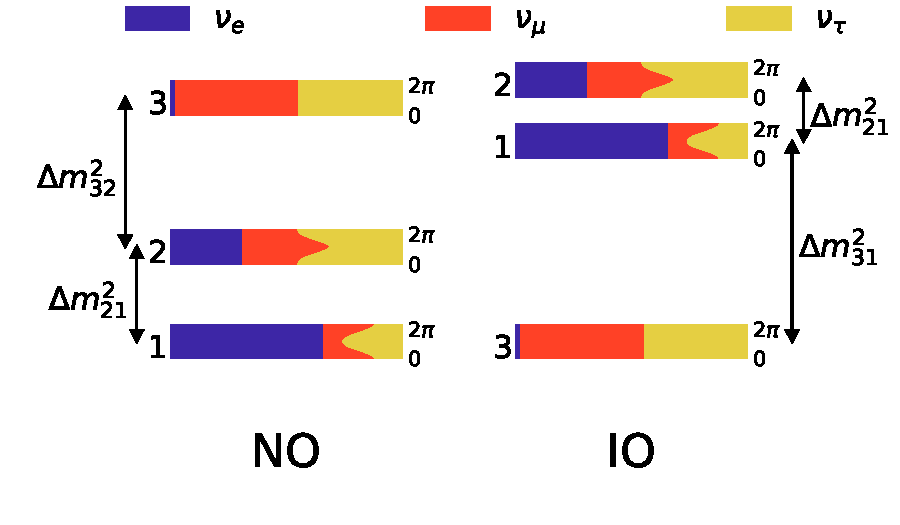
\includegraphics[width=\textwidth]{img/neutrinomassorderings.pdf}
\end{center}
\caption{Probability of finding a certain neutrino flavor in each neutrino mass eigenstate as the CP-violating phase, $\delta$, is
varied.  The left and right panels show the normal (NO) and inverted (IO) mass orderings, respectively. Neutrino masses increase from bottom to top. The electron, muon and tau flavor content of each neutrino mass eigenstate is shown via the blue, red and yellow fractions, respectively. Taken from \cite{DeSalas:2018rby}.}  \label{fig:numass_ordering}
\end{figure}
%%%%%

The absolute value of the neutrino mass scale can instead be probed via neutrinoless double beta decay searches, cosmological observations and beta decay experiments. Only upper bounds on the neutrino mass, of order $\sim$1 eV, currently exist. Constraints on the lightest neutrino mass coming from neutrinoless double beta decay will be discussed in sect.~\ref{subsec:bb0nu_lightmajoranaexchange}. In the following, we briefly summarize cosmological and beta decay constraints.

Primordial neutrinos have a profound impact on cosmology since they affect both the expansion history of the Universe and the growth of perturbations (see, for instance, reference \cite{Lesgourgues:2006nd}). Cosmological observations  can probe the sum of the three neutrino masses:
%
\begin{equation}
m_{{\rm cosmo}}\equiv \sum_{i=1}^3 m_i 
\label{eq:mcosmo}
\end{equation}
% 

Cosmological data are currently compatible with massless neutrinos. Several upper limit values on $m_{{\rm cosmo}}$ can be found in the literature, depending on the details of the cosmological datasets and of the cosmological model that were used in the analysis. A conservative upper limit of $m_{{\rm cosmo}} < 0.13$ eV at 95\% confidence level is obtained when Cosmic Microwave Background (CMB) temperature measurements from the Planck satellite \cite{Planck:2018vyg} are combined with the most recent Baryon Acoustic Oscillation (BAO) measurements from the Sloan Digital Sky Survey (SDSS) galaxy surveys including eBOSS \cite{eBOSS:2020yzd}, in the framework of a Lambda Cold Dark Matter ($\Lambda$CDM) model with dark energy whose equation of state is fixed to $-1$. Even the use of Planck CMB temperature and polarization data alone yields a very robust, and competitive, limit $m_{{\rm cosmo}} < 0.26$ eV at 95\% CL \cite{Planck:2018vyg}.
The relationship between $m_{{\rm cosmo}}$, defined in eq.~(\ref{eq:mcosmo}), and the lightest neutrino mass $m_{{\rm light}}$ ---that is, $m_1$ ($m_3$) in the case of normal (inverted) ordering--- is shown in the top panel of fig.~\ref{fig:mass_constraints_cosmo_beta}. The two bands correspond to the normal and inverted orderings, respectively. The width of the bands is given by the 3$\sigma$ ranges in the mass oscillation parameters $\Delta m^2_{{21}}$ and $\Delta m^2_{{31}}$ \cite{Esteban:2020cvm}. The horizontal band in the top panel of fig.~\ref{fig:mass_constraints_cosmo_beta} is the upper limit on $m_{{\rm cosmo}}$. The $m_{{\rm cosmo}} < 0.13$ eV upper bound translates into a limit of $m_{{\rm light}}\lesssim 0.034\ {\rm eV}$ at 95\% CL in the normal ordering case, as shown by the vertical dashed line in the top panel of fig.~\ref{fig:mass_constraints_cosmo_beta}, and into an even stricter $m_{{\rm light}}$ bound in the inverted ordering case.

%%%%%
\begin{figure}[t!b!]
\begin{center}
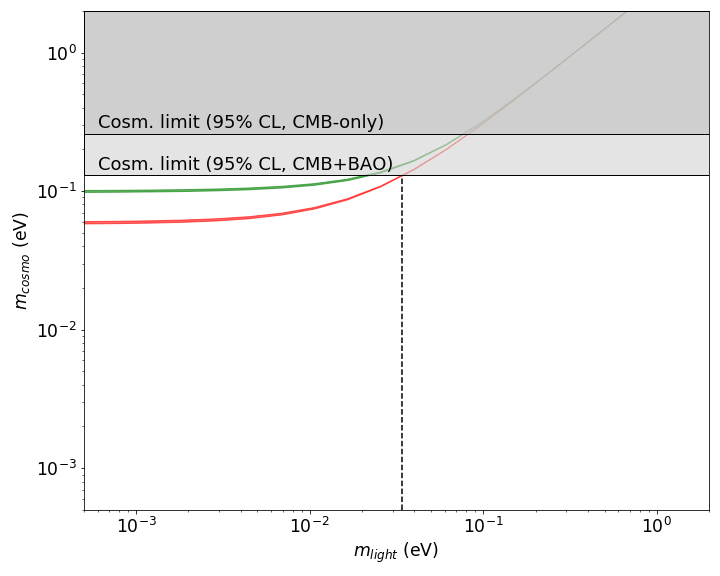
\includegraphics[width=0.7\textwidth]{img/mcosmovsmlight.png} 
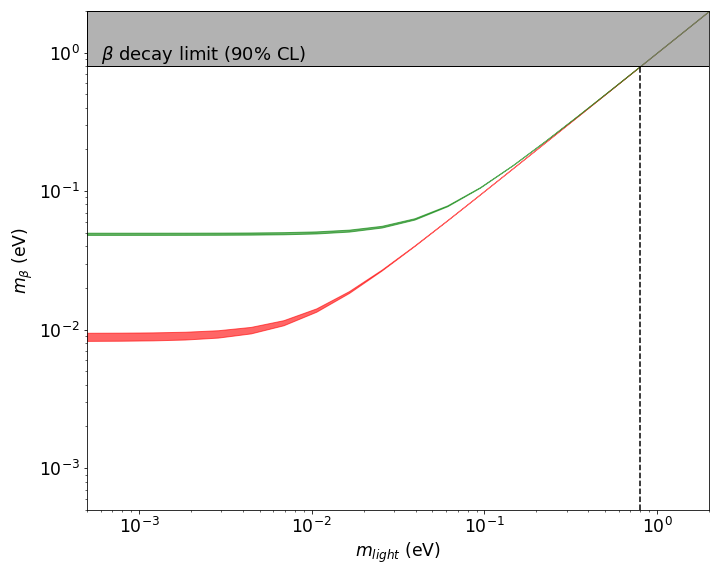
\includegraphics[width=0.7\textwidth]{img/mbetavsmlight.png}
\end{center}
\caption{\label{fig:mass_constraints_cosmo_beta}Constraints on the lightest neutrino mass $m_{\rm light}$ coming from cosmological (upper panel) and $\beta$ decay (lower panel) experiments. The red and green bands correspond to the normal and inverted orderings, respectively. The $m_{{\rm cosmo}}$ and $m_{\beta}$ upper bounds in the top and bottom panels are from \cite{eBOSS:2020yzd} and \cite{KATRIN:2021uub}, respectively. They translate into the $m_{{\rm light}}$ upper limits shown via the vertical dashed lines.}
\end{figure}
%%%%%

The neutrino mass scale can also be probed in laboratory-based experiments (see, for example, \cite{Otten:2008zz}). The differential electron energy spectrum in nuclear $\beta$ decay experiments is affected both by the neutrino masses and by the mixings defining the electron neutrino state in terms of mass eigenstates. In this case, the mass combination probed is given by:
%%%%%
\begin{equation}
m_{\beta}^2\equiv\sum_{i=1}^3\lvert U_{ei}\rvert^2m_i^2
\label{eq:mbeta}
\end{equation}
%%%%%

The relationship between $m_{\beta}$ in eq.~(\ref{eq:mbeta}) and $m_{{\rm light}}$ is shown in the bottom panel of fig.~\ref{fig:mass_constraints_cosmo_beta}. Again, the results of a recent global fit to neutrino oscillation data \cite{Esteban:2020cvm} are used to determine the $3\sigma$ bands for both the normal and inverted orderings. From the experimental point of view, the region of interest for the study of neutrino properties is located near the $\beta$ endpoint. The most sensitive searches conducted so far are based upon the decay of tritium, via $^3{\rm H}\to^3{\rm He}^+e^-\bar{\nu}_e$, mostly because of the very low $\beta$ endpoint energy of this element (18.6 keV). As for cosmology, $\beta$ decay searches of neutrino mass have so far yielded negative results. The horizontal band in the bottom panel of fig.~\ref{fig:mass_constraints_cosmo_beta} comes from the KATRIN experiment bound, $m_{\beta}<0.8$ eV at 90\% CL \cite{KATRIN:2021uub}. The resulting constraint on $m_{{\rm light}}$ is less stringent than the cosmological one, $m_{{\rm light}}\lesssim 0.8$ eV at 90\% CL. 

%%%%%%%%%%%%%%%%%%%%%%%%%%%%%%%%%%%%%%%%%%%%%%%%%%%%%%%%%%%%%%%%%%%%%%%%%%

\subsection{\label{subsec:massivenus_identity}The origin of neutrino mass: Dirac \emph{versus} Majorana neutrinos}

Are neutrinos their own antiparticles? If the answer is no, we speak of \emph{Dirac neutrinos}. If the answer is yes, we speak of \emph{Majorana neutrinos}. Both possibilities exist for the neutrino, being electrically neutral and not carrying any other charge-like conserved quantum number. Whether neutrinos are Majorana or Dirac particles depends on the nature of the physics that give them mass, given that the two characters are physically indistinguishable for massless neutrinos.

In the Standard Model, only the negative chirality component $\Psi_L$ of a fermion field $\Psi=\Psi_R+\Psi_L$ is involved in the weak interactions. A negative (positive) chirality field $\Psi_{L(R)}$ is a field that obeys the relations $P_{L(R)}\Psi_{L(R)}=\Psi_{L(R)}$ and $P_{R(L)}\Psi_{L(R)}=0$, where $P_L=(1-\gamma_5)/2$ and $P_R=(1+\gamma_5)/2$ are the positive and negative chiral projection operators. 

For massless neutrinos (see, for example, \cite{Hernandez:2010mi}), only the negative chirality neutrino field $\nu_L$ is needed in the theory, regardless of the Dirac/Majorana nature of the neutrino discussed below, since neutrinos only participate in the weak interactions. This field describes \emph{negative helicity} neutrino states $\lvert\nu_L\rangle$ and \emph{positive helicity} antineutrino states\footnote{As customarily done, we use the subscript ``L'' to denote both negative helicity states $\lvert\nu_L\rangle$ and negative chirality fields $\nu_L$, since the terms left-handed helicity states and left-handed chirality fields are also commonly used. Similarly, we denote positive helicity states and positive chirality fields with the subscript ``R'', as in ``right-handed''.}. The positive and negative helicity states are eigenstates of the helicity operator $h\equiv \vec{\sigma}\cdot\hat{p}$ with eigenvalues $\pm 1/2$, respectively, where $\vec{\sigma}$ is the neutrino spin and $\hat{p}$ the neutrino momentum direction. The fact that $\nu_L$ annihilates particles of negative helicity, and creates antiparticles with positive helicity, is not inconsistent with Lorentz invariance, given that the helicity is the same in any reference frame for a fermion travelling at the speed of light. In the Standard Model with massless neutrinos, positive helicity neutrinos and negative helicity antineutrinos do not exist. As a consequence, and since a negative helicity state transforms into a positive helicity state under the parity transformation, the chiral nature of the weak interaction (differentiating negative from positive chirality) implies that parity is maximally violated in the weak interactions.

For relativistic neutrinos of non-zero mass $m$, the neutrino field participating in the weak interactions has still negative chirality, $\nu_L$, but there are sub-leading corrections to the particle annihilation/creation rules described above. The state $\lvert\nu_L\rangle$ that is annihilated by the negative chirality field $\nu_{L}$ is now a linear superposition of the $-1/2$ and $+1/2$ helicity states. The $+1/2$ helicity state enters into the superposition with a coefficient $\propto m/E$, where $E$ is the neutrino energy, and is therefore highly suppressed. 

Neutrino mass terms can be added to the Standard Model Lagrangian in two ways (see, for example, \cite{Giunti:2003qt}). The first way is in direct analogy to the Dirac masses of quarks and charged leptons, by adding the positive chirality component $\nu_R$ of the Dirac neutrino field, describing predominantly positive helicity neutrino states and predominantly negative helicity antineutrino states that do not participate in the weak interactions:
%
\begin{equation}
\label{eq:diracmassterm}
-\mathcal{L}_D=m_D(\overline{\nu_L}\nu_R+\overline{\nu_R}\nu_L),
\end{equation}
%
where $m_D=y v/\sqrt{2}>0$, $y$ is a dimensionless Yukawa coupling coefficient and $v/\sqrt{2}$ is the vacuum expectation value of the neutral Higgs field after electroweak symmetry breaking. In eq.~(\ref{eq:diracmassterm}), $\nu_L$ and $\nu_R$ are, respectively, the negative and positive chirality components of the neutrino field $\nu$. The chiral spinors $\nu_L$ and $\nu_R$ have only two independent components each, leading to the four independent components in the spinor $\nu$. This is different from the case of massless neutrinos, where only the 2-component spinor $\nu_L$ was needed.

The second way in which neutrino mass terms can be added to the Standard Model Lagrangian is unique to neutrinos. Majorana first realized \cite{Majorana:1937vz} that, for neutral particles, one can remove two of the four degrees of freedom in a massive Dirac spinor by imposing the \emph{Majorana condition}:
%%%%%
\begin{equation}
\nu^c = \nu
\label{eq:majoranacondition}
\end{equation}
%%%%% 
where $\nu^c = C\bar{\nu}^T=C(\gamma^0)^T\nu^{\ast}$ is the CP conjugate of the field $\nu$, $C$ is the charge-conjugation operator, $(\nu_L)^c=(\nu^c)_R$ has positive chirality, and $(\nu_R)^c=(\nu^c)_L$ has negative chirality. This result can be obtained by decomposing both the left-hand and right-hand sides of eq.~(\ref{eq:majoranacondition}) into their chiral components, yielding:
%%%%%
\begin{equation}
\nu_R = (\nu_L)^c
\label{eq:nur}
\end{equation}
%%%%%
and therefore proving that the positive chirality component of the Majorana neutrino field $\nu_R$ is not independent of, but obtained from, its negative chirality counterpart $\nu_L$. By substituting eq.~(\ref{eq:nur}) into the mass term in eq.~(\ref{eq:diracmassterm}), we obtain a \emph{Majorana mass term}:
%%%%%
\begin{equation}
\label{eq:majoranamassterml}
-\mathcal{L}_L= \frac{1}{2}m_L(\overline{\nu_L}(\nu_L)^c+\overline{(\nu_L)^c}\nu_L)
\end{equation}
%%%%%
where $m_L$ is a free parameter with dimensions of mass. This Lagrangian mass term implies the existence of a weak isospin triplet scalar (a Higgs triplet), with a neutral component acquiring a non-vanishing vacuum expectation value after electroweak symmetry breaking. Equation (\ref{eq:majoranamassterml}) represents a mass term constructed from negative chirality neutrino fields alone, and we therefore call it a \emph{negative chirality Majorana mass term}. If positive chirality fields also exist and are independent of negative chirality ones, this is not the only possibility. In this case, we may also construct a second Majorana mass term, a \emph{positive chirality Majorana mass term}:
%%%%%
\begin{equation}
\label{eq:majoranamasstermr}
-\mathcal{L}_R= \frac{1}{2}m_R(\overline{\nu_R}(\nu_R)^c+\overline{(\nu_R)^c}\nu_R)
\end{equation}
%%%%%

In the Standard Model, right-handed fermion fields such as $\nu_R$ are weak isospin singlets. As a consequence, and in contrast with $m_D$ or $m_L$, the mass parameter $m_R$ is therefore not connected to a Higgs vacuum expectation value, and could be arbitrarily high. All three mass term in eqs.~(\ref{eq:diracmassterm}), (\ref{eq:majoranamassterml}) and (\ref{eq:majoranamasstermr}) convert negative chirality states into positive chirality ones\footnote{This is because the charge conjugate of a field with a given chirality, such as the ones appearing in eqs.~\ref{eq:majoranamassterml} and \ref{eq:majoranamasstermr}, always has the opposite chirality.}. Chirality is therefore not a conserved quantity, regardless of the Dirac/Majorana nature of neutrinos. Furthermore, the Majorana mass terms in eqs.~(\ref{eq:majoranamassterml}) and (\ref{eq:majoranamasstermr}) convert particles into their own antiparticles. As stated previously, they are therefore forbidden for all electrically charged fermions because of charge conservation. But not only: processes involving Majorana mass terms violate the Standard Model total lepton number $L\equiv L_e+L_{\mu}+L_{\tau}$ by two units ($\lvert\Delta L\rvert=2$), which is not a good quantum number anymore. 

Which of the mass terms allowed in theory, among $\mathcal{L}_D$, $\mathcal{L}_L$ and $\mathcal{L}_R$ in eqs.~(\ref{eq:diracmassterm}), (\ref{eq:majoranamassterml}) and (\ref{eq:majoranamasstermr}) exist in nature? What are the numerical values of the corresponding coupling constants $m_D$, $m_L$, $m_R$? These questions can in principle be answered experimentally. Majorana and Dirac massive neutrinos will in fact have different Standard Model interactions. Let us consider for now an instructive, albeit unrealistic, scattering experiment, see fig.~\ref{fig:DiracMajoranaNeutrinoInteractions}.

\begin{figure}[t!b!]
\begin{minipage}[t]{0.54\textwidth}
\vspace{0pt}
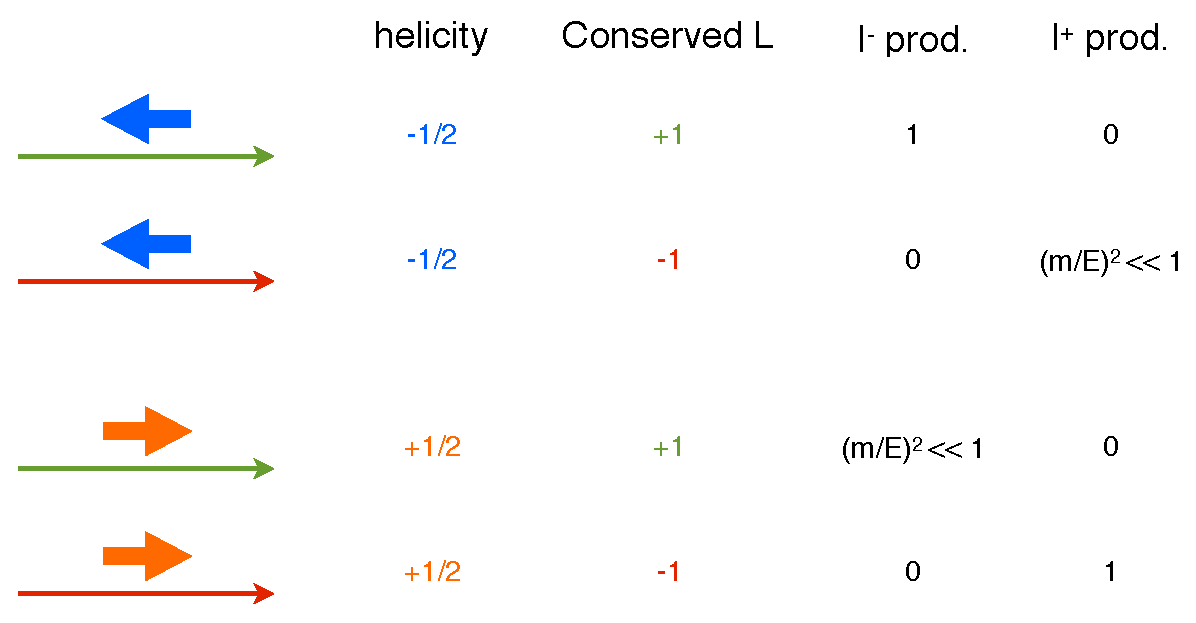
\includegraphics[width=\textwidth]{img/DiracNeutrinoInteraction.eps} % original figure size: 19.69 × 9.99 cm
\end{minipage}
\hfill
\begin{minipage}[t]{0.41\textwidth} % (14.93/19.69)*0.54=0.41
\vspace{0pt}
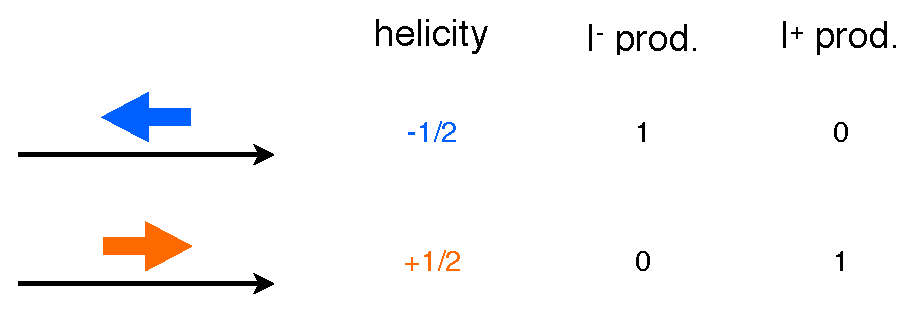
\includegraphics[width=\textwidth]{img/MajoranaNeutrinoInteraction.eps} % original figure size: 14.93 × 4.73 cm
\end{minipage} 
\caption{The difference between Dirac (left) and Majorana (right) massive neutrinos in a scattering experiment. See text for details. Adapted from \cite{Parke:2010sct}.}
\label{fig:DiracMajoranaNeutrinoInteractions}
\end{figure}

In the Dirac case, Standard Model interactions conserve lepton number $L$, with $L(\nu)=L(l^-)=-L(\bar{\nu})=-L(l^+)=+1$, where $l^{\pm}$ indicates charged leptons. Particles are then identified as neutrinos or antineutrinos in accordance with the process through which they are produced. Charged-current interactions of Dirac neutrinos (as opposed to antineutrinos) produce only $l^-$ and carry a well-defined lepton number $L=-1$, and vice versa. As shown in fig.~\ref{fig:DiracMajoranaNeutrinoInteractions}, for Dirac neutrinos we would thus have four mass-degenerate states: for each of the two available helicity states\footnote{As mentioned above, the weak interaction is maximally parity violating, therefore the two helicity states are distinguishable.}, two distinct particle/antiparticle states characterized by a different $L$ value would be available. Standard Model interactions of neutrino (as opposed to antineutrino) states of positive helicity would have, however, much weaker $l^-$-producing interactions with matter compared to neutrino states of negative helicity, as indicated by the coefficients in fig.~\ref{fig:DiracMajoranaNeutrinoInteractions}. On the other hand, we have seen that in the Majorana case $L$ is not conserved. We would only have two mass-degenerate states, defined by the two available helicity states, see fig.~\ref{fig:DiracMajoranaNeutrinoInteractions}.

Given these differences between Dirac and Majorana massive neutrinos, can we establish which of the two possibilities is realized in Nature via a scattering experiment? In practice, no. The reason is that $l^-$ production from positive helicity Dirac neutrinos (and $l^+$ production from negative helicity Dirac antineutrinos) is expected to be highly suppressed in the ultra-relativisitc limit, and cannot be experimentally observed. Experimentally, all we know is that the neutral particle produced in association with a $l^+$ produces, when interacting, a $l^-$. In the Dirac case, lepton number conservation is assumed, and such neutral particle is identified as the neutrino, with $L=-1$. In the Majorana case, such neutral particle is instead identified as the negative helicity state, interacting differently from its positive helicity counterpart. Both interpretations are viable, and what happens when a neutrino interacts can be understood without invoking a conserved lepton number \cite{Kayser:2002qs}.

Interestingly, the possible observation of the scattering of non-relativistic neutrinos has attracted recent attention. In the non-relativistic case, the difference between Majorana and Dirac neutrinos would become pronounced. The only source of non-relativistic neutrinos known in Nature is the Cosmic Neutrino Background (CNB). Strong indirect evidence for CNB neutrinos exists from cosmological probes, although the CNB has never been directly detected thus far. The neutrino capture on beta-decaying nuclei, such as tritium ($\nu$ + $^3$H $\to$ $^3$He + e$^-$) and first proposed by Weinberg \cite{Weinberg:1962zza}, is being explored by the PTOLEMY Collaboration for the CNB detection \cite{PTOLEMY:2019hkd}. The observation of such a process with sufficient event statistics would provide information on the Dirac/Majorana nature of neutrinos, considering that the capture rate for Majorana neutrinos can be up to a factor of two larger than the one for Dirac neutrinos \cite{Long:2014zva}.

%%%%%%%%%%%%%%%%%%%%%%%%%%%%%%%%%%%%%%%%%%%%%%%%%%%%%%%%%%%%%%%%%%%%%%%%%%

\subsection{\label{subsec:massivenus_seesaw}The see-saw mechanism}
%
\indent Neutrino masses, although not measured yet, are known to be small,
 of the order of 1 eV or less, see sect.~\ref{subsec:massivenus_whereweare}. Such mass values are much smaller than the masses of all other elementary fermions, see fig.~\ref{fig:particlemasses}. The explanation of neutrino masses via
 Dirac mass terms alone require neutrino Yukawa couplings of the
 order of $10^{-12}$ or less. The current theoretical prejudice is that
 neutrino Yukawa couplings with $y_{\nu}\ll 1$ and $y_{\nu}\ll y_l$
 are unnatural, if not unlikely. \\

%%%%%
\begin{figure}[t!b!]
\begin{center}
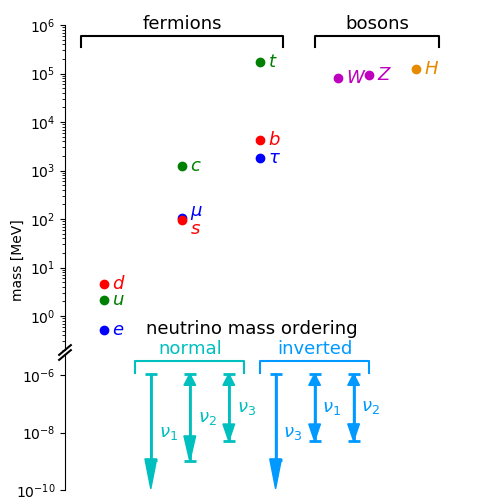
\includegraphics[width=0.75\textwidth]{img/masses.png}
\end{center}
\caption{ \label{fig:particlemasses}Hierarchical structure of elementary particle masses. Only upper bounds for neutrino masses exist. Both normal and inverted neutrino mass ordering scenarios are shown. Mass values are taken from \cite{ParticleDataGroup:2022pth}.}
\end{figure}
%%%%%

%
\indent The so-called \emph{see-saw mechanism} provides a way to accommodate
 neutrino masses that is considered more natural. The simplest realization of the see-saw model is to add both a Dirac mass term and a positive chirality mass term to the Lagrangian, as given by eqs. (\ref{eq:diracmassterm}) and (\ref{eq:majoranamasstermr}), respectively, for each of the three neutrino flavors. This is sometimes called the \emph{type I see-saw mechanism}, where we take $m_L=0$, $m_D\neq 0$, and $m_R\neq 0$. In this case, the neutrino mass terms can be recast in the matrix form:
%%%%%
\begin{equation}
-\mathcal{L}_{\text{D+R}}
=
\frac{1}{2} \,
\overline{(\mathcal{N}_L)^c} \, M \, \mathcal{N}_L
+
\text{h.c.}
\,,
\label{eq:seesawmatrixform}
\end{equation}
%%%%%
\noindent where the matrix $M$ has the form:
%%%%%
\begin{equation}
M
=
\begin{pmatrix}
0 & m_{\text{D}}
\\
m_{\text{D}} & m_R
\end{pmatrix}
\end{equation}
%%%%%
\noindent and the negative chirality vector $\mathcal{N}_L$ is
%%%%%
\begin{equation}
\mathcal{N}_L
=
\begin{pmatrix}
\nu_L
\\
(\nu_R)^c
\end{pmatrix}
\,.
\label{eq:typeIseesaw_1family}
\end{equation}
%%%%%

The chiral fields $\nu_L$ and $\nu_R$ do not have a definite mass, since they are coupled by the Dirac mass term. In order to find the fields $\nu_{1L}$ and $N_{1L}$ with definite masses $m_1$ and $M_1$, respectively, it is necessary to diagonalize the mass matrix in eq.~(\ref{eq:seesawmatrixform}). In other words, it is necessary to find a unitary mixing matrix $\mathcal{U}$ such that:
%%%%%
\begin{equation}
\mathcal{U}^T \, M \, \mathcal{U} =
\begin{pmatrix}
m_1 & 0
\\
0 & M_1
\end{pmatrix}
\,,
\label{eq:diagonalization_1family}
\end{equation}
%%%%%
\noindent where:
%%%%%
\begin{equation}
\mathcal{N}_L = \mathcal{U}  \, n_L
\,,
\qquad
\text{with}
\qquad
n_L
=
\begin{pmatrix}
\nu_{1L}
\\
N_{1L}
\end{pmatrix}
\,,
\label{eq:diagonalization2_1family}
\end{equation}
%%%%%

 For each neutrino flavor, two fields of definite chirality and definite mass are therefore obtained, and the diagonalized mass terms can be written as:
%%%%%
\begin{equation}
-\mathcal{L}_{D+R}
=
\frac{1}{2}
\left(m_1 \, \overline{(\nu_{1L})^c} \, \nu_{1L} + M_1 \, \overline{(N_{1L})^c} \, N_{1L}\right) + \text{h.c.}
\,,
\label{eq:diagonalization3_1family}
\end{equation}
%%%%%

Both terms in eq.~(\ref{eq:diagonalization3_1family}) have the same form as the pure negative chirality Majorana mass term in eq.~(\ref{eq:majoranamassterml}). In other words, both mass eigenfields $\nu_{1L}$ and $N_{1L}$ are equal to their CP-conjugate fields, and thus both describe Majorana particles. The insertion of a Dirac mass term and a positive chirality Majorana mass term in the Lagrangian for massive neutrinos has resulted in Majorana particles.

Since the positive chirality fields are electroweak singlets in the Standard Model, the Majorana mass of the neutrino described by such field, $m_R$, may be orders of magnitude larger than the electroweak scale. In the so-called \emph{see-saw limit}, we assume that neutrino Yukawa couplings are of the order of the charged fermion couplings, and that $m_R\gg m_D$ is of the order of some high mass scale where new physics responsible for neutrino masses is supposed to reside. In this approximation, the see-saw mechanism naturally yields a small mass eigenvalue $m_1\simeq m_D^2/m_R\ll m_D$ for a predominantly negative helicity neutrino mass state, and a large mass eigenvalue $M_1\simeq m_R$ for a predominantly positive helicity (and therefore sterile) neutrino mass state. A very heavy $N_1$ corresponds to a very light $\nu_1$ and vice versa, as in a see-saw. 

The see-saw mechanism presented above can easily be generalized from the one-family case that we discussed to three neutrino species, yielding the three light neutrinos $\nu_i$ we are familiar with, and three heavy neutrinos $N_i$, with $i=1,2,3$ \cite{Giunti:2003qt}. In this case, the neutrino mass matrix in eq.~\ref{eq:seesawmatrixform} is a $6\times6$ mass matrix of the form:
%
\begin{equation}
M
=
\begin{pmatrix}
0 & (M^{\text{D}})^T
\\ \displaystyle
M^{\text{D}} & M^R
\end{pmatrix}
\,.
\label{eq:diagonalization_3families}
\end{equation}
%
\noindent where $M^D$ and $M^R$ are now $3\times3$ complex matrices, and the 6-component vector of negative chirality fields has the form:
%
\begin{equation}
N_L
=
\begin{pmatrix}
\nu_L
\\ \displaystyle
(\nu_R)^c
\end{pmatrix}
\,,
\qquad
\text{with}
\qquad
\nu_L
=
\begin{pmatrix}
\nu_{eL}
\\ \displaystyle
\nu_{{\mu}L}
\\ \displaystyle
\nu_{{\tau}L}
\end{pmatrix}
\qquad
\text{and}
\qquad
(\nu_R)^c
=
\begin{pmatrix}
(\nu_{s_1 R})^c
\\ \displaystyle
(\nu_{s_2 R})^c
\\ \displaystyle
(\nu_{s_3 R})^c
\end{pmatrix}
\,,
\label{eq:diagonalization_3families_2}
\end{equation}
%
In eq.~\ref{eq:diagonalization_3families_2}, the subscripts $e,\ \mu,\ \tau$ label the active neutrino flavors, while the subscripts $s_1,\ s_2,\ s_3$ indicate sterile states that do not participate in the weak interactions. The mass matrix is diagonalized via a $6\times6$ mixing matrix $\mathcal{V}$ analogous to $\mathcal{U}$ in eq.~\ref{eq:diagonalization_1family}, where the three negative chirality fields and the three positive chirality fields are now expressed in terms of the negative chirality components of 6 massive neutrino fields $\nu_{iL},\ i=1,\ldots ,6$. In the see-saw limit where the eigenvalues of $M^R$ are much larger than those of $M^D$, the $6\times6$ mass matrix in eq.~\ref{eq:diagonalization_3families} can be written in block-diagonal form $M\simeq \text{diag}(M_{\text{light}},M_{\text{heavy}})$, where the two $3\times3$ mass matrices of the light and heavy neutrino sectors are practically decoupled, and given by $M_{\text{light}}\simeq -(M^D)^T(M^R)^{-1}M^D$ and $M_{\text{heavy}}\simeq M^R$, respectively. 

For the low-energy phenomenology, it is sufficient to consider only $M_{\text{light}}$, sometimes called the \emph{neutrino mass matrix} $m_{\nu}$, that is the $3\times3$ matrix in the flavor basis which is diagonalized by the matrix $U$:
%
\begin{equation}
U^T \, M_{\text{light}} \, U
=
\text{diag}\!\left(m_1,m_2,m_3\right)
\,,
\label{eq:diagonalization3_3families}
\end{equation}
%
\noindent where the \emph{neutrino mixing matrix} $U$ appearing in eq.~(\ref{eq:diagonalization3_3families}) is the same matrix defined in eq.~(\ref{eq:neutrinomixing}), and $m_1,\ m_2,\ m_3$ are three light neutrino mass eigenvalues discussed in sect.~\ref{subsec:massivenus_whereweare}.

An important assumption in the simplest realization of the see-saw mechanism described above is that $m_L=0$. This assumption is not arbitrary, and directly follows from enforcing the gauge symmetries of the Standard Model, see for example \cite{Giunti:2003qt}. 

There exist other realizations of the see-saw mechanism, which differ from the Type-I mechanism in the nature of the new heavy degrees of freedom that are added to the Standard Model. While three gauge-singlet fermions are introduced in Type-I, Type-II and Type-III) see-saw models add one gauge-triplet scalar and three gauge-triplet fermions, respectively. 

%%%%%%%%%%%%%%%%%%%%%%%%%%%%%%%%%%%%%%%%%%%%%%%%%%%%%%%%%%%%%%%%%%%%%%%%%%


\subsection{\label{subsec:massivenus_leptogenesis}Leptogenesis}

Inflationary models of the Universe predict matter and antimatter to be equally abundant at the very hot beginning, given that any potential initial asymmetry would have been diluted away by inflation. However, the observable Universe today is almost entirely made of matter! This matter dominance today is consistent with the small level of baryon asymmetry that is inferred from BBN and CMB observations, given that annihilation of matter with antimatter would have left us in a matter-dominated Universe today. The baryon asymmetry has been precisely measured \cite{ParticleDataGroup:2022pth,Planck:2018vyg}:
%
\begin{equation}
\eta \equiv \frac{n_B-n_{\bar{B}}}{n_{\gamma}} = 274\times 10^{-10}\Omega_bh^2 = (6.12\pm 0.04)\times 10^{-10} \label{eq:measuredbaryonasymmetry}
\end{equation}
%
where $n_B$, $n_{\bar{B}}$, $n_{\gamma}$ are the number densities of baryons, antibaryons and photons, $\Omega_bh^2=(0.0224\pm 0.0001)$ is the fraction of the critical energy density carried by baryons, and $h\equiv H_0/100\ \text{km}\cdot\text{s}^{-1}\cdot\text{Mpc}^{-1}=(0.674\pm 0.005)$ is the Hubble parameter, where $H_0$ is the Hubble constant today.

%%%%%
\begin{figure}[t!b!]
\begin{center}
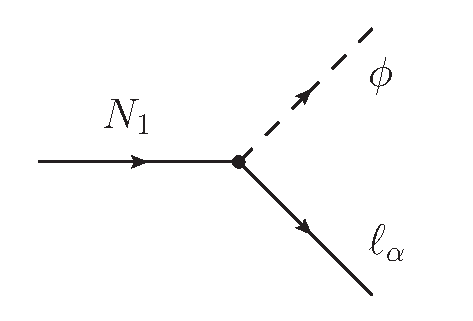
\includegraphics[width=0.32\textwidth]{img/leptog1.eps} \hfill
\raisebox{0.2cm}{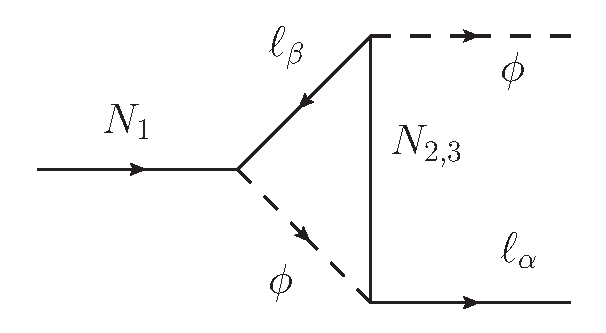
\includegraphics[width=0.32\textwidth]{img/leptog2.eps}} \hfill
\raisebox{0.2cm}{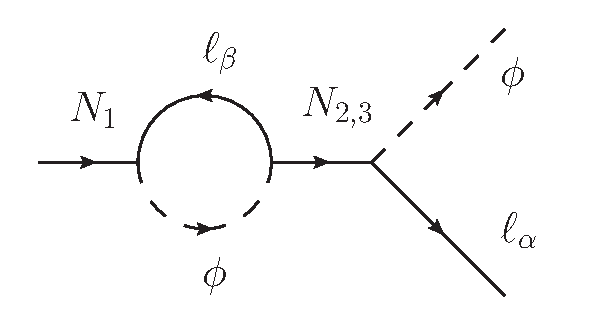
\includegraphics[width=0.32\textwidth]{img/leptog3.eps}}
\end{center}
\caption{Feynman diagrams that contribute to the lepton number asymmetry through the decays of the heavy Majorana neutrino $N_1$ into the Higgs $\phi$ plus leptons $l_{\alpha}$. The asymmetry is generated via the interference of the tree-level diagram (left) with the one-loop vertex correction (center) and the self-energy (right) diagrams (adapted from \cite{Chen:2007fv}).} \label{fig:leptogenesis}
\end{figure}
%%%%%

What caused this matter-antimatter asymmetry in the early Universe? The baryon asymmetry could have been induced by a lepton asymmetry: \emph{leptogenesis} (see, for example, \cite{Chen:2007fv,Davidson:2008bu}). If neutrinos are Majorana particles, the decays of the heavy Majorana neutrinos into leptons $l_{\alpha}$ plus Higgs particles $\phi$ in the early Universe provides an ideal scenario for leptogenesis. Heavy Majorana neutrinos are their own anti-particles, so they can decay to both $l_{\alpha}\phi$ and $\bar{l_{\alpha}}\bar{\phi}$ final states. If there is an asymmetry in the two decay rates, a net lepton asymmetry will be produced. Figure \ref{fig:leptogenesis} shows the processes that would contribute to a net lepton asymmetry in the presence of heavy Majorana neutrino decays, in the simplest case where the asymmetry is dominated by the decay of the lightest among the three heavy neutrinos, $N_1$. Finally, this lepton asymmetry can be efficiently converted into a baryon asymmetry via the so-called \emph{sphaleron processes} (see \cite{Chen:2007fv,Davidson:2008bu} for details).

In more detail, for leptogenesis to occur, three conditions must be met. These conditions directly follow from the ingredients that are required to dynamically generate a baryon asymmetry (\emph{Sakharov's conditions} \cite{Sakharov:1967dj}): 
\begin{enumerate}
\item Presence of lepton number violating processes;
\item Beyond-SM sources of CP violation\footnote{CP violation is allowed by the Standard Model and has been measured; however, the magnitude of such CP-violating effects is far too small to provide the necessary amount of leptogenesis.};
\item Departure from thermal equilibrium, so that the inverse processes do not wash out the generated lepton asymmetry.
\end{enumerate}
 The decay of heavy Majorana neutrinos can provide all of these conditions, namely
\begin{enumerate}
\item Total lepton number is violated in these decays;
\item CP can be violated in these decays, provided that there is more than one heavy Majorana field;
\item Departure from thermal equilibrium is obtained if the decay rate is slower than the expansion rate of the Universe at the time of decoupling, occurring for $T\sim M_1$, where $T$ is the temperature of the Universe's thermal bath, and $M_1$ is the mass of the lightest among the three heavy neutrinos. 
\end{enumerate}
%%%%%
In order to be fully successful, any theory of leptogenesis must be able to explain the observed magnitude of baryon asymmetry given in eq.~(\ref{eq:measuredbaryonasymmetry}). Leptogenesis via heavy Majorana neutrino decays is in principle able to do this. In this case, the asymmetry in lepton flavor $\alpha$ produced in the decay of $N_1$, defined as:
%%%%%
\begin{equation}
\varepsilon_{\alpha\alpha}\equiv \frac{\Gamma(N_1\to \phi l_{\alpha})-\Gamma(N_1\to\bar{\phi} \bar{l}_{\alpha})}{\Gamma(N_1\to \phi l)+\Gamma(N_1\to\bar{\phi} \bar{l})}
\label{eq:letptogenesis_asymmetry}
\end{equation}
%%%%%
\noindent should be of order $\lvert\varepsilon_{\alpha\alpha}\rvert>10^{-7}$ \cite{Davidson:2008bu}, where the factors $\Gamma$ in eq.~(\ref{eq:letptogenesis_asymmetry}) stand for the decay rates into the corresponding $N_1$ decay final states. It is at present unclear whether there is a direct connection between the high-energy CP-violating processes responsible for the asymmetry in the early Universe of eq.~(\ref{eq:letptogenesis_asymmetry}), and the low-energy CP-violating processes that may potentially affect laboratory-based experiments. Nonetheless, the discovery of CP violation in the lepton sector via neutrino oscillations on the one hand, and the discovery of the Majorana nature of neutrinos via neutrinoless double beta decay on the other, would undoubtedly strengthen the case for leptogenesis as a source of the baryon asymmetry of the Universe.

%%%%%%%%%%%%%%%%%%%%%%%%%%%%%%%%%%%%%%%%%%%%%%%%%%%%%%%%%%%%%%%%%%%%%%%%%%


\subsection{\label{subsec:massivenus_lviolation}Lepton number violating processes}

We have seen that Majorana mass terms induce lepton number violating processes of the type $\lvert\Delta L\rvert=2$. The Majorana nature of the heavy neutrino needed for leptogenesis, discussed in sect.~\ref{subsec:massivenus_leptogenesis}, implies lepton number violating processes. However, this decay is unobservable in a laboratory-based experiment, given the tremendous energies needed for the production of such a heavy neutrino\footnote{For strongly hierarchical heavy neutrino masses, a lower bound on the right-handed neutrino mass from leptogenesis of order $10^9$~GeV is obtained \cite{Davidson:2002qv}.}. A number of more promising lepton number violating processes have been proposed to probe the Majorana nature of neutrinos. The best known example is \bbonu, the subject of this review and introduced in sect.~\ref{sec:bb0nu}. We anticipate that \bbonu\ is considered the most promising probe of the Majorana nature of neutrinos. However, and because of neutrino mixing, the phenomenology associated with $\lvert\Delta L\rvert=2$ processes is very rich. The basic process with $\lvert\Delta L\rvert=2$ is mediated by \cite{Atre:2005eb}:
%%%%%
\begin{equation}
W^-W^-\to l^-_{\alpha}l^-_{\beta}
\label{eq:dl2process}
\end{equation}
%%%%%
\noindent and we can categorize such processes according to the lepton flavors $(\alpha,\beta)$ involved. Assuming no lepton flavor violating contributions other than light Majorana neutrino exchange, the matrix element for the generic $\lvert\Delta L\rvert=2$ process in eq.~(\ref{eq:dl2process}) is proportional to the element $(\alpha,\beta)$ of the \emph{neutrino mass matrix}:
%%%%%
\begin{equation}
\left(m_{\nu}\right)_{\alpha\beta}\equiv \left(U^{\ast}\text{diag}(m_1,m_2,m_3)U^{\dagger}\right)_{\alpha\beta}=
 \sum_{i=1}^3 U^{\ast}_{\alpha i}U^{\ast}_{\beta i}m_i
\label{eq:mnu}
\end{equation}
%%%%%
\noindent where $m_{\nu}=M^{\text{light}}$ is the matrix appearing in eq.~(\ref{eq:diagonalization3_3families}), $U_{\alpha i}$ are the elements of the 3$\times$3 neutrino mixing matrix appearing in eq.~\ref{eq:neutrinomixing}, and $m_i$ are the three light neutrino masses. In a sense, this effective neutrino mass definition provides a metric to compare the sensitivity of various $\lvert\Delta L\rvert=2$ processes. The processes with the most competitive constraints on $\lvert\Delta L\rvert=2$ processes involving the flavors $(\alpha,\beta)$ are reported in table \ref{tab:lviol_processes}. \\

%%%%%
\begin{table}[t!b!]
\caption{\label{tab:lviol_processes}Current bounds on effective neutrino masses from total lepton number violating processes, organized according to the flavors involved. Numbers taken (or derived) from \cite{ParticleDataGroup:2022pth,Atre:2005eb}.}
%\begin{tabular}{llll} \hline
\begin{tabular}{p{0.10\textwidth}p{0.16\textwidth}p{0.40\textwidth}p{0.20\textwidth}}
\toprule
Flavors & Method & Experimental bound & Mass bound (eV) \\ \midrule
%
$(e,e)$ & \bbonu & $T_{1/2}(\Xe{136} \to \Ba{136}+2e^-)>1.07 \times 10^{26}\ \mathrm{yr}$ & $\lvert m_{ee}\rvert < 6.1\times 10^{-2}$ \\ \midrule
%
$(e,\mu)$ & $\mu^- \to e^+$ & $\Gamma(\mathrm{Ti}+\mu^- \to e^+ +\mathrm{Ca}_{\rm gs})\ /\ \Gamma(\text{Ti}+\mu^-\text{capture})<1.7 \times 10^{-12}$ & $\lvert m_{e\mu}\rvert < 1.7 \times 10^7$ \\ \midrule
%
$(e,\tau)$ & $\tau$ decays & $\Gamma(\tau^-\to e^+\pi^-\pi^-)\ /\ \Gamma_{\text{tot}}<2.0 \times 10^{-8}$ & $\lvert m_{e\tau}\rvert < 1.2 \times 10^{12}$ \\ \midrule
%
$(\mu,\mu)$ & K decays & $\Gamma(K^+\to \pi^-\mu^+\mu^+)\ /\ \Gamma_{\text{tot}}<4.2 \times 10^{-11}$ & $\lvert m_{\mu\mu}\rvert < 5.7 \times 10^{7}$ \\ \midrule
%
$(\mu,\tau)$ & $\tau$ decays & $\Gamma(\tau^-\to \mu^+\pi^-\pi^-)\ /\ \Gamma_{\text{tot}}<3.9 \times 10^{-8}$ & $\lvert m_{e\tau}\rvert < 2.2 \times 10^{12}$ \\ \midrule
%
$(\tau,\tau)$ & none & none & none \\ \bottomrule
\end{tabular}
\end{table}
%%%%%

As is apparent in table \ref{tab:lviol_processes}, indeed, the constraint on the effective Majorana mass $m_{ee}$ coming from \bbonu\ searches outperforms by several orders of magnitude other searches involving a different flavor combination $(\alpha,\beta)$. The most important reason behind this is of statistical nature. While it is possible to amass macroscopic quantities of a \bb\ emitter to study \bbonu\ decay (as we will see, even $\mathcal{O}$(1 ton) of isotope is in the cards of several experiments), this is not the case for the other experimental techniques listed in table \ref{tab:lviol_processes}. Nevertheless, it is important to keep exploring lepton flavor violating processes other than \bbonu\ for two reasons. First, it is in principle possible that phase cancellations are such that $m_{ee} \ll m_{\alpha\beta}$ with $(\alpha,\beta)\neq (e,e)$, making the search for \bbonu\ much less favorable than others because of Nature's choice of neutrino masses and mixings. Second, this effort may lead to the identification of an even most promising experimental probe of lepton flavor violation in the future.



\section{Neutrinoless double beta decay} \label{sec:bb0nu}
\subsection{Double beta decay modes} \label{subsec:bbmodes}
%
Double beta decay is a rare nuclear transition in which a nucleus with $Z$ protons decays into a nucleus with $Z+2$ protons and the same mass number $A$. The decay can occur only if the initial nucleus is less bound than the final nucleus, and both more than the intermediate one, as shown in Fig.~\ref{fig:atomicmasses_a136}. Such a condition is fulfilled by 35 nuclides in nature because of the nuclear pairing force (see Sect.~\ref{subsec:manybody}), ensuring that nuclei with even $Z$ and $N$ are more bound than the odd-odd nuclei with the same $A=Z+N$.

\begin{figure}[tb]
\centering
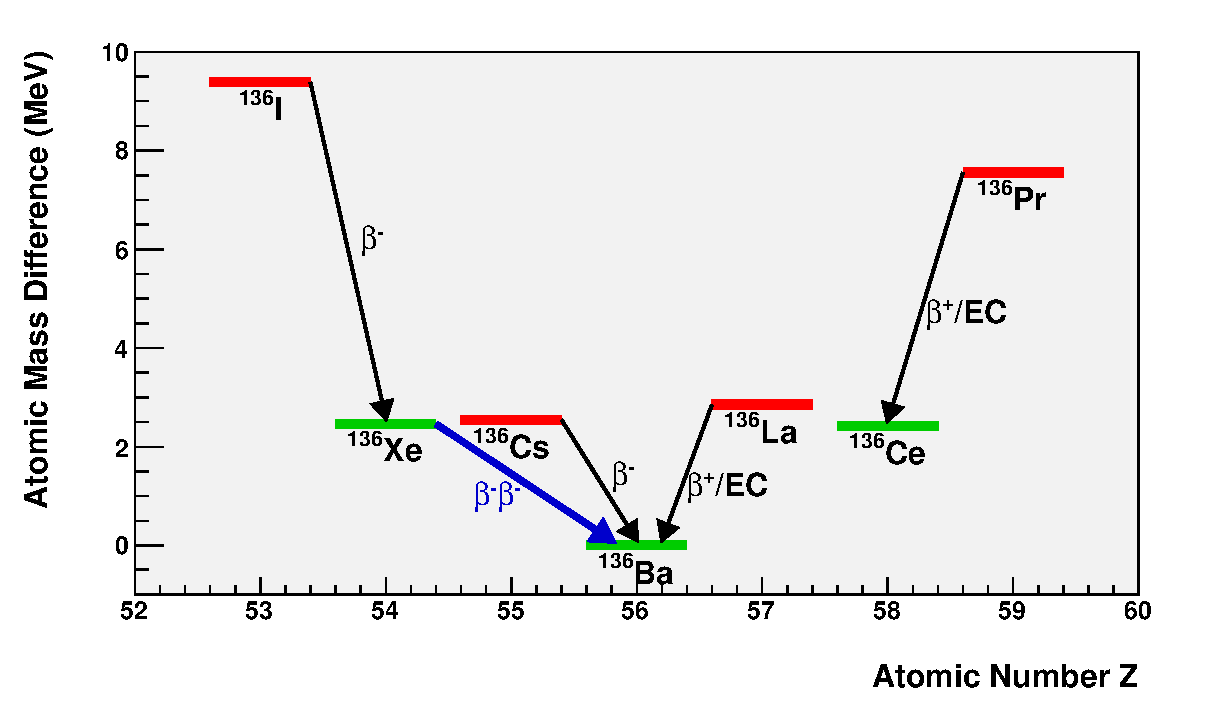
\includegraphics[width=\textwidth]{img/atomicmasses_a136.eps}
\caption{Atomic masses of isotopes with $A=136$ given as differences with respect to the most bound isotope, \Ba{136}. The red (green) levels indicate odd-odd (even-even) nuclei. The arrows $\beta^-$, $\beta^+$, $\beta^-\beta^-$ indicate nuclear decays accompanied by electron, positron and double electron emission, respectively. The arrows EC indicate electron capture transitions.} \label{fig:atomicmasses_a136}
\end{figure}

The standard decay mode (\bbtnu), consisting of two simultaneous beta decays,
\begin{equation}
(Z,A) \rightarrow (Z+2,A) + 2\ e^{-} + 2\ \overline{\nu}_{e},
\label{eq:bb2nu}
\end{equation}
was first considered by Maria Goeppert-Mayer in 1935 \cite{Goeppert-Mayer:1935uil}. Total lepton number is conserved in this mode, and the process is allowed in the Standard Model of particle physics. This process was first detected in 1950 using geochemical techniques \cite{Inghram:1950qv}. The first direct observation of \bbtnu\ events, in \Se{82} and using a time projection chamber, did not happen until 1987 \cite{Elliott:1987kp,Moe:2014ioa}. Since then, it has been repeatedly observed in several nuclides. Typical lifetimes are of the order of $10^{19}$--$10^{21}$ years, among the longest ever observed among radioactive decay processes\footnote{To our knowledge, only the closely related two-neutrino double electron capture process of \Xe{124}, with a half-life of $(1.8\times 0.5)\times 10^{22}$~yr \cite{XENON:2019dti}, has been measured directly to have a longer half-life than the \bbtnu\ processes in Table~\ref{tab:bb2nu_exp}.}. For a list of \bbtnu\ half-lives measured in several isotopes, see Table~\ref{tab:bb2nu_exp} \cite{Barabash:2020nck}. The longest half-life in Table~\ref{tab:bb2nu_exp} is the one for \Xe{136}, which was measured for the first time only in 2011 \cite{EXO-200:2011xzf}.

%%%%%
\begin{table}[tb]
\caption{Current best direct measurements of the half-life of \bbtnu\ processes.  The values reported are taken from the averaging procedure described in \cite{Barabash:2020nck}.} \label{tab:bb2nu_exp}
\begin{center}
%\begin{tabular}{rcc}
\begin{tabular}{p{0.10\textwidth}p{0.22\textwidth}p{0.55\textwidth}}
\toprule
Isotope & $T_{1/2}^{2\nu}\ \text{(year)}$ & Experiments \\ \midrule
%
\Ca{48} & $(5.3^{+1.2}_{-0.8}) \times 10^{19}$ & Irvine TPC \cite{Balysh:1996vr}, TGV \cite{Brudanin:2000in}, NEMO-3 \cite{NEMO-3:2016mvr}  \\
%
\Ge{76} & $(1.88\pm 0.08)\times 10^{21}$ & HEIDELBERG-MOSCOW \cite{Dorr:2003gf}, GERDA \cite{Agostini:2015nwa}  \\
%
\Se{82} & $(0.87\pm ^{+0.02}_{-0.01})\times 10^{20}$ & NEMO-3 \cite{Arnold:2018tmo}, CUPID-0 \cite{Azzolini:2019yib}, Irvine TPC \cite{Elliott:1992cf}, NEMO-2 \cite{NEMO:1997rel}   \\
%
\Zr{96} & $(2.3\pm 0.2)\times 10^{19}$ & NEMO-2 \cite{Arnold:1999vg}, NEMO-3 \cite{NEMO-3:2009fxe} \\
%
\Mo{100} & $(7.06^{+0.15}_{-0.13})\times 10^{18}$ & NEMO-3 \cite{NEMO-3:2019gwo}, CUPID-Mo \cite{Armengaud:2019rll}, NEMO-2 \cite{NEMO:1994sst}, Irvine TPC \cite{DeSilva:1997cp}, ZnMoO$_4$ bolometers \cite{Cardani:2013mja}  \\
%
\Cd{116} & $(2.69\pm 0.09)\times 10^{19}$ & NEMO-3 \cite{NEMO-3:2016zfx}, Aurora \cite{Barabash:2018yjq}, ELEGANT \cite{Ejiri:1995kd}, Solotvina \cite{Danevich:2003ef}, NEMO-2 \cite{NEMO:1996gxj}   \\
%
\Te{130} & $(7.91\pm 0.21)\times 10^{20}$ & CUORE-0 \cite{CUORE:2016ons}, CUORE \cite{Nutini:2020vtd}, CUORICINO \cite{Arnaboldi:2002te}, NEMO-3 \cite{NEMO-3:2011wyg}  \\
%
\Xe{136} & $(2.18\pm 0.05)\times 10^{21}$ & EXO-200 \cite{EXO-200:2013xfn}, KamLAND-Zen \cite{KamLAND-Zen:2016pfg} \\
%
\Nd{150} & $(9.34\pm 0.65)\times 10^{18}$ & NEMO-3 \cite{NEMO-3:2016qxo}  \\
\botrule
\end{tabular}
\end{center}
\end{table}
%%%%%

The neutrinoless mode (\bbonu),
\begin{equation}
(Z,A) \rightarrow (Z+2,A) + 2\ e^{-},
\label{eq:bb0nu}
\end{equation}
was first proposed by W.~H.~Furry in 1939 \cite{Furry:1939qr} as a method to test Majorana's theory \cite{Majorana:1937vz} applied to neutrinos. In contrast to the two-neutrino mode, the neutrinoless mode violates total lepton number conservation and is therefore forbidden in the Standard Model. Its existence is linked to that of Majorana neutrinos (see Sect.~\ref{subsec:bb0nu_blackbox}). No convincing experimental evidence of the decay exists to date. 
%(see Sect.~\ref{subsec:bb0nu_expstatus}).

The two modes of the \bb\ decay have some common and some distinct features \cite{Vogel:2008sx}. The common ones are:
\begin{itemize}
    \item The leptons carry essentially all the available energy, and the nuclear recoil is negligible.
    \item The transition involves the $0^+$ ground state of the initial nucleus and, in almost all cases, the $0^+$ ground state of the final nucleus. For some isotopes, it is energetically possible to have a transition to an excited $0^+$ or to a $2^+$ final state,\footnote{The transition to an excited $0^+$ final state has been observed for both $^{100}\text{Mo}$ \cite{Barabash:1995fn,Barabash:1999dp,Kidd:2009ai,NEMO:2006smm,Belli:2010zzc,NEMO-3:2014pkc} and $^{150}\text{Nd}$ \cite{Barabash:2009wy,Kidd:2014hra,Polischuk:2021bwl}.} even though they are suppressed because of the smaller phase space available.
    \item Both processes are second-order weak processes, \emph{i.e.} their rate is proportional to $G_F^4$, where $G_F$ is the Fermi constant. They are therefore inherently slow. Phase space considerations alone would give preference to the \bbonu\ mode, which is, however, forbidden by total lepton number conservation. 
\end{itemize}

The distinct features are:
\begin{itemize}
    \item In the \bbtnu\ mode, the sum electron kinetic energy $T_1+T_2$ spectrum is continuous and peaked below $Q_{\beta\beta}/2$, where $Q_{\beta\beta}$ is the Q-value of the reaction. In the \bbonu\ mode, since no light particles other than the electrons are emitted and given that nuclear recoil is negligible, the $T_1+T_2$ spectrum is a mono-energetic line at $Q_{\beta\beta}$, smeared only by the detector resolution. This is illustrated in Fig.~\ref{fig:modes}.
    \item The \bbtnu\ mode probes momentum transfers of order $\mathcal{O}(Q_{\beta\beta})\simeq \mathcal{O}$(1~MeV), while the \bbonu\ reaction probes much higher momentum transfers of order $\mathcal{O}(m_{\pi})\simeq \mathcal{O}$(100~MeV).
\end{itemize}

In addition to the two basic decay modes described above, several decay modes involving the emission of a light neutral boson, the Majoron ($\chi^{0}$), have been proposed in extensions of the Standard Model, see Sect.~\ref{subsec:bb0nu_alternativemechanisms}.


\begin{figure}[t]
\vspace{1cm}
\begin{center}
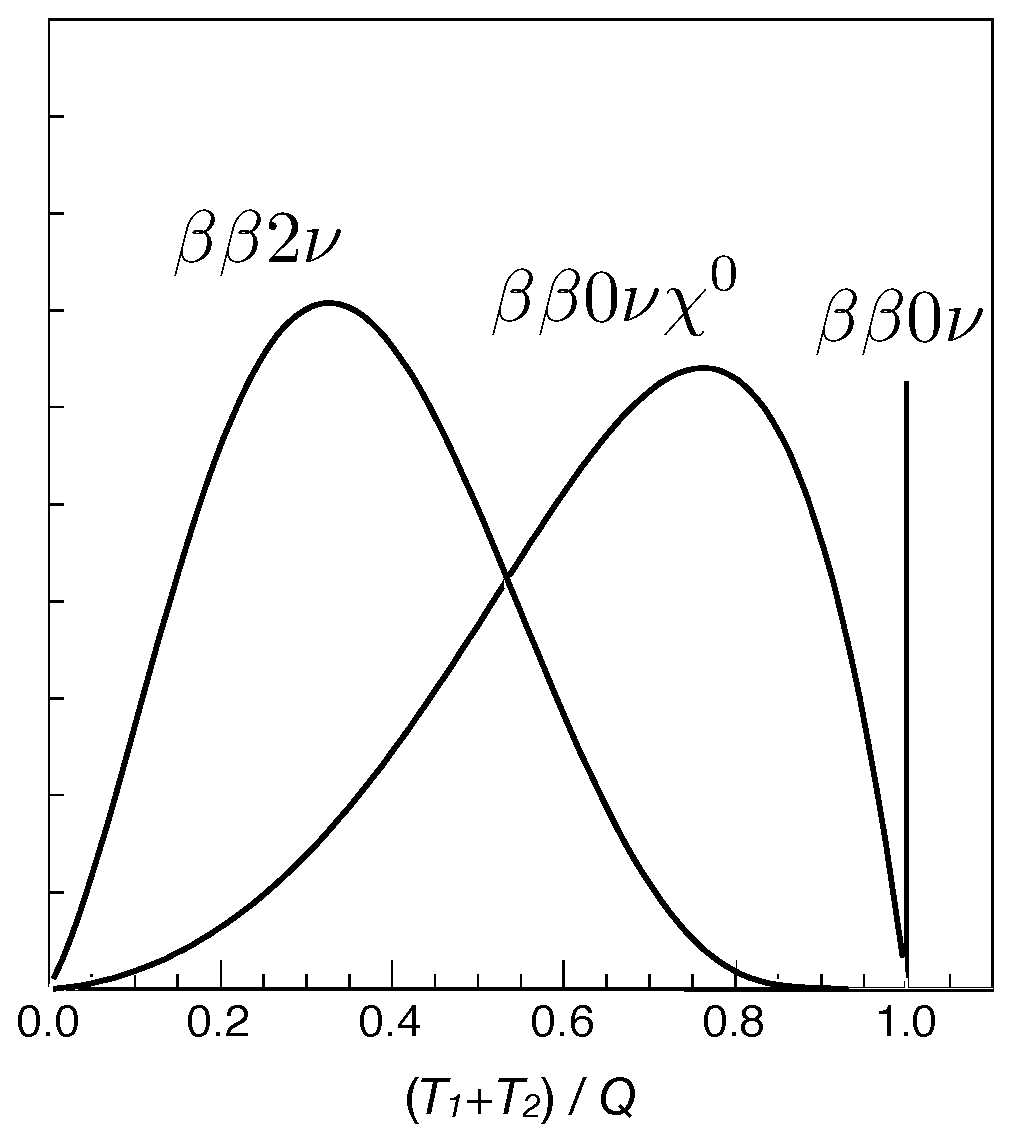
\includegraphics[angle=0,scale=0.325]{img/modes.eps}
\end{center}
\caption{Spectra for the sum kinetic energy $T_1+T_2$ of the two electrons, for different \bb\ modes: \bbtnu, \bbonu, and \bb\ decay with Majoron emission.} \label{fig:modes}
\end{figure}

While in the following we will focus on \bbonu\ as defined in Eq.~(\ref{eq:bb0nu}), there are three closely related lepton number violating processes that can be investigated:
%
\begin{eqnarray}
\beta^+\beta^+0\nu: & (Z,A) \to (Z-2,A) + 2\ e^+  \label{eq:b+b+}\\
\beta^+\text{EC}0\nu: & e^- + (Z,A) \to (Z-2,A) + e^+ \label{eq:b+EC}\\
\text{ECEC}0\nu: & 2\ e^- + (Z,A) \to (Z-2,A)^\ast \label{eq:ECEC}
\end{eqnarray}
%
Such processes are called \emph{double positron emission}, \emph{single positron emission plus single electron capture} (EC), and \emph{double electron capture}, respectively. All three involve transitions where the nuclear charge decreases (as opposed to increasing, as in \bbonu) by two units. From the theoretical point of view, the physics probed by $\beta^+\beta^+0\nu$, $\beta^+\text{EC}0\nu$ and $\text{ECEC}0\nu$ is identical to the one probed by \bbonu. From the experimental point of view, however, $\beta^+\beta^+0\nu$ and $\beta^+\text{EC}0\nu$ are less favorable than \bbonu\ because of the smaller phase space available. On the other hand, the process $\text{ECEC}0\nu$ is gaining some attention recently as a promising (but still much less developed) alternative to \bbonu, since a resonant enhancement of its rate can in principle occur \cite{Eliseev:2011zza}.

In the following, the neutrinoless mode \bbonu\ is discussed in more detail, from both the theoretical and experimental point of views.

\subsection{The black box theorem } \label{subsec:bb0nu_blackbox}
In general, in theories beyond the Standard Model there may be several sources of total lepton number violation which can lead to \bbonu. Nevertheless, as it was first pointed out in reference \cite{Schechter:1981bd}, irrespective of the mechanism, \bbonu\ necessarily implies Majorana neutrinos. This is called the \emph{black box} (or Schechter-Valle) theorem. The reason is that any $\Delta L\neq 0$ diagram contributing to the decay would also contribute to the $(e,e)$ entry of the Majorana neutrino mass matrix, $(m_{\nu})_{ee}$. This is shown in fig.~\ref{fig:blackbox}, where a $\bar{\nu}_e-\nu_e$ transition, that is a non-zero $(m_{\nu})_{ee}$, is induced as a consequence of any $\Delta L\neq 0$ operator responsible for \bbonu.

From a quantitative point of view, however, the diagram in fig.~\ref{fig:blackbox} corresponds to a tiny (of order $\mathcal{O}(10^{-28}~\mathrm{eV})$) mass generated at the four-loop level, and is far too small to explain the neutrino mass splittings observed in neutrino oscillation experiments \cite{Duerr:2011zd}. Other, unknown, Majorana and/or Dirac mass contributions must exist. As a consequence, therefore, the black box theorem says nothing about the physics mechanism dominating a \bbonu\ rate that is large enough to be observable. The dominant mechanism leading to \bbonu\ could then either be directly connected to neutrino oscillations phenomenology, or only indirectly connected or not connected at all to it \cite{Rodejohann:2011mu}. The former case is realized in the standard \bbonu\ mechanism of light neutrino exchange, discussed in Sect.~\ref{subsec:bb0nu_lightmajoranaexchange}. The latter case involves alternative \bbonu\ mechanisms, briefly outlined in Sect.~\ref{subsec:bb0nu_alternativemechanisms}.

\begin{figure}[t!b!]
\begin{center}
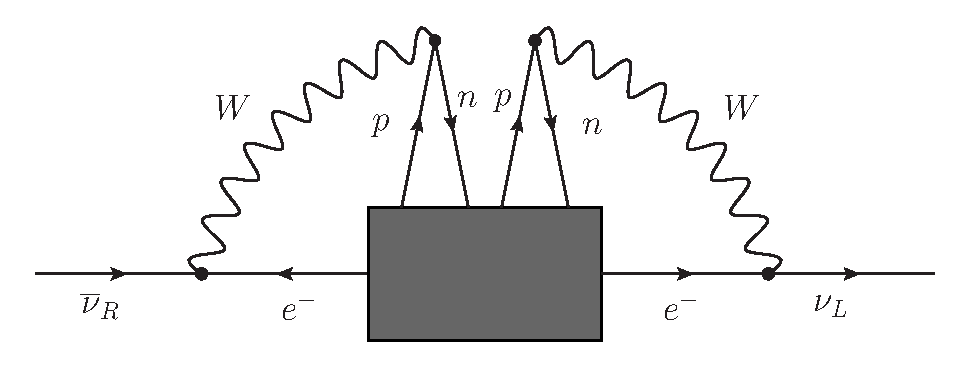
\includegraphics[scale=0.65]{img/blackbox.eps}
\end{center}
\caption{Diagram showing how any neutrinoless double beta decay process induces a $\bar{\nu}$-to-$\nu$ transition, that is, an effective Majorana mass term. This is the so-called \emph{black box theorem} \cite{Schechter:1981bd}.} \label{fig:blackbox}
\end{figure}


\subsection{The standard neutrinoless double beta decay mechanism: light Majorana neutrino exchange} \label{subsec:bb0nu_lightmajoranaexchange}

Neutrinoless double beta decay can arise from a diagram (fig.~\ref{fig:bb0nu_standardmechanism}) in which the parent nucleus emits a pair of virtual $W$ bosons, and then these $W$ exchange a Majorana neutrino to produce the outgoing electrons. The rate is non-zero only for massive, Majorana neutrinos. The reason is that the exchanged neutrino in fig.~\ref{fig:bb0nu_standardmechanism} can be seen as emitted (in association with an electron) with almost total positive helicity. Only its small, $\mathcal{O}(m/E)$, negative helicity component is absorbed in the other vertex by the Standard Model electroweak current. Considering that the amplitude is in this case a sum over the contributions of the three light neutrino mass states $\nu_i$, and that is also proportional to $U_{ei}^2$, we conclude that the modulus of the amplitude for the \bbonu\ process must be proportional in this case to the \emph{effective neutrino Majorana mass}:
%
\begin{equation}
\mbb \equiv \lvert \sum_{i=1}^{3} m_i U_{ei}^2 \rvert. \label{eq:mbb}
\end{equation}
%
In other words, the effective neutrino Majorana mass corresponds to the modulus of the $(e,e)$ element of the neutrino mass matrix of eq.~(\ref{eq:mnu}), $\mbb\equiv \lvert (m_{\nu})_{ee}\rvert$.

%%%%%
\begin{figure}[t!b!]
\begin{center}
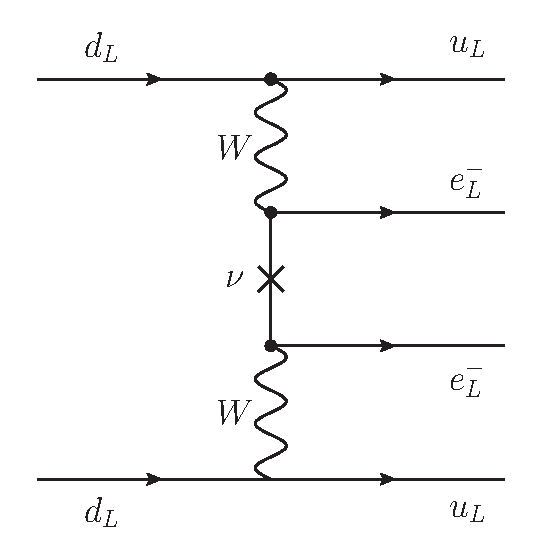
\includegraphics[scale=0.55]{img/FD_lightnu.eps}
\end{center}
\caption{\label{fig:bb0nu_standardmechanism}The standard mechanism for \bbonu\ decay, based on light Majorana neutrino exchange.}   
\end{figure}
%%%%%

In the case where light Majorana neutrino exchange is the dominant contribution to \bbonu, the inverse of the half-life for the process can be written as \cite{Doi:1985dx}:
%
\begin{equation}
\frac{1}{T^{0\nu}_{1/2}} = G^{0\nu}(Q,Z)\ \lvert M^{0\nu}\rvert^2\ \mbb^2,
\label{eq:Tonu}
\end{equation}
%
where \Gonu\ is a phase space factor that depends on the transition $Q$-value and on the nuclear charge $Z$, and $M^{0\nu}$ is the nuclear matrix element (NME). The phase space factor can be calculated analytically, in principle, with reasonable accuracy\footnote{An accurate description of the effect of the nuclear Coulomb field on the decay electron wave-functions is, however, required.}. The  NME is evaluated using nuclear models, although with considerable uncertainty (see Sect.~\ref{sec:nme}).
In other words, the value of the effective neutrino Majorana mass \mbb\ in eq.~(\ref{eq:mbb}) can be inferred from a non-zero \bbonu\ rate measurement, albeit with some nuclear physics uncertainties. Conversely, if a given experiment does not observe the \bbonu\ process, the result can be interpreted in terms of an upper bound on \mbb.  

If light Majorana neutrino exchange is the dominant mechanism for \bbonu, it is clear from eq.~(\ref{eq:mbb}) that \bbonu\ is in this case directly connected to neutrino oscillations phenomenology, and that it also provides direct information on the absolute neutrino mass scale, as cosmology and $\beta$ decay experiments do (see Sect.~\ref{subsec:massivenus_whereweare}). The relationship between \mbb\ and the actual neutrino masses $m_i$ is affected by:
%
\begin{enumerate}
\item the uncertainties in the measured oscillation parameters;
\item the unknown neutrino mass ordering (normal or inverted);
\item the unknown phases in the neutrino mixing matrix (both Dirac and Majorana). 
\end{enumerate}
%

For example, the relationship between \mbb\ and the lightest neutrino mass $m_{\text{light}}$ (which is equal to $m_1$ or $m_3$ in the normal and inverted mass ordering cases, respectively) is illustrated in fig.~\ref{fig:mbetabetavsmlight}. This graphical representation was first proposed in \cite{Vissani:1999tu}. The width of the two bands is due to items 1 and 3 above, where the uncertainties in the measured oscillation parameters (item 1) are taken as $3\sigma$ ranges from a recent global oscillation fit \cite{Esteban:2020cvm}. Figure \ref{fig:mbetabetavsmlight} also shows a 90\% confidence level upper bound on \mbb\ from current \bbonu\ data ($m_{\beta\beta}<0.036-0.156\ \text{eV}$). As can be seen from fig.~\ref{fig:mbetabetavsmlight}, current \bbonu\ data provide a constraint on the absolute mass scale $m_{\text{light}}$ that is more competitive than the current one from $\beta$ decay experiments, although less competitive as the cosmological one.
%
\begin{figure}[t!b!]
\begin{center}
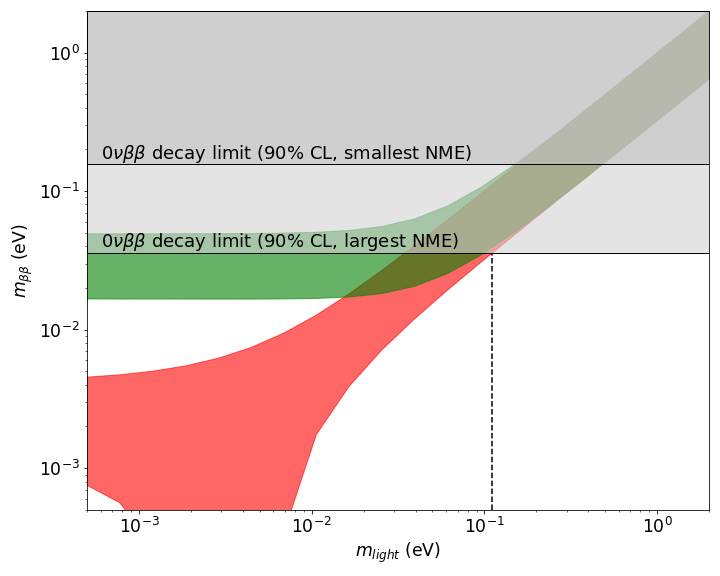
\includegraphics[width=0.7\textwidth]{img/mbetabetavsmlight.png}
\end{center}
\caption{\label{fig:mbetabetavsmlight}The effective neutrino Majorana mass \mbb\ as a function of the lightest neutrino mass, $m_{\text{light}}$. The red (green) band corresponds to the normal (inverted) ordering, respectively, in which case $m_{\text{light}}$ is equal to $m_1$ ($m_3$). The horizontally-excluded region comes from \bbonu\ constraints.}
\end{figure}

In figs.~\ref{fig:mass_constraints_cosmo_beta} and \ref{fig:mbetabetavsmlight}, we have shown only upper bounds on various neutrino mass combinations, coming from current data. The detection of positive results for absolute neutrino mass scale observables would open up the possibility to further explore neutrino properties and lepton number violating processes. We give three examples in the following. First, the successful determination of both $m_{\beta}$ in eq.~(\ref{eq:mbeta}) and \mbb\ in eq.~(\ref{eq:mbb}) via $\beta$ and \bbonu\ decay experiments, respectively, can in principle be used to determine or constrain the phases $\alpha_{i}$ \cite{Avignone:2007fu}. Second, measurements of $m_{\beta}$ or $m_{\text{cosmo}}$ in eq.~(\ref{eq:mcosmo}) may yield a constraint on $m_{\text{light}}$ that is inconsistent with a \mbb\ upper limit. In this case, the non-observation of \bbonu\ would suggest that neutrinos are Dirac particles. Third, measurements of $m_{\beta}$ or $m_{\text{cosmo}}$ may yield a constraint on $m_{\text{light}}$ that is inconsistent with a measured non-zero \mbb. This scenario would demonstrate that additional lepton number violating physics, other than light Majorana neutrino exchange, is at play in the \bbonu\ process. We briefly describe some of these possible \bbonu\ alternative mechanisms in the following.


\subsection{Alternative neutrinoless double beta decay mechanisms} \label{subsec:bb0nu_alternativemechanisms}
A number of alternative \bbonu\ mechanisms have been proposed. For an excellent and complete discussion of those, we refer the reader to \cite{Rodejohann:2011mu}. The realization of \bbonu\ can differ from the standard mechanism in one or several aspects:
%
\begin{itemize}
\item The Lorentz structure of the currents. Positive chirality currents mediated by a $W_R$ boson can arise, for example, in left-right symmetric theories. A possible diagram involving positive chirality current interactions of heavy Majorana neutrinos $N_i$ is shown in fig.~\ref{fig:nonstandardmechanisms}(a).
%
\item The mass scale of the exchanged virtual particles. One example would be the presence of ``sterile'' (that is, described by positive chirality fields) neutrinos, either light or heavy, in the neutrino propagator of fig.~\ref{fig:bb0nu_standardmechanism}, in addition to the three light, active, neutrinos we are familiar with. Another example would be the exchange of heavy supersymmetric particles, as in fig.~\ref{fig:nonstandardmechanisms}(b).
%
\item The number of particles in the final state. A popular example involves decay modes where additional Majorons, that are very light or massless particles which can couple to neutrinos, are produced in association with the two electrons (see fig.~\ref{fig:nonstandardmechanisms}(c)).
\end{itemize}
%
\begin{figure}[t!b!]
\begin{center}
\begin{tabular}{ccc}
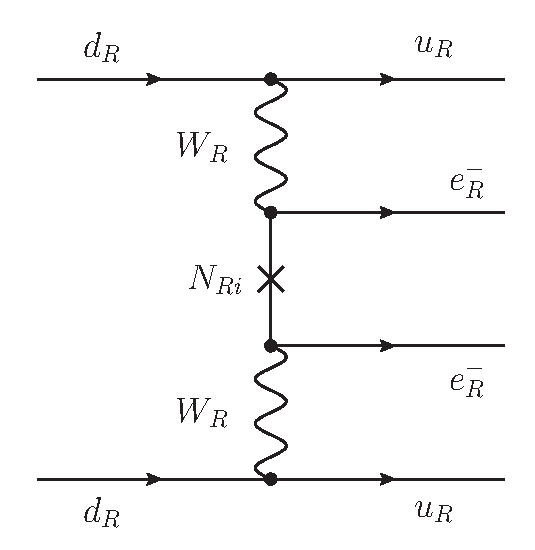
\includegraphics[width=0.30\textwidth]{img/FD_heavyNR_LR.eps} &
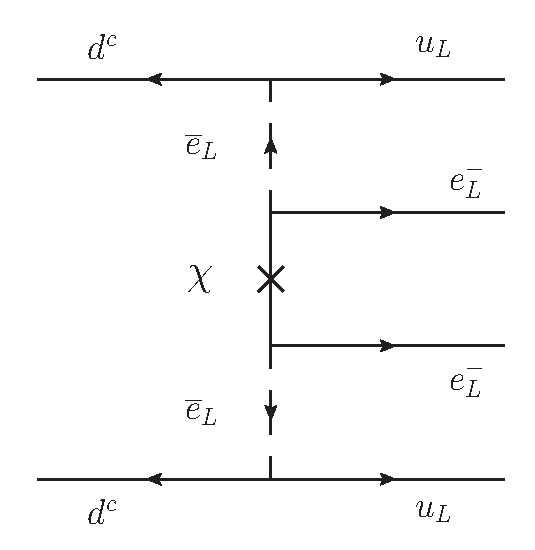
\includegraphics[width=0.30\textwidth]{img/FD_RPV_1a.eps} &
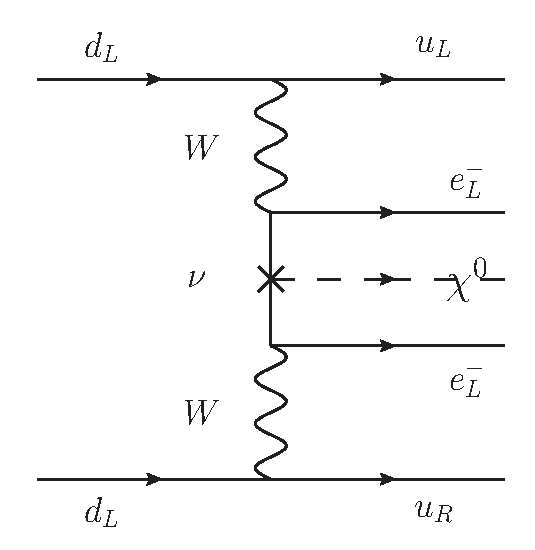
\includegraphics[width=0.30\textwidth]{img/FD_Majoron.eps} \\
(a) & (b) & (c) \\
\end{tabular}
\end{center}
\caption{\label{fig:nonstandardmechanisms}Examples of non-standard mechanism for \bbonu: (a) heavy neutrino exchange with positive chirality currents \cite{Mohapatra:1986pj}; (b) neutralino exchange in R-parity violating supersymmetry \cite{Mohapatra:1986su}; (c) Majoron emission \cite{Georgi:1981pg}.}   
\end{figure}
%
In non-standard \bbonu\ mechanisms, the scale of the lepton number violating physics is often larger than the characteristic nuclear Fermi momentum scale $\mathcal{O}$(100~MeV), in which case one speaks of \emph{short-range} processes. This is the case when the \bbonu\ process is mediated by heavy particles. It is in contrast to the standard \bbonu\ mechanism of light Majorana neutrino exchange, in which case the neutrino is very light compared to this momentum transfer scale, resulting in a \emph{long-range} process. Non-standard and long-range \bbonu\ processes are, however, also possible.

In general, several contributions to the total \bbonu\ amplitude can add coherently, allowing for interference effects. Neutrinoless double beta decay observables alone may be able to identify the dominant mechanism responsible for \bbonu. We give three examples. First, if Majorons are also emitted in association with the two electrons, energy conservation alone requires the electron kinetic energy sum $T_1+T_2$ to be a continuous spectrum with $Q_{\beta\beta}$ as endpoint. This spectrum is potentially distinguishable from the \bbtnu\ one (see fig.~\ref{fig:modes}), provided that the Majoron-neutrino coupling constant is large enough. Second, if positive chirality current contributions dominate the \bbonu\ rate, electrons will be emitted predominantly as positive helicity states. As a consequence, both the energy and angular correlation of the two emitted electrons will be different from the ones of the standard \bbonu\ mechanism. A detector capable of reconstructing individual electron tracks may therefore be able to distinguish this type of non-standard \bbonu\ mechanism from light Majorana neutrino exchange (see, for example, \cite{SuperNEMO:2010wnd}). Third, the combined observation of \bbonu\ decays to both ground and excited states of the daughter isotope may also shed light on the \bbonu\ mechanism. Neutrinoless double beta decays to excited states are however harder to search for, given the lower reaction Q-values and hence lower predicted rates. On the other hand, their experimental signature would be very characteristic, with typically one or two gamma rays emitted in coincidence with the two decay electrons. 
%

%\subsection{Existing experimental results} \label{subsec:bb0nu_expstatus}
%Neutrinoless double beta decay searches have been carried out over more than half a century, exploiting the same experimental techniques used for measuring the two-neutrino mode rate. Several \bb\ emitting isotopes have been investigated, as shown in table \ref{tab:bb0nu_exp}. Table~\ref{tab:bb0nu_exp} shows the best current \bbonu\ limits for the same 9 isotopes for which direct \bbtnu\ decay direct measurements exist, and includes also a recent limit for \Te{128}  (for which a direct measurement of the two-neutrino mode remains elusive).
%
%\begin{table}[t!b!]
%\centering
%\caption{\label{tab:bb0nu_exp}Current best limits on the half-life of \bbonu\ processes for the most interesting isotopes. All values are at 90\% CL.}
%\begin{tabular}{rcl}
%\toprule
%Isotope & $T_{1/2}^{0\nu}\ \text{(years)}$ & Experiment \\ \midrule
%%
%\Ca{48} & $>5.8 \times 10^{22}$ & ELEGANT VI \cite{Umehara:2008ru} \\
%%
%\Ge{76} & $>1.8 \times 10^{26}$ & GERDA \cite{GERDA:2020xhi} \\
%%
%\Se{82} & $>4.6 \times 10^{24}$ & CUPID-0 \cite{CUPID:2022puj} \\
%%
%\Zr{96} & $>9.2 \times 10^{21}$ & NEMO-3 \cite{NEMO-3:2009fxe}  \\
%%
%\Mo{100} & $>1.8 \times 10^{24}$ & CUPID-Mo \cite{Augier:2022znx}  \\
%%
%\Cd{116} & $>2.2 \times 10^{23}$ & Aurora \cite{Barabash:2018yjq}   \\
%%
%\Te{128} & $>3.6 \times 10^{24}$ & CUORE \cite{CUORE:2022piu} \\
%%
%\Te{130} & $>2.2 \times 10^{25}$ & CUORE \cite{CUORE:2021mvw} \\
%%
%\Xe{136} & $>2.3 \times 10^{26}$ & KamLAND-Zen \cite{KamLAND-Zen:2022tow} \\
%%
%\Nd{150} & $>2.0 \times 10^{22}$ & NEMO-3 \cite{NEMO-3:2016qxo} \\
%\bottomrule
%%\end{narrowtabular}
%\end{tabular}
%\end{table}
%%%%%%
%
%The most sensitive half-life limit to date was set by the xenon-based KamLAND-Zen experiment \cite{KamLAND-Zen:2022tow}: $\Tonu(\Xe{136}) > 2.3 \times 10^{26}$ years (90\% CL), corresponding to an effective Majorana mass bound of $\mbb < 0.036-0.151$~eV, where the range covers  commonly adopted nuclear matrix element calculations. Particularly competitive limits also exist for \Ge{76} and \Te{130}. For \Ge{76}, the GERDA experiment reported final half-life and Majorana mass limits of $\Tonu(\Ge{76})>1.8\times 10^{26}$~yr and $\mbb<0.079-0.180$~eV at 90\% CL, respectively \cite{GERDA:2020xhi}. For \Te{130}, the latest limits from the CUORE experiment are $\Tonu(\Te{130})>2.2\times 10^{25}$~yr and $\mbb<0.090-0.305$~eV at 90\% CL, respectively \cite{CUORE:2021mvw}. It is worth noting that, despite its lower half-life reach, the CUORE result is almost as competitive as the KamLAND-Zen and GERDA ones in terms of Majorana mass reach. As we will see in Sections \ref{sec:nme} and \ref{sec:ingredients}, this is due to the favorable phase space factor and nuclear matrix element of \Te{130}, compared to \Xe{136} and \Ge{76}.   
%








\section{Calculating nuclear matrix elements} \label{sec:nme}

The $0\nu\beta\beta$ decay half-life has been introduced in Eq.~\eqref{eq:Tonu} for a decay mediated by the exchange of light neutrinos. We recover the standard definition of the NME by factoring out the hadron coupling, $g_A$~\cite{Engel:2016xgb,Agostini:2022zub},
\begin{align}
T_{1/2}^{-1} =  G^{0\nu}\left(Q,Z\right)\,g_A^4\,\left(M^{0\nu}_\text{light}\right)^2\,m^2_{\beta\beta}\,,
\label{eq:master}
\end{align}
where $M^{0\nu}_\text{light}$ emphasizes that this NME only corresponds to the many-body part and to light-neutrino exchange\footnote{In eq.~\ref{eq:master}, the term $G^{0\nu}$ is expressed in yr$^{-1}\cdot$eV$^{-1}$ units. Alternatively, this equation is often written dividing $m^2_{\beta\beta}$ by the electron mass squared. In the latter case, $G^{0\nu}$ would have yr$^{-1}$ units.}.
As discussed in Sec.~\ref{sec:bb0nu}, the half-life necessarily depends on an unknown parameter that describes the mechanism beyond the standard model of particle physics responsible for the violation of lepton number in the decay, this is, for the creation of matter without antimatter. In the light-neutrino exchange scenario this parameter is $m_{\beta\beta}$, as illustrated in Eqs.~\eqref{eq:Tonu} and~\eqref{eq:master}. Therefore, as discussed in Sec.~\ref{subsec:bb0nu_lightmajoranaexchange}, in order to gain information on new physics after the $0\nu\beta\beta$-decay discovery, the remaining components of the half-life must be reliably known. Moreover, a good knowledge of these parts allows one to estimate the reach, in terms of the parameter space explored, of experimental proposals targeting a given half-life sensitivity~\cite{Agostini:2021kba}.

The components of the $0\nu\beta\beta$-decay rate within the standard model of particle physics in Eq.~\eqref{eq:master} cover the atomic physics related to the emitted electrons ---through the phase-space factor of the transition, $G^{0\nu}\left(Q,Z\right)$--- and the structure of the initial and final nuclear states ---through the NME, $M^{0\nu}_\text{light}$. In addition, $g_A$ represents the hadron coupling of the interaction to nucleons (protons or neutrons), which are the degrees of freedom used by many-body methods used to calculate the NMEs.
% , while the fundamental interaction driving the decay happens at the level of quarks and gluons ---the degrees of freedom of the underlying theory, quantum chromodynamics (QCD)---, 
Nonetheless, Eq.~\eqref{eq:master} is a simplification in the sense that various components contribute to $M^{0\nu}_\text{light}$, and they appear associated with different couplings at the nucleon level, not only $g_A$. These aspects are explained in detail in Sec.~\ref{subsec:nme_parts}.

\begin{figure}[t]
	\begin{center}
	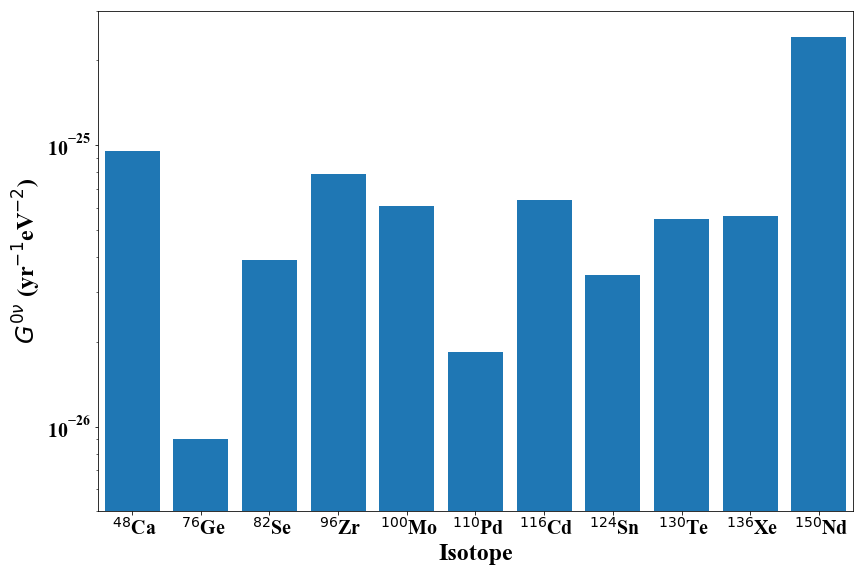
\includegraphics[width=0.8\textwidth]{img/g0nu.png} 	\caption{Phase-space factors $G^{0\nu}$ appearing in eq.~\ref{eq:master}, for all 11 \bb emitters with \Qbb$>2$~MeV. Values taken from \cite{Kotila:2012zza}.
 \label{fig:phase_space}}
	\end{center}
\end{figure}

Phase-space factors are quite accurately known for all relevant nuclei used in $0\nu\beta\beta$ decay experiments~\cite{Kotila:2012zza,Stoica:2013lka}. Figure~\ref{fig:phase_space} shows the corresponding values for the light-neutrino exchange mechanism.
In contrast, despite recent progress NMEs and some of their associated hadron couplings are still poorly known. In the remaining of this section we discuss the structure of the NMEs to be calculated as well as their corresponding couplings. Further, we briefly detail the many-body methods used to calculate NMEs and how to test the quality of the calculations. Finally, we review the status of NME predictions, including efforts to quantify their theoretical uncertainties.

\subsection{Nuclear matrix elements: long- and short-range parts}
\label{subsec:nme_parts}

The $0\nu\beta\beta$ decay of a nucleus is a second order process. Therefore, the standard derivation of the $0\nu\beta\beta$ decay half-life builds on the one-body weak currents~\cite{Doi:1985dx,Tomoda:1990rs,Engel:2016xgb}. For leptons the current reads
\begin{equation}
j_{L\mu}=\overline{e}\gamma_{\mu}\left(1-\gamma_{5}\right)\nu_{eL}, \qquad \nu_{eL}=\sum_{i}U_{ei}\nu_{iL}\,,
\label{eq:j_mu}
\end{equation}
while for hadrons it is
\begin{align}
J_{L}^{\mu\dagger} = \langle  p \rvert\, \tau^{-}
\left[\frac{}{}g_{V}(p^{2})\gamma^{\mu}
+ig_{M}(p^{2})\frac{\sigma^{\mu\nu}}{2m_{N}}p_{\nu}
-g_{A}(p^{2})\gamma^{\mu}\gamma_{5}
-g_{P}(p^{2})p^{\mu}\gamma_{5}
\right] \lvert n \rangle.
\label{eq:J_mu}
\end{align}
Nucleons in nuclei are nonrelativitistic, and therefore the one-nucleon current can be expanded to
\begin{align}
J^0_{L,1}=&\left[g_V(p^2)\right]\tau^-_1\,, \nonumber \\
\bm{J}_{L,1}=&\left[
g_A(p^2) {\bm \sigma}_1
-g_P(p^2)\frac{{\bm p}\left({\bm p}\cdot{\bm \sigma}_1\right)}{p^2+m_{\pi}^2}
+ig_M (p^2)\frac{{\bm \sigma}_1\times{\bm p}}{2m_N}
\right]\tau^-_1\,,
\label{eq:J_nonrel}
\end{align}
where the vector coupling $g_V(0)=1$ is responsible for Fermi-type $\beta$ decays and the axial coupling $g_A(0)=1.27$ drives Gamow-Teller $\beta$ decays. For $0\nu\beta\beta$ decay it is important to take into account the momentum transfer dependence of these couplings, usually parameterized as a dipole, $g_{A/V}(p^2)=g_A(0)/(1+p^2/\Lambda_{A/V}^2)^2$, with $\Lambda_{A/V}\simeq 1$ GeV. The pseudoscalar term is also quite relevant, because its coupling, assuming the Goldberger-Treiman relation, is $g_P(p^2)=g_A(p^2)$ neglecting corrections of about 1\%. The smallest contribution comes from the magnetic coupling term, with $g_M(0)=4.71$. This term is usually regularized also with a dipole with parameter $\Lambda_V$.

However, nucleons are composite particles of quarks and gluons, the fundamental degrees of freedom of the underlying theory of the strong force, quantum chromodynamics (QCD). Therefore, two-nucleon currents are needed to complement the one-nucleon one in Eq.~\eqref{eq:J_nonrel}. Two-body currents introduce the coupling of an external probe to two interacting nucleons. Even though they have been recognized for several decades, the relevant two-nucleon diagrams and the value of the corresponding couplings remained with large uncertainties~\cite{Brown:1987obh,Towner:1987zz}, until recently.

A key step forward arrived with the development of chiral effective field theory (EFT), an effective theory of QCD valid at nuclear structure energies and momenta of the scale of the pion mass, $m_\pi$~\cite{Epelbaum:2008ga}. Chiral EFT provides a systematic expansion of nuclear forces~\cite{Machleidt:2011zz,Hammer:2012id} in terms of nucleons interacting via pion exchanges ---the physics included explicitly the EFT--- and contact interactions  ---which encode the unresolved high-energy physics. Likewise, chiral EFT provides an expansion for the interaction of nucleons with external probes, in particular via the vector and axial currents that enter the weak interaction. Chiral EFT currents also involve pion exchanges and contact interactions. The top diagrams in Fig.~\ref{fig:currents} show the leading one-nucleon currents, which include the leading $g_V$ and $g_A$ terms (top left diagrams) and the $g_P$ one (top right diagram). These three contributions appear at leading order in chiral EFT. This is consistent with their similar importance for processes with $p\sim m_{\pi}$ in Eq.~\eqref{eq:J_nonrel}. The magnetic term appears at higher order in chiral EFT, which explains why this term is numerically smaller than the rest in Eq.~\eqref{eq:J_nonrel}.

\begin{figure}[t]
	\begin{center}
		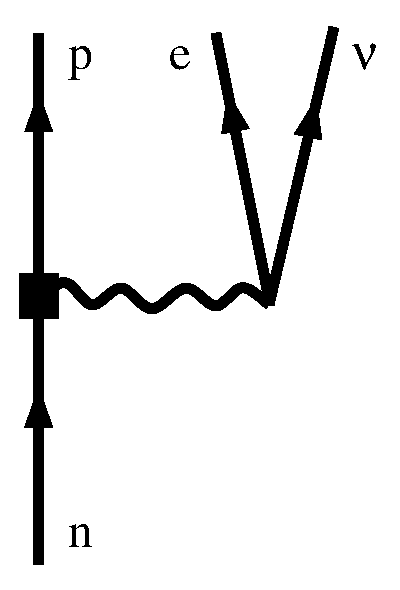
\includegraphics[width=0.16\textwidth]{img/1bc.eps} \hspace{1cm}
			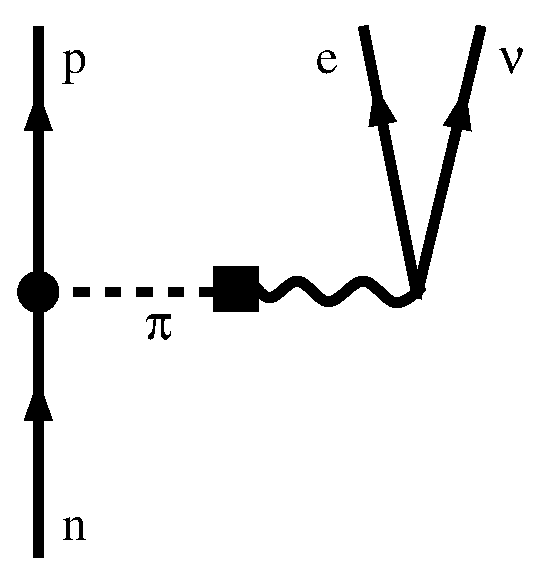
\includegraphics[width=0.22\textwidth]{img/1bc_pion.eps} \\ \vspace{0.5cm}
			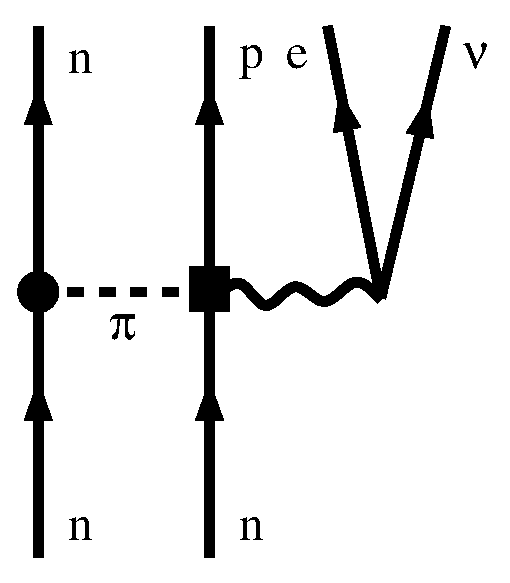
\includegraphics[width=0.22\textwidth]{img/2bc_long.eps} \hspace{.2cm}
			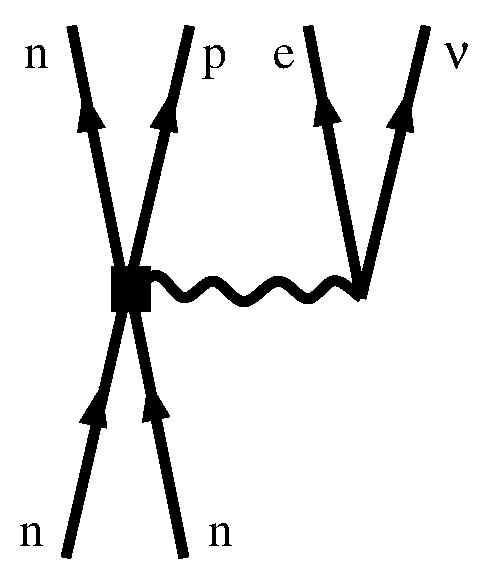
\includegraphics[width=0.21\textwidth]{img/2bc_short.eps} \hspace{.2cm}
   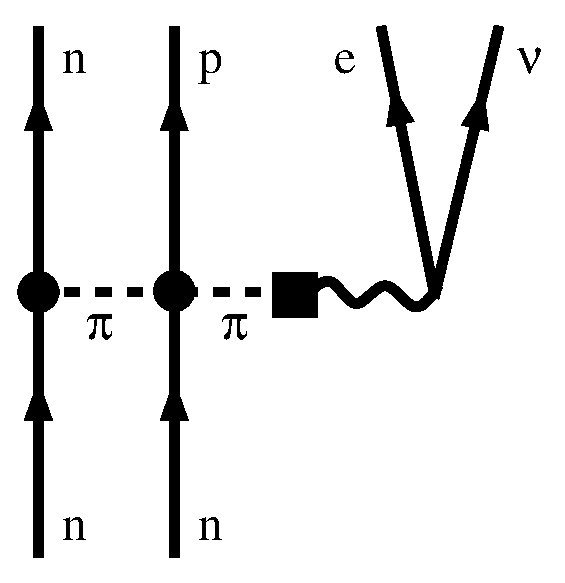
\includegraphics[width=0.245\textwidth]{img/2bc_long_pion.eps}
   \hspace{.2cm} 
   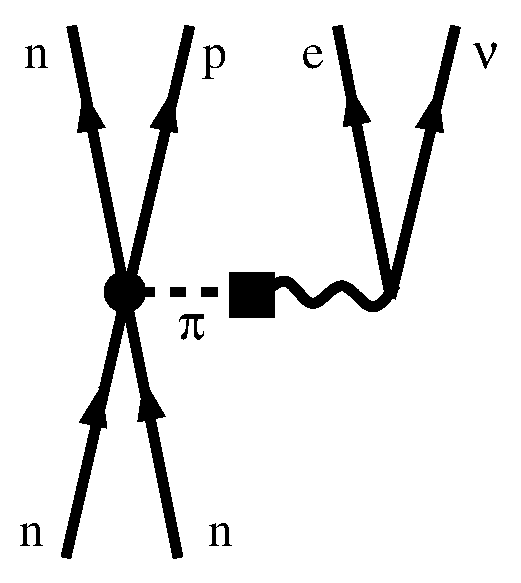
\includegraphics[width=0.225\textwidth]{img/2bc_short_pion.eps}
		\caption{Diagrams for one-nucleon weak-interaction currents (top) and leading two-nucleon weak-interaction currents (bottom). Solid lines represent nucleons, dashed lines indicate pions, and wavy lines the mediator ($W$ boson). In all cases, only one nucleon ($n$) turns into a proton ($p$). The currents with mediator coupling to the pion involve finite momentum transfer, and they are negligible for $\beta$ decay but contribute to $0\nu\beta\beta$ decay. %Vector two-nucleon currents receive contributions from an additional diagram, but they are subleading for $0\nu\beta\beta$ decay.
  \label{fig:currents}}
	\end{center}
\end{figure}

In addition, chiral EFT predicts the leading two-nucleon diagrams that correct one-nucleon currents, indicated in the bottom part of Fig.~\ref{fig:currents}. For $0\nu\beta\beta$ decay, the leading two-nucleon current is the axial one, given by~\cite{Park:2002yp,Krebs:2016rqz,Baroni:2015uza}
\begin{align}
\label{eq:axial2bc}
\bm J_{A,12} &= -\frac{g_A}{F^2_\pi} \, [\tau_1\times\tau_2]^-
\biggl[ 
c_4\Bigl(1-\frac{\bm p}{p^2+m_\pi^2}{\bm p\cdot}\Bigr)
(\bm \sigma_1\times\bm k_2)+\frac{c_6}{4}
(\bm \sigma_1\times \bm p) 
%+i \, \frac{{\bm p_1+\bm p}'_1}{4 m_N}
 \biggr]
\frac{\bm \sigma_2\cdot\bm k_2}{m_\pi^2+k_2^2}  \nonumber \\
&-\frac{2g_A}{F^2_\pi} \,\tau_2^-
\biggl[c_3 \Bigl(1-\frac{\bm p}{p^2+m_\pi^2}{\bm p\cdot}\Bigr) \,\bm k_2+2c_1 m_\pi^2 \frac{\bm p}{p^2+m_\pi^2} \biggr]  \, \frac{
	\bm \sigma_2\cdot\bm k_2}{m_\pi^2+k_2^2}  \nonumber \\
&- 2d_1 \,\tau_1^-  \Bigl(1-\frac{\bm p}{p^2+m_\pi^2}{\bm p\cdot}\Bigr)
\bm \sigma_1 +(1\longleftrightarrow2) \nonumber \\
&- 2d_2 (\tau_1\times\tau_2)^- (\bm \sigma_1 \times \bm \sigma_2)
\Bigl(1-{\cdot \bm p}\frac{\bm p}{p^2+m_\pi^2}\Bigr),
\end{align}
where the final and initial momenta of the nucleons are $\bm k_i=\bm p'_i-\bm p_i$, $\bm p = -\bm k_1-\bm k_2$, and $c_i$ and $d_i$ are couplings of the EFT that need to be determined by fitting to data or from lattice QCD calculations. The terms proportional to the $c_i$'s correspond to the pion-exchange nucleon diagrams in Fig.~\ref{fig:currents}, while those with short-range nucleon interactions enter with the $d_i$'s. Since the chiral EFT couplings also drive nuclear forces, once these are fit, the two-nucleon current in Eq.~\eqref{eq:axial2bc} is entirely predicted. In $0\nu\beta\beta$, a complication arises because the product of two-body currents leads, in general, to a four-body operator hard to handle in many-body calculations. A simple approximation but accurate in $\beta$ decays~\cite{Gysbers:2019uyb}, consists in normal-ordering the two-nucleon current with respect to a Fermi gas reference state with density $\rho_F$. As a result, one obtains an effective one-nucleon current~\cite{Menendez:2011qq}, which just modifies the axial and pseudoscalar terms in Eq.~\eqref{eq:J_nonrel} with corrections $\delta g_A(p^2,c_i,d_i,\rho_F)$ and $\delta g_P(p^2,c_i,d_i,\rho_F)$ dependent on the chiral EFT couplings~\cite{Hoferichter:2020osn}.



Once the weak currents are known, the standard procedure follows second-order perturbation theory to obtain the $0\nu\beta\beta$-decay rate~\cite{Doi:1985dx}. However, this approach misses a relevant contribution only recognized recently, independent to the ones in Eqs.~\eqref{eq:J_nonrel} or~\eqref{eq:axial2bc}. In fact, a chiral EFT analysis shows that, without this additional term, which can be understood as the contribution of high-energy light neutrinos, the decay amplitude is not renormalizable due to the divergences induced by the long-range neutrino potential~\cite{Cirigliano:2018hja}.

\subsubsection{Long-range nuclear matrix elements}

Thus, there are two contributions to the $0\nu\beta\beta$-decay rate. First, the usual long-range part~\cite{Engel:2016xgb}
\begin{align}
\label{eq:nme_full}
  \sqrt{\Gamma_{0\nu\beta\beta}} = & m_{\beta\beta}  \cdot \frac{g_A^2}{R} \cdot    \!\int \!d\bm x \!\int \!d\bm y \;L^{\mu\rho}(\bm x, \bm y) 
  \nonumber \\ & \int \!d\bm p\,e^{i\bm p({\bm x -\bm y})}\cdot 
  \frac{R}{g_A^2} \sum_{n,m}
  \langle 0^+_f\rvert
  \frac{{J}_{L,n}^{\mu\dagger} ({\bm x})\;{J}_{L,m}^{\rho\dagger}({\bm y})}{{ p}^2}
  \lvert 0^+_i\rangle,
\end{align}
where $R=1.2A^{1/3}$ and $g_A^2$ are factorized out for convenience, and $L^{\mu\rho}$ represents the electron currents. The second line in Eq.~\eqref{eq:nme_full} defines the usual long-range NME, which can be written as
\begin{align}
\label{eq:nme}
  M^{0\nu}_\text{long} = \frac{R}{g_A^2}\,
  \langle 0^+_f\rvert
  \sum_{n.m}
  \tau^-_m\tau^-_n \frac{2}{\pi}\int \big[
    &j_0(pr)\,h_F(p^2)\,\mathbb{I}+j_0(pr)\,h_{GT}(p^2)\,{\bm \sigma}_n\cdot{\bm \sigma}_m \nonumber \\
    +&j_2(pr)\,h_T(p^2)\,S_{nm}
    \big]\,d p\,
  \lvert 0^+_i\rangle, %\\
\end{align}
with Fermi (F), Gamow-Teller (GT) and tensor (T) spin structures, $S_{nm}=3({\hat r}\cdot{\bm \sigma}_n)({\hat r}\cdot{\bm \sigma}_m)-{\bm \sigma}_n\cdot{\bm \sigma}_n$, $j_l(pr)$ spherical Bessel functions and $r=\lvert{\bm r}_n-{\bm r}_m\rvert$. The $h_\text{spin}(p^2)$ functions for the long-range NME are
\begin{align}
\label{eq:nu_potentials_explicit}
h_{F}(p^2)&=g_V^2(p^2), \nonumber \\
h_{GT}(p^2)&=g_A^2(p^2)\left[1-\frac{2}{3}\frac{p^2}{p^2+m_\pi^2}+\frac{1}{3}\frac{p^4}{(p^2+m_\pi^2)^2}\right]+g_M^2(p^2)\frac{p^2}{6m_N^2}, \nonumber \\
h_{T}(p^2)&=g_A^2(p^2)\left[\frac{2}{3}\frac{p^2}{p^2+m_\pi^2}-\frac{1}{3}\frac{p^4}{(p^2+m_\pi^2)^2}\right]+g_M^2(p^2)\frac{p^2}{12m_N^2}.
\end{align}
The approximate effect of two-nucleon currents using a normal-ordering approximation can be obtained by modifying the above functions with the corrections $\delta g_A(p^2,c_i,d_i,\rho_F)$ and $\delta g_P(p^2,c_i,d_i,\rho_F)$.

\subsubsection{Short-range nuclear matrix elements}

Second, there is a short-range contribution to the light-neutrino exchange NME, with similar form as Eq.~\eqref{eq:nme_full} but without the neutrino propagator, $1/p^2$. This term does not stem from the product of two currents. It leads to a short-range NME with Fermi-type spin form~\cite{Cirigliano:2019vdj}:
\begin{align}
\label{eq:nme_short}
  M^{0\nu}_\text{short} = \frac{R}{g_A^2}\,
  \langle 0^+_f\rvert
  \sum_{n.m}
  \tau^-_m\tau^-_n \frac{2}{\pi}\int
    &j_0(pr)\,h_S(p)\,p^2\,d p\,\mathbb{I}\,
  \lvert 0^+_i\rangle, %\\
\end{align}
where the function $h_S(p)$ is
\begin{align}
\label{eq:nu_potentials_short}
h_{S}(p)&=2\,g^\text{NN}_\nu f(p/\Lambda_S),
\end{align}
with $g^\text{NN}_\nu$ the corresponding hadronic coupling for this term, and $f(p/\Lambda)$ a function with regulator $\Lambda_S$. Notice that $g^\text{NN}_\nu$ enters linearly in Eq.~\eqref{eq:nu_potentials_short}, in contrast to  any other couplings in  Eq.~\eqref{eq:nu_potentials_explicit}. This indicates that the short-range NME cannot be expressed as a product of two currents. Also, the $p^2$ dependence in Eq.~\eqref{eq:nme_short} illustrates the short-range nature of this NME contribution. Overall, the NME for light-neutrino exchange in Eq.~\eqref{eq:master} is
\begin{align}
M^{0\nu}_\text{light}=M^{0\nu}_\text{long}+M^{0\nu}_\text{short}\,.
\label{eq:nme_total}
\end{align}

Unlike other hadron couplings, $g^\text{NN}_\nu$ cannot be obtained from experiment, because this would involve data on an $2n\rightarrow2p+2e$ decay, or an equivalent process. In principle, the value of the coupling could be extracted from lattice QCD calculations, and efforts in this direction are in progress~\cite{Davoudi:2020gxs,Davoudi:2021noh}. For the time being, approximate QCD results based on dispersion relations~\cite{Cirigliano:2020dmx,Cirigliano:2021qko} and large number of colors~\cite{Richardson:2021xiu} give consistent values for $g^\text{NN}_\nu$ with a reasonable $\sim30\%$ uncertainty. Another strategy is to approximate $g^\text{NN}_\nu$ from the charge-symmetry breaking term of nuclear Hamiltonians~\cite{Cirigliano:2019vdj}. This assumes that the two underlying couplings leading to $g^\text{NN}_\nu$ are the same, as only one of them can of them be constrained from charge-symmetry breaking.

\begin{figure}[t]
	\begin{center}
	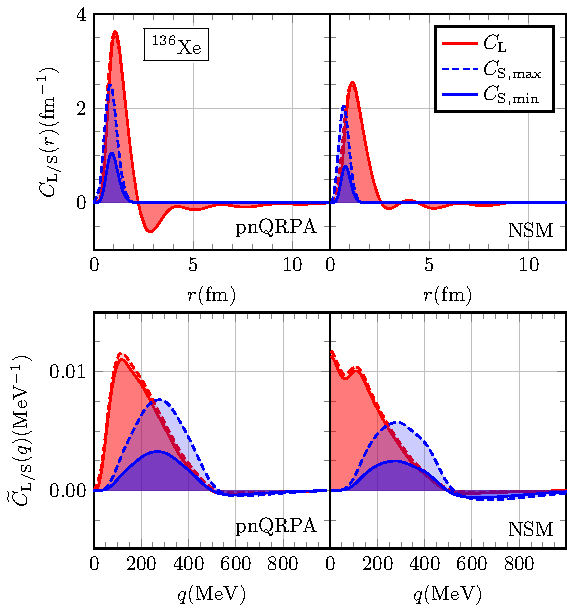
\includegraphics[width=0.65\textwidth]{img/136Xe-QRPA-NSM.pdf}
	\caption{Radial (top panels) and momentum (bottom panels) distributions of the two components of the $0\nu\beta\beta$-decay NME in Eq.~\eqref{eq:nme_total}, calculated for $^{136}$Xe. Red (blue) regions represent the long-range (short-range) NME parts. The left panels show results for the QRPA, and right panels for the nuclear shell model (NSM). Figure with results from Ref.~\cite{Jokiniemi:2021qqv}. \label{fig:NME_density}}
\end{center}
\end{figure}

Figure~\ref{fig:NME_density} shows the radial and momentum distributions of the long- and short-range NMEs for the decay of $^{136}$Xe, calculated by the nuclear shell model and quasiparticle random-phase approximation (QRPA) methods fixing $g^\text{NN}_\nu$ from the charge-symmetry breaking of various Hamiltonians. The NME distributions satisfy
\begin{align}
M^{0\nu}_{\text{long/short}}=&\int C_{L/S}(r)\, d r\,, \\
M^{0\nu}_{\text{long/short}}=&\int \widetilde{C}_{L/S}(p)\, d p\,.
\end{align}
The upper panels in Fig.~\ref{fig:NME_density} highlight that the short-range NME distributions, in blue, actually receive contributions from two decaying nucleons at shorter relative distances than the long-range NME ones, shown in red. Consistently, the lower panels in Fig.~\ref{fig:NME_density} reveal that the short-range NME are dominated by larger momentum transfers. Moreover, Fig.~\ref{fig:NME_density} shows that while the short-range NME is generally smaller than the long-range one, it is a sizeable correction, as expected by chiral EFT.




\subsection{Different nuclear structure approaches}
\label{subsec:manybody}

The nuclear structure of the initial and final nuclei in the $0\nu\beta\beta$ decay plays a relevant role in the value of the NMEs. This is because the relevant momentum transfers in $0\nu\beta\beta$ decay are of the order $p\sim200$~MeV  ---see Fig.~\ref{fig:NME_density}---, comparable to the Fermi momentum, which sets the typical scale of the momenta of nucleons in nuclei. Therefore, a good description of the initial and final nuclei is a necessary condition in order to get reliable NMEs.

\subsubsection{Tests of nuclear structure calculations and {\it $g_A$ quenching}}

All nuclear many-body methods used to study $0\nu\beta\beta$ decay make a significant effort to describe with high quality the structure of the initial and final nuclei. In particular, the low-energy spectrum and electromagnetic transitions are typically well described in shell-model~\cite{Menendez:2009xa,Horoi:2015tkc,Iwata:2016cxn,Coraggio:2020hwx,Coraggio:2022vgy,Tsunoda:2023fqw}, energy-density functional theory~\cite{Yao:2021wst}, interacting boson model~\cite{Kotila:2016pib} and QRPA~\cite{Gimeno:2023dxx} calculations, the standard approaches used to calculate NMEs. More recently, {\it ab initio} or first principles methods, discussed in detail in Sec.~\ref{sec:ab_initio}, have also produced NMEs. In medium-mass nuclei, ab initio methods can match the nuclear structure description of the more phenomenological approaches~\cite{Yao:2020olm,Novario:2020dmr,Belley:2020ejd}, while heavier systems are more challenging~\cite{Belley:2020ejd}.
%
Nuclear structure data is very useful to improve many-body calculations, and therefore NME predictions. Notable examples are nucleon-removal and -addition~\cite{Freeman:2012hr,Freeman:2017bak,Szwec:2016fxr} and charge-exchange~\cite{Frekers:2018edj} reactions involving initial and final $\beta\beta$ nuclei. Novel nuclear structure data keep testing calculations. For instance, a recent measurement of the low-energy spectrum of $^{136}$Cs favors particular shell-model Hamiltonians~\cite{Rebeiro:2023kvs}. In addition, correlation between $0\nu\beta\beta$-decay and other observables can provide insights to the $0\nu\beta\beta$-decay NMEs: good theoretical correlations have been found with double Gamow-Teller~\cite{Shimizu:2017qcy,Yao:2022usd,Jokiniemi:2023bes}, second-order electromagnetic~\cite{Romeo:2021zrn,Jokiniemi:2023bes} and $2\nu\beta\beta$-decay matrix elements~\cite{Jokiniemi:2022ayc}.

However, most calculations systematically overestimate $\beta$-decay Gamow-Teller matrix elements. This puzzle is sometimes coined as {\it $g_A$ quenching}, because matrix elements enter the half-life multiplied by the coupling $g_A$,
\begin{align}
\left(T_{1/2}^\beta\right)^{-1} =  G_{\beta}\left(g_A\,M^{\beta}_{GT}\right)^2\,,
\label{eq:beta}
\end{align}
and the disagreement could also be solved by a reduced $g_A$ value. Fortunately, a simple correction to the $\beta$-decay matrix elements suffices to reach good agreement with data. In shell-model calculations for nuclei with mass number $A\sim10-50$, the matrix-element reduction is captured by constant {\it quenching} factors $q\sim 0.7-0.8$~\cite{Chou:1993zz,Wildenthal:1983zz,Martinez-Pinedo:1996zvt}. Once this factor is known from $\beta$ decays, calculated Gamow-Teller strength distributions agree well with measured values from charge-exchange reactions. Moreover, shell-model half-life predictions for the $2\nu\beta\beta$ decay of $^{48}$Ca~\cite{Caurier:1990dc,Poves:1995rg} and the $2\nu$ double-electron capture of $^{124}$Xe~\cite{CoelloPerez:2018ghg} anticipated the subsequent measured values~\cite{Balysh:1996vr,XENON:2019dti}. The interacting boson model and QRPA also overestimate Gamow-Teller matrix elements~\cite{Barea:2015kwa,Pirinen:2015sma}. The latter, however, by an amount depending on the strength of the proton-neutron pairing interaction used.

Nonetheless, the phenomenological quenching correction, while useful, does not pinpoint the origin of the deficiency in the many-body calculations. A proper answer is given by ab initio methods. These approaches describe the low-energy properties of light systems with $A\lesssim 14$ extremely well, including $\beta$-decay half-lives without any adjustments~\cite{Pastore:2017uwc,Gysbers:2019uyb}. There are two main aspects that ab initio methods incorporate but others do not: first, additional nuclear correlations due the more sophisticated many-body approach; second, two-nucleon currents, introduced in Sec.~\ref{subsec:nme_parts}. In $A\lesssim 14$ nuclei, nuclear correlations are the main aspect to describe well $\beta$ decays~\cite{Pastore:2017uwc,King:2020wmp}, while in heavier systems with $A\sim50-100$~\cite{Gysbers:2019uyb}, both nuclear correlations and two-nucleon currents are needed to reproduce data without any quenching factor. Due to their ability to capture complex correlations and the successful description of $\beta$ decays, ab initio methods promise reliable $0\nu\beta\beta$ NMEs.

\subsubsection{Ab initio methods}
\label{sec:ab_initio}

Ab initio or first principles nuclear structure studies have experienced an exponential boost over the last decade~\cite{Hergert:2020bxy,Ekstrom:2022yea}. In contrast to other many-body approaches which have some phenomenological components, ab initio methods consider all nucleons in the nucleus and use unadjusted nuclear Hamiltonians ---in most cases derived  from chiral EFT. Moreover, the calculations are systematically improvable and the convergence of the results can be checked explicitly.

Since $0\nu\beta\beta$ searches focus on relatively heavy isotopes, ab initio methods like quantum Monte Carlo or the no-core shell model, whose computational cost scales exponentially with the number of nucleons, are limited to benchmark NMEs in light nuclei not relevant for experiments~\cite{Pastore:2017ofx,Basili:2019gvn,Yao:2020olm}. Nonetheless, benchmarks are key to test other approaches suitable for heavier systems.

Three ab initio methods have been used to study the $0\nu\beta\beta$ decay of $^{48}$Ca. Two of them are versions of the in-medium similarity renormalization group (IMSRG), which is based on unitary transformations that bring the many-body Schrodinger equation to a more convenient form~\cite{Hergert:2015awm}. Operators such as the $0\nu\beta\beta$-decay one transform consistently, a feature missed by other many-body methods because of their phenomenological character. The first ab initio NME calculation used the in medium generalized coordinate method (IM-GCM)~\cite{Yao:2020olm}. This variant considers various reference states, as the initial and final $0\nu\beta\beta$ decay nuclei are different, and then includes additional nuclear correlations, exploring deformation  or proton-nucleon pairing via the GCM.

The second is the related valence-space IMSRG (VS-IMSRG) method, which performs IMSRG transformations that decouple a valence space from the core and high-energy orbitals of the full space~\cite{Stroberg:2019mxo}. This is, the VS-IMSRG transforms the many-body problem into one that can be solved with standard nuclear shell-model techniques, with the advantage that it provides an unadjusted nuclear Hamiltonian and a consistent $0\nu\beta\beta$-decay operator.

The third is the the coupled clusters approach, which adds singles (one-particle--one-hole like), doubles (two-particle--two-hole) or triples correlations on top a reference state, which needs to be a reasonable approximation to the nucleus of study~\cite{Hagen:2013nca}. Only recently the CC has been extended to deformed nuclei such as $^{48}$Ti, because the breaking of rotational symmetry is computationally expensive~\cite{Novario:2020dmr}.

The IM-GCM, VS-IMSRG and coupled clusters long-range NMEs for $^{48}$Ca agree within the uncertainties of each many-body method (green bands in Fig.~\ref{fig:NME_long}). Moreover, because of the connection to the shell model, the VS-IMSRG predicts NMEs for most relevant $\beta\beta$ nuclei, see Figs.~\ref{fig:NME_long} and~\ref{fig:NME_full}. For these results, the theoretical uncertainties are dominated by the use of various chiral EFT Hamiltonians. Unlike $\beta$-decay calculations, ab initio $0\nu\beta\beta$-decay NMEs do not include two-nucleon currents yet, because they are more challenging to implement for finite momentum transfer.

\subsubsection{Many-body approaches for heavy nuclei}
\label{sec:maybody_phen}

\begin{figure}[t]
	\begin{center}
	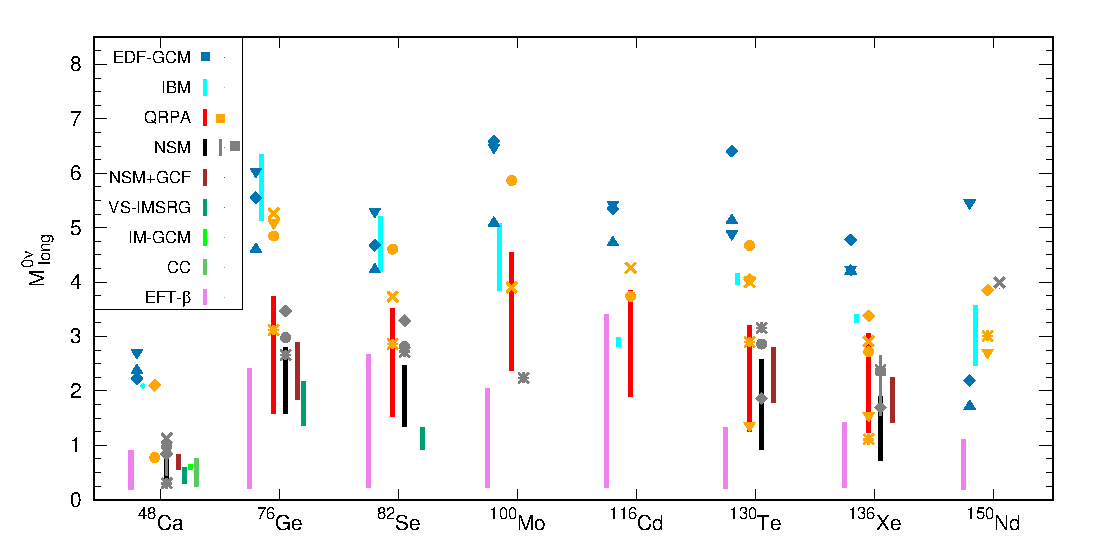
\includegraphics[width=1.02\textwidth]{img/nme_2023.eps}
	\caption{Comparison of the long-range part of the $0\nu\beta\beta$-decay NME for the light-neutrino exchange mechanism, calculated by different many-body methods. For the same method, different symbols indicate results obtained by different groups with different assumptions. Results obtained with energy density functional theory plus the GCM~\cite{Rodriguez:2010mn,LopezVaquero:2013yji,Yao:2014uta} (EDF-GCM, dark blue symbols), the interacting boson model~\cite{Barea:2015kwa,Deppisch:2020ztt} (IBM, cyan bars), the QRPA~\cite{Hyvarinen:2015bda,Simkovic:2018hiq,Mustonen:2013zu,Fang:2018tui,Terasaki:2014rba,Terasaki:2019rbu,Terasaki:2020ndc,Jokiniemi:2022ayc} (orange symbols and red bars), the nuclear shell model~\cite{Horoi:2015tkc,Iwata:2016cxn,Menendez:2017fdf,Horoi:2022ley,Horoi:2023uah,Coraggio:2020hwx,Coraggio:2022vgy,Tsunoda:2023fqw,Jokiniemi:2022ayc} (NSM, grey bars and symbols and black bars), the NSM complemented with the generalized contact formalism~\cite{Weiss:2021rig} (NSM+GCM, brown bars), the IM-GCM~\cite{Yao:2020olm} and VS-IMSRG~\cite{Belley:2020ejd} (dark and light green bars, respectively), the coupled clusters method~\cite{Novario:2020dmr} (CC, green bar), and an EFT of $\beta$ decay~\cite{Brase:2021uny} (EFT-$\beta$, violet bars). See the text for the differences between the calculations and for an explanation of the error bars of each method. \label{fig:NME_long}}
\end{center}
\end{figure}

Among other methods, the nuclear shell model is one of the main workhorses of nuclear structure~\cite{Caurier:2004gf,Otsuka:2018bqq,Brown:2001zz}. It solves the many-body problem in a configuration space around the Fermi surface, using Hamiltonians with a phenomenological component ---in contrast to the VS-IMSRG.
%, usually limited to the part driving the single-particle physics.
Two strategies quantify shell-model NME uncertainties. First, a statistical variation of all elements of shell-model Hamiltonians to obtain NME density distributions for $^{48}$Ca and $^{136}$Xe~\cite{Horoi:2022ley,Horoi:2023uah} (grey bars in Fig.~\ref{fig:NME_long}). Second, systematic calculations in dozens of nuclei exploiting the correlation between $0\nu\beta\beta$ and $2\nu\beta\beta$ NMEs, and $2\nu\beta\beta$ data~\cite{Jokiniemi:2022ayc} (black bars in Fig.~\ref{fig:NME_long}, which include normal-ordered two-body currents). The two $0\nu\beta\beta$ NME extend the range of previous shell-model NMEs (grey symbols).

A hybrid approach can introduce into the shell model additional correlations captured by more sophisticated ab initio calculations. In particular, the generalized contact formalism~\cite{Weiss:2016obx}, combines the short-range correlations captured by the quantum Monte Carlo approach with the shell model~\cite{Weiss:2021rig}. As a result, NMEs are reduced (brown bars in Fig.~\ref{fig:NME_long}) by a larger amount than previous short-range correlations parameterizations~\cite{Simkovic:2009pp}.

The QRPA
%was the first many-body method to describe $\beta\beta$ decays~\cite{Vogel:1986nj,Engel:1988au} and
works in a larger configuration space than the nuclear shell model, albeit with limited nuclear correlations. Most calculations use a spherical QRPA on top of G-matrices~\cite{Hyvarinen:2015bda,Simkovic:2018hiq}, but they can accommodate deformation~\cite{Fang:2018tui} or energy-density functionals~\cite{Mustonen:2013zu}. The QRPA NME uncertainty has been explored with systematic calculations varying the proton-neutron pairing interaction and using the $0\nu\beta\beta-2\nu\beta\beta$ NME correlation~\cite{Jokiniemi:2022ayc} (red bars in Fig.~\ref{fig:NME_long}). The corresponding NME range is smaller than other QRPA values (orange symbols) because of including normal-ordered two-body currents.

Energy-density functional theory combined with the GCM is the other workhorse of nuclear structure studies, especially for heavy nuclei or high-energy excitations~\cite{Paar:2007bk,Robledo:2018cdj}. Different calculations use nonrelativistic~\cite{Rodriguez:2010mn,LopezVaquero:2013yji}
or relativistic~\cite{Yao:2014uta} functionals (dark blue symbols in Fig.~\ref{fig:NME_long}).

The interacting boson model is an algebraic approach assuming nuclei formed by bosons~\cite{Iachello:2006fqa} coupled to different angular momentum. Boson degrees of freedom are then mapped to fermions. For NMEs, the uncertainties explored comprise two interacting boson model Hamiltonians fitted to different properties of the initial and final nuclei~\cite{Barea:2015kwa,Deppisch:2020ztt} (cyan bars in Fig.~\ref{fig:NME_long}).

Finally, $0\nu\beta\beta$ decay can be studied by a nuclear effective theory for $\beta$ and $\beta\beta$ decays which considers spherical nuclei with nucleon particles or holes attached~\cite{CoelloPerez:2017xsq,Brase:2021uny}. The coupling of the EFT is fitted using the shell-model $0\nu\beta\beta-2\nu\beta\beta$ NME correlation~\cite{Shimizu:2017qcy}, as the EFT can predict $2\nu\beta\beta$ NMEs. The theoretical uncertainties are predicted by the EFT, with the violet bars in Fig.~\ref{fig:NME_long} showing leading-order uncertainties.

\subsection{Nuclear matrix elements with theoretical uncertainties}
\label{subsec:nme_current}

Figure~\ref{fig:NME_long} compares predictions for the long-range part of the $0\nu\beta\beta$-decay NME from all nuclear many-body methods discussed in Secs.~\ref{sec:ab_initio} and \ref{sec:maybody_phen}. These sections also explain in detail the meaning of of the error bars in Fig.~\ref{fig:NME_long} for each many-body calculation. We note that all theoretical uncertainties are underestimated, being the one for the EFT for $\beta$ decay the one closer to the complete error ---however, these NMEs are also based on shell-model NME correlations, see Sec.~\ref{sec:maybody_phen}.
%This comprises NMEs from several many-body methods beyond the ones available about a decade ago, which limited to the shell model, QRPA, energy-density functional theory and interacting boson model.

Most predicted NME values cluster around $M^{0\nu}_\text{long}\sim1-3$ for the majority of isotopes. These are similar, or even smaller values than the lower-end NMEs available a decade ago~\cite{Gomez-Cadenas:2010zcc}, which roughly correspond to the shell-model results in Fig.~\ref{fig:NME_long} (grey symbols and bars). {\it This reduction in the NME values appears because many of the recent calculations address, at least partly, the causes of the $g_A$ quenching in $\beta$ decays}. Therefore, a significant part of the reduction of the NME values due to this issue is expected to be already captured in the NMEs shown in Fig.~\ref{fig:NME_long}.

This is, modern calculations that bring additional aspects, in the form of ab initio NME results (green bars with three different tones), short-range correlations introduced by the generalized contact formalism (brown bars), normal-ordered two-nucleon currents (black and red bars), and the EFT for $\beta$ decay (violet bars) all suggest relatively small NME values. This is especially clear for the $^{48}$Ca long-range NME, where the three different ab initio and several other methods agree within uncertainties. Only energy-density functional GCM and interacting boson results (dark blue symbols and cyan bars) point to relatively large NME values, for $^{48}$Ca and for other isotopes. The latter results, however, may be overestimated because of not including explicit proton-neutron pairing correlations or high-seniority components~\cite{Menendez:2014ena,Hinohara:2014lqa,Menendez:2015kxa}. Some QRPA NMEs without two-nucleon currents (orange symbols) also prefer larger NME values than most many-body methods. 

\begin{figure}[t]
	\begin{center}
	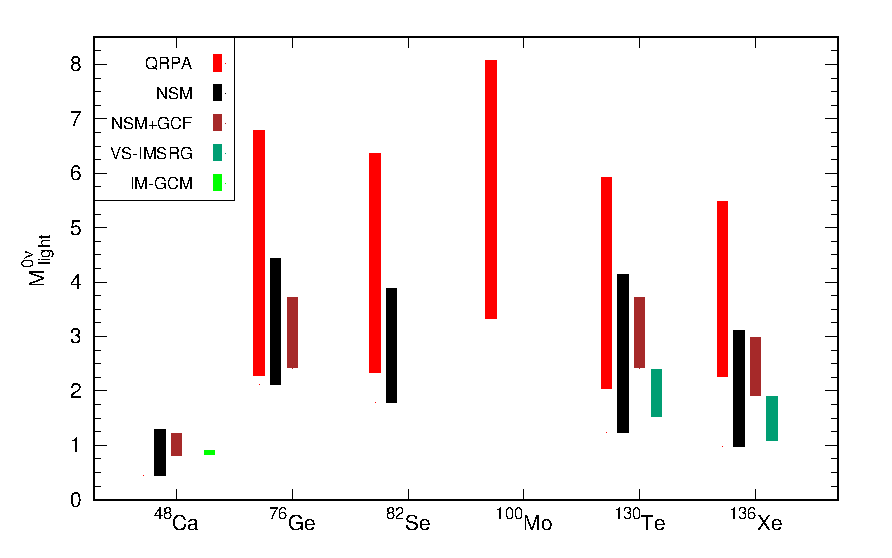
\includegraphics[width=0.8\textwidth]{img/nme_total_2023.eps}
	\caption{Comparison of the full $0\nu\beta\beta$-decay NME for the light-neutrino exchange mechanism, calculated with different many-body methods: the QRPA~\cite{Jokiniemi:2022ayc} (red bars), nuclear shell model (NSM, black bars)~\cite{Jokiniemi:2022ayc}, NSM with generalized contact formalism~\cite{Weiss:2021rig} (NSM+GCF, brown bars), VS-IMSRG~\cite{Belley:2023btr} (dark-green bars) and IM-GCM~\cite{Wirth:2021pij} (light-green bar). The color code is the same as in Fig.~\ref{fig:NME_long}. See the text for the differences between calculations and for an explanation of the error bars of each method.\label{fig:NME_full}
	}
\end{center}
\end{figure}

However, Eq.~\eqref{eq:nme_total} indicates that the NMEs shown in Fig.~\ref{fig:NME_long} are only a part of the total NMEs for $0\nu\beta\beta$ decay mediated by the light-neutrino exchange. Figure~\ref{fig:NME_full} compares the predictions for the total NMEs of the few many-body methods which so far have performed dedicated short-range NME calculations. Like in Fig.~\ref{fig:NME_long}, the total NMEs in Fig.~\ref{fig:NME_full} include part of the causes responsible for the $g_A$ quenching in $\beta$ decays, especially the additional correlations introduced by ab initio methods or the two-nucleon currents included into the shell model and QRPA results.

Light- and dark-green bars in Fig.~\ref{fig:NME_full} show ab initio IM-GCM and VS-IMSRG NMEs, which include nuclear correlations key to reproduce $\beta$-decay data. The small IM-GCM uncertainty bar only takes into account the error due to the short-range coupling $g^{\text{NN}}_\nu$, while the larger VS-IMSRG bars are dominated by the uncertainties due to three nuclear Hamiltonians used. Two of the other results in Fig.~\ref{fig:NME_full} incorporate missing aspects to standard shell-model calculations, either short-range physics via the generalized contact formalism (brown bars) or with normal-ordered two-nucleon currents (black bars). The latter have wider uncertainties because they consider $g^{\text{NN}}_\nu$ values from various nuclear Hamiltonians ---this strategy has larger uncertainty than the one used by ab initio methods--- and also because it is based on systematic calculations to gauge statistical shell-model uncertainties. These four calculations give consistent NME values for all available isotopes. The QRPA NMEs (red bars), while generally consistent with other results, extend to larger values and present larger uncertainties. Like in the shell model, these are dominated by systematic calculations to estimate statistical uncertainties and the value of $g^{\text{NN}}_\nu$.



\section{Ingredients for the ultimate neutrinoless double beta decay experiment} \label{sec:ingredients}
%%%%%%%%%%%%%%%%%%%%%%%%%%%%%%%%%%%%%%%%%%%%%%%%%%%%%%%%%%%%%%%%%%%%%%%%%%%
%The discovery of \bbonu\ would represent a substantial breakthrough in particle physics. A single, unequivocal observation of the decay would prove the Majorana nature of neutrinos and the violation of lepton number. Alas, that is not, by any means, an easy task. The design of a detector capable of identifying efficiently and unambiguously such a rare signal represents a major experimental challenge.

%Given the sensitivity to $T_{1/2}^{0\nu}$ already achieved, the first ingredient required for the next generation of \bbonu\ experiment is a 
%To start with, one needs a
 %large mass of a suitable (and always scarce) \bb\ isotope in order to probe in a reasonable time the extremely long lifetimes expected. 
% For instance, for a Majorana neutrino mass of 18 meV, corresponding to the lowest possible \mbb\ value in the inverted ordering scenario (see fig.~\ref{fig:mbetabetavsmlight}), it can be estimated using eq.~(\ref{eq:Tonu}) and a sound assumption for the NMEs that half-lives in the range of $10^{27}$--$10^{28}$ years must be explored (\textit{i.e.}, at least 17 orders of magnitude longer than the age of the universe!). 
 %A better sense of what such extremely long half-lives mean can be grasped with a 
 %
 %This can be easily illustrated with a simple calculation. 
Consider the radioactive decay law in the approximation $T_{1/2}\gg t$, where $t$ is the exposure time. Assuming a hypothetical \bbonu\ process with a half-life $T_{1/2}^{0\nu}$, the expected number of \bbonu\ events in an experiment is given by
%
\begin{equation}
N_{\bbonu} = \log 2 \ \frac{\Mbb\cdot N_{A}}{W_{\beta\beta}}  \frac{t}{T_{1/2}^{0\nu}}, 
\label{eq:Nbb}
\end{equation}
%
where \Mbb\ is the mass of the \bb\ emitting isotope,\footnote{Note that our notation in eq.~(\ref{eq:Nbb}), and in the rest of this review, differs from the usually adopted one, derived from source-equals-detector experimental configurations. In the source-equals-detector notation, one refers to the total active mass $M$ of the detector, which is related to the mass \Mbb\ of the \bb\ isotope via the following relationship:
%
\begin{equation}
\Mbb\ = W_{\beta\beta}\cdot \frac{M}{W}\cdot a\cdot \eta ,
\label{eq:mbbversusm}
\end{equation}
%
where $W$ is the molecular weight of the molecule of the active material, $a$ is the isotopic abundance of the candidate \bbonu\ nuclide, and $\eta$ is the number of \bbonu\ element nuclei per molecule of the active mass. For example, TeO$_2$ bolometric detectors with a natural isotopic abundance in \Te{130} are characterized by $W_{\beta\beta}=129.9\ \mathrm{g/mol}$, $W=159.6\ \mathrm{g/mol}$, $a=0.34167$ and $\eta=1$, such that $\Mbb = 0.278 M$. To stress this somewhat unconventional mass notation and to avoid any confusion, we will make use in the following of \kgbb\ as the mass unit to indicate one kilogram of \bb\ emitter mass. Notice that, in principle the best quantity to express the \bbonu\ exposure, and the background rate per unit exposure and unit energy discussed below, is neither kg$\cdot$year nor \kgbb $\cdot$year, but rather $n_{\beta\beta}\cdot$year, where $n_{\beta\beta}=\Mbb \cdot N_A/W_{\beta\beta}$ is the number of moles of the \bb\ nuclide. To avoid an even more ``radical'' departure from commonly employed units, we stick to \kgbb$\cdot$year units in the following.} 
%
$N_{A}$ is the Avogadro constant and $W_{\beta\beta}$ is the molar mass of the \bb\ isotope.

 %and $\varepsilon$ is the signal detection efficiency.
%\cdot \varepsilon \cdot
Take \Xe{136} as an example, and suppose that 
%that the lifetime of the \bbonu\ process is one order of magnitude larger than current limits, e.g., 
$T_{1/2}^{0\nu}\sim 10^{27}$ year. Assume an ideal apparatus with detection efficiency $\varepsilon =1$ and perfect energy resolution (i.e., all \bbonu\ events pile up in a perfect spike at \Qbb). Such a detector has zero expected background, and then the observation of a single event implies a discovery. Solving eq.~\ref{eq:Nbb} for $ N_{\bbonu}=1$ yields $\Mbb \cdot t \sim 330$ \kgbb~yr. %Suppose that the experiment runs for one year. 
%It follows that an ideal detector with efficiency one and zero background requires an exposure of several hundreds kilogram$\cdot$year of isotope mass (\Mbb) to improve current limits by one order of magnitude. 
Introducing a realistic efficiency $\varepsilon \sim$ 0.3--0.6, one finds $\Mbb \cdot t \sim 0.5$--1~ton~year. It follows that the first ingredient required for the next generation of \bbonu\ experiments is a 
%To start with, one needs a
large mass of a suitable (and always scarce) \bb\ isotope in order to probe in a reasonable time the extremely long half-lives expected. 

%It follows from eq.~(\ref{eq:Nbb}) that, in order to observe (assuming perfect detection efficiency and no disturbing background) as little as one decay per year and assuming a Majorana neutrino mass of 18 meV ($T_{1/2}^{0\nu}\sim 10^{27}$--$10^{28}$ years), masses of \bb\ isotope of the order of one tonne are needed.

In the presence of backgrounds, which we discuss in sections~\ref{subsec:bgrsources} and \ref{subsec:bgrmitigation},  the observation of a single event is not enough to establish a discovery. Imagine now that our \Xe{136} experiment predicts a background of one event per year. Since the process is Poisson distributed, the probability of observing, say, 9 background events when 1 is expected is $\sim 10^{-6}$. Observing 9 events would therefore establish a discovery at roughly 5$\sigma$, that is, roughly equivalent to observing one event in the absence of background. Thus, a single expected background event per year would translate in the need to increase the mass by, essentially, one order of magnitude with respect to the background-free case. The second major ingredient for \bbonu\ experiments, therefore, is to suppress backgrounds as much as possible, given its enormous impact on the sensitivity. 
 %Background suppression is, therefore, essential for a \bbonu\ experiment. We discuss background sources
 %in \ref{subsec:bgr_sources}.
 %
 %The situation becomes even more complicated when considering real experimental conditions. 
% The background processes that can mimic a \bbonu\ signal 
% %in a detector 
% are copious. All the experiments have to deal with an intrinsic background, the \bbtnu\ decay, that can only be distinguished by measuring the energy of the emitted electrons, since the neutrinos escape the detector undetected (see fig.~\ref{fig:modes}). Good energy resolution is therefore essential to prevent the \bbtnu\ spectrum tail from spreading over the \bbonu\ ROI, or to cause pileup (in the case of isotopes with a fast \bbtnu\ mode such as \Mo{100}, the probability of overlapping two simultaneous \bbtnu\ events in a dense crystal is not negligible and in fact in the case of CUPID a leading cause of background).    
 %
 %On the other hand, the kinematics of the reaction results in a vanishing rate of \bbtnu\ events, which decrease roughly with $E^7$, for $E \sim \Qbb$. Thus, the \bbtnu\ mode does not become a leading background up to very long \bbonu\ lifetimes  ($T_{1/2}^{0\nu} \sim 10^{28}$ year) even for a ``modest'' energy resolution of $\sim 3\%$ FWHM, typical of LXe. Instead the sensitivity of large liquid scintillator experiments such as KamLAND-Zen and SNO+, may ultimately be limited by the tail of \bbtnu\ events which enters the ROI due to their relatively poor energy resolution (KamLAND-Zen has achieved so far a resolution $\sim 10\%$ FWHM).
% 
%Energy resolution 
%It is also essential to suppress the continuous background arising from natural radioactivity, cosmic rays (and eventually solar neutrino interactions in the detector active target). 
%Notice that a detector with a perfect energy measurement would suppress all backgrounds, since the signal would be a spike of zero width. Although no such beast has been built yet, germanium calorimeters come pretty close, with a resolution of the order of 0.15 \%. And yet, as shown by the GERDA experiment \cite{GERDA:2020xhi}, additional handles are required to control the backgrounds already for lifetimes of the order of  $10^{26}$ year. 
%  the backgrounds arising from natural radioactivity (with a lifetime at least seventeen order of magnitude faster than the putative signal being sought), and other processes (such as cosmogenic backgrounds) spread up to energies well above the \Ge{76} \Qbb (2039 keV), and, in the absence of further handles may bury the putative, extremely weak signal. 
 %
  %Nevertheless, this \emph{energy signature} could not be enough per se: 
 %a continuous spectrum arising from a variety of other backgrounds can easily overwhelm the signal peak. Other signatures, like particle identification or the observation of the daughter nucleus, are a bonus to provide a robust result against backgrounds. An overview of potential background sources affecting \bbonu\ experiments is given in Sect.~\ref{subsec:bgr_sources}.

Several other factors such as the choice of isotope, detection efficiency or the scalability to large masses must be taken into account as well when choosing the experimental technique. In practice, it is not possible to optimize all of these parameters simultaneously. Different choices have led to a variety of experimental approaches. In order to compare their discovery potential, a figure of merit, the experimental sensitivity to \mbb, is normally used. We discuss it in section~\ref{subsec:sensitivitydefinition}. 
%describe it in Sect.~\ref{subsec:sensitivitydefinition}, followed by a discussion on the main parameters entering this figure (Sect.~\ref{subsec:isotope} to Sect.~\ref{subsec:efficiency}).

%Before moving forward, we note that our notation in eq.~(\ref{eq:Nbb}) --- and in the rest of this review --- differs from the usually adopted one, derived from source-equals-detector experimental configurations. In the source-equals-detector notation, one refers to the total active mass $M$ of the detector, which is related to the mass \Mbb\ in the \bb\ isotope via the following relationship:
%%
%\begin{equation}
%\Mbb\ = W_{\beta\beta}\cdot \frac{M}{W}\cdot a\cdot \eta ,
%\label{eq:mbbversusm}
%\end{equation}
%%
%where $W$ is the molecular weight of the molecule of the active material, $a$ is the isotopic abundance of the candidate \bbonu\ nuclide, and $\eta$ is the number of \bbonu\ element nuclei per molecule of the active mass. For example, TeO$_2$ bolometric detectors with a natural isotopic abundance in \Te{130} are characterized by $W_{\beta\beta}=129.9\ \mathrm{g/mol}$, $W=159.6\ \mathrm{g/mol}$, $a=0.34167$ and $\eta=1$, such that $\Mbb = 0.278 M$.\footnote{To stress this somewhat unconventional mass notation and to avoid any confusion, we will make use in the following of \kgbb\ as the mass unit to indicate one kilogram of \bb\ emitter mass.} \footnote{In principle the best quantity to express the \bbonu\ exposure, and the background rate per unit exposure and unit energy discussed below, is neither kg$\cdot$year nor \kgbb $\cdot$year, but rather $n_{\beta\beta}\cdot$year, where $n_{\beta\beta}=\Mbb \cdot N_A/W_{\beta\beta}$ is the number of moles of the \bb\ nuclide. To avoid an even more ``radical'' departure from commonly employed units, we stick to \kgbb$\cdot$year units in the following.}
%
%%%%%%%%%%%%%%%%%%%%%%%%%%%%%%%%%%%%%%%%%%%%%%%%%%%%%%%%%%%%%%%%%%%%%%%%%

\subsection{Background sources} \label{subsec:bgrsources}
The background processes that can mimic a \bbonu\ signal 
%in a detector 
are numerous. All the experiments have to deal with an intrinsic background, the \bbtnu\ decay, that can only be distinguished by measuring the energy of the emitted electrons, since the neutrinos escape the detector undetected (see fig.~\ref{fig:modes}). Good energy resolution is therefore essential to prevent the \bbtnu\ spectrum tail from spreading over the \bbonu\ region of interest, or to cause pileup (in the case of isotopes with a fast \bbtnu\ mode such as \Mo{100}, the probability of detecting two simultaneous \bbtnu\ events in a dense crystal is not negligible, and in fact in the case of CUPID a leading cause of background).    

Any process generating energy deposits in the detector's active volume of the order of the $Q$ value of the double beta reaction is a potential background in \bbonu\ searches. The background sources can be categorized by their production mechanism, as follows: radiogenic (produced by natural radioactivity), cosmogenic (produced by the action of cosmic rays) and heliogenic (produced by the Sun). They can also be classified by their spatial origin: internal or external to the detector.

The natural radioactivity of detector components is often the main background in \bbonu\ experiments. Even though the half-lives of the natural decay chains are comparable to the age of the Universe, they are very short compared to the half-life sensitivity of \bbonu\ experiments. Therefore, even traces of these nuclides can become a significant background. The energy deposits may be produced directly by the $\alpha$ or $\beta$ particles produced in these decays, as well as from the interactions inside the detector of the nuclear de-excitation $\gamma$ rays from the daughter nuclei produced in the decay. The decays of \Tl{208} and \Bi{214} are particularly pernicious, given the high $Q$ values of these reactions, therefore polluting the energy region of interest of most \bb\ emitters. These isotopes are produced as by-products of the natural thorium and uranium decay chains (see fig.~\ref{fig:decaychain}), and they are present at some level in all materials. The natural radioactivity from the detector surroundings may also be relevant, if this external activity is sufficiently high. This can be the case of laboratory concrete walls and surrounding rock, for example. 
%Beyond natural radioactivity, the two-neutrino double beta decay from the same isotope used for the \bbonu\ search is, of course, another example of a radiogenic, internal, background. 

%%%%%
\begin{figure}[t!b!]
\begin{center}
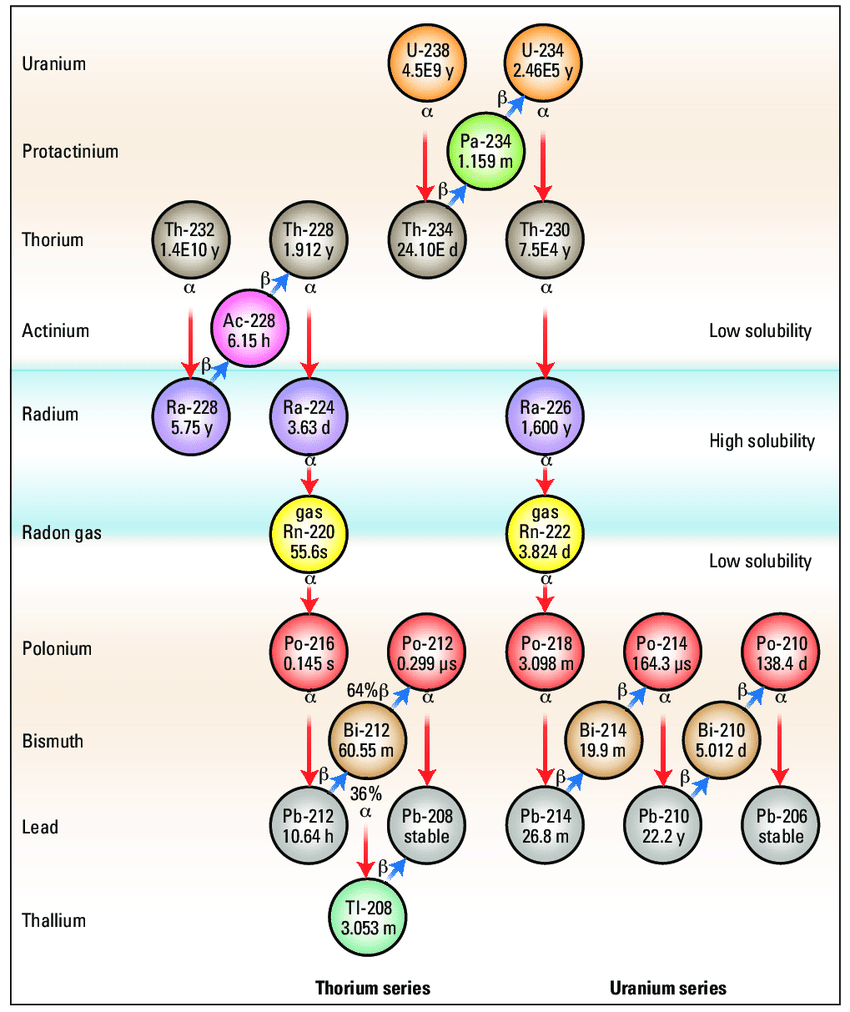
\includegraphics[width=0.8\textwidth]{img/Natural-thorium-and-uranium-decay-chains.png} 
%\vspace*{8pt}
\caption{Natural thorium (left) and uranium (right) decay chains. From \cite{decaychain}.} \label{fig:decaychain}
\end{center}
\end{figure}
%%%%%

Beyond primordial activity, the action of cosmic rays on detector targets and materials may also activate isotopes that would otherwise be stable. Cosmogenic activation of materials may occur both on the surface, during production, transportation or storage, or even underground, during detector operations. While activation on the surface is mostly due to the flux of cosmic-ray neutrons reaching sea level, the one underground is due to cosmic-ray muons.\footnote{A depth of a few tens of meter water equivalent (m.w.e.) is sufficient to suppress the flux of cosmic-ray nucleons.} In the case of underground activation, cosmic-ray muon interactions can produce nuclear breakup ("spallation"), producing a cascade of fast neutrons and electromagnetic showers as a result. The neutrons eventually thermalize and get captured by other nuclei in/near the detector active volume. The resulting neutron-rich nuclei may be unstable, eventually suffering $\beta$ decay, producing both electrons and gamma-rays. This detector activity may be both prompt ($\lesssim$1~ms time delay) or delayed compared to the original muon interaction.

At the depths of underground laboratories, the only other surviving radiation beyond cosmic-ray muons are neutrinos. Very massive detectors, such as liquid-scintillator calorimeters, suffer from an irreducible external background: the solar neutrino flux. Solar neutrinos may elastically scatter off electrons in the detector medium to create energy deposits in the \bbonu\ energy region of interest.

%%%%%%%%%%%%%%%%%%%%%%%%%%%%%%%%%%%%%%%%%%%%%%%%%%%%%%%%%%%%%%%%%%%%%%%%%

\subsection{Background mitigation} \label{subsec:bgrmitigation}

%Minimizing the background index, $c$, in $\upsilon_2$, is the main business of 
%\bbonu\ experiments. 
%Double beta decay experiments are mostly about suppressing the background sources mentioned in Sect.~\ref{subsec:bgr_sources}. As we have seen already, the mere presence of background in the region of interest around \Qbb\ changes the regime of the \mbb\ sensitivity from a $(\Mbb \cdot t)^{-1/2}$ dependence to $(\Mbb \cdot t)^{-1/4}$. In the following, we describe the 
%Background mitigation techniques can be separated into {\emph passive} and {\emph active}, depending on whether detector information is used or not. We discuss first the passive techniques, which are common to most experiment. 
%
%Starting with passive mitigation techniques, 

All \bbonu\ experiments must use materials with extremely low amounts of radioactive impurities. Selection, manufacturing, cleaning and installation of detector materials has to be conducted with extreme care, relying on radio-pure protocols at all times. Material selection is based on extensive radio-purity assays of all detector materials, using both gamma spectroscopy and mass spectrometry techniques. Cleaning of detector components is necessary to remove surface contaminants, such as dust or lubricants, from the manufacturing processes. Cleaning is carried out in detergent and acidic solutions, sometimes using ultrasonic techniques. Dedicated manufacturing processes are used to avoid contamination. Detector installation occurs in clean-room conditions. The most stringent radio-purity requirements apply to the detector active target itself, as well as to other massive detector components (e.g., shielding parts) in proximity to it. The new-generation experiments are being fabricated from amazingly radio-pure components, some with specific activities as low as 1 $\mu$Bq/kg or less. Specific activities that are that low require \Th{232} and \U{238} impurities in the bulk materials that are below the part per trillion (ppt) level in mass, $<10^{-12}$~g/g. Ultrapure detector material examples include organic scintillator and xenon fluids through closed-loop re-circulation and purification systems, 2,000-year-old Roman shielding lead, and fabrication of ultrapure shielding copper via electroforming techniques.

Beyond primordial activity from contaminants in the natural decay chains, production inside detector materials of radioactive nuclides by cosmic-rays may also occur. Cosmogenic activation is, of course, more severe on surface. Therefore, for experiments using materials that can get activated (like germanium-based experiments), underground fabrication and storage of the detector components is essential.

Radon gas, particularly \Rn{222}, is an intermediate by-product of the natural decay chains, that also needs to be suppressed inside and near \bbonu\ experiments. Being gaseous, radon does not stay trapped within detector components and may infiltrate inside detector sensitive regions, hence requiring a separate mitigation strategy. Also, radon daughters tend to be electrically charged and stick to surfaces. Concerning airborne radon, most deep underground laboratories have radon abatement systems capable of suppressing the radon concentration in the air by several orders of magnitude, down to 1 mBq/m$^3$ concentrations, providing effectively radon-free air in the vicinity of the detectors. The flushing of pure nitrogen gas is an equally effective, although more expensive, alternative to provide a radon-free environment. The radon concentration in the air is monitored in real-time at underground locations. Radon may also diffuse inside fluid-based (liquid or gaseous) \bbonu\ detectors, typically via emanation from detector materials. Active filtration systems (radon traps) may be used to mitigate this internal radon component.

Concerning external backgrounds originated outside the detectors, the techniques to passively mitigate them involve placing the experiments at deep underground laboratories, and by enclosing them into shielding systems. 

Deep underground laboratories are research infrastructures with an overburden typically larger than 1000 meters water equivalent (m.w.e.). In general, the depth requirement for a \bbonu\ experiment varies according to the detector technology. A very efficient shielding and additional detection signatures such as topological information can compensate the benefits of a very deep location. Figure \ref{fig:underground_facilities} shows the laboratory depth and size of several underground facilities currently available to host physics experiments around the world. In addition to depth, other important factors characterizing the underground sites include the size of the excavated halls available for science, and the services provided to the experiments. The size is an important factor to take into account, especially for experimental proposals at the ton-scale and beyond, given that some of them need large volumes. The most relevant deep underground laboratories for current and future \bbonu\ experiments, listed in order of decreasing depth, are at the moment: the China Jinping Underground Laboratory (CJPL, China), SNOLAB (Canada), the Gran Sasso National Laboratory (LNGS, Italy), the Sanford Underground Research Facility (SURF, USA), the Kamioka Observatory (Japan) and the Canfranc Underground Laboratory (LSC, Spain). For a recent review of the currently available underground facilities around the world, see reference \cite{Ianni:2023fvs}. 

%%%%%
\begin{figure}[t!b!]
\begin{center}
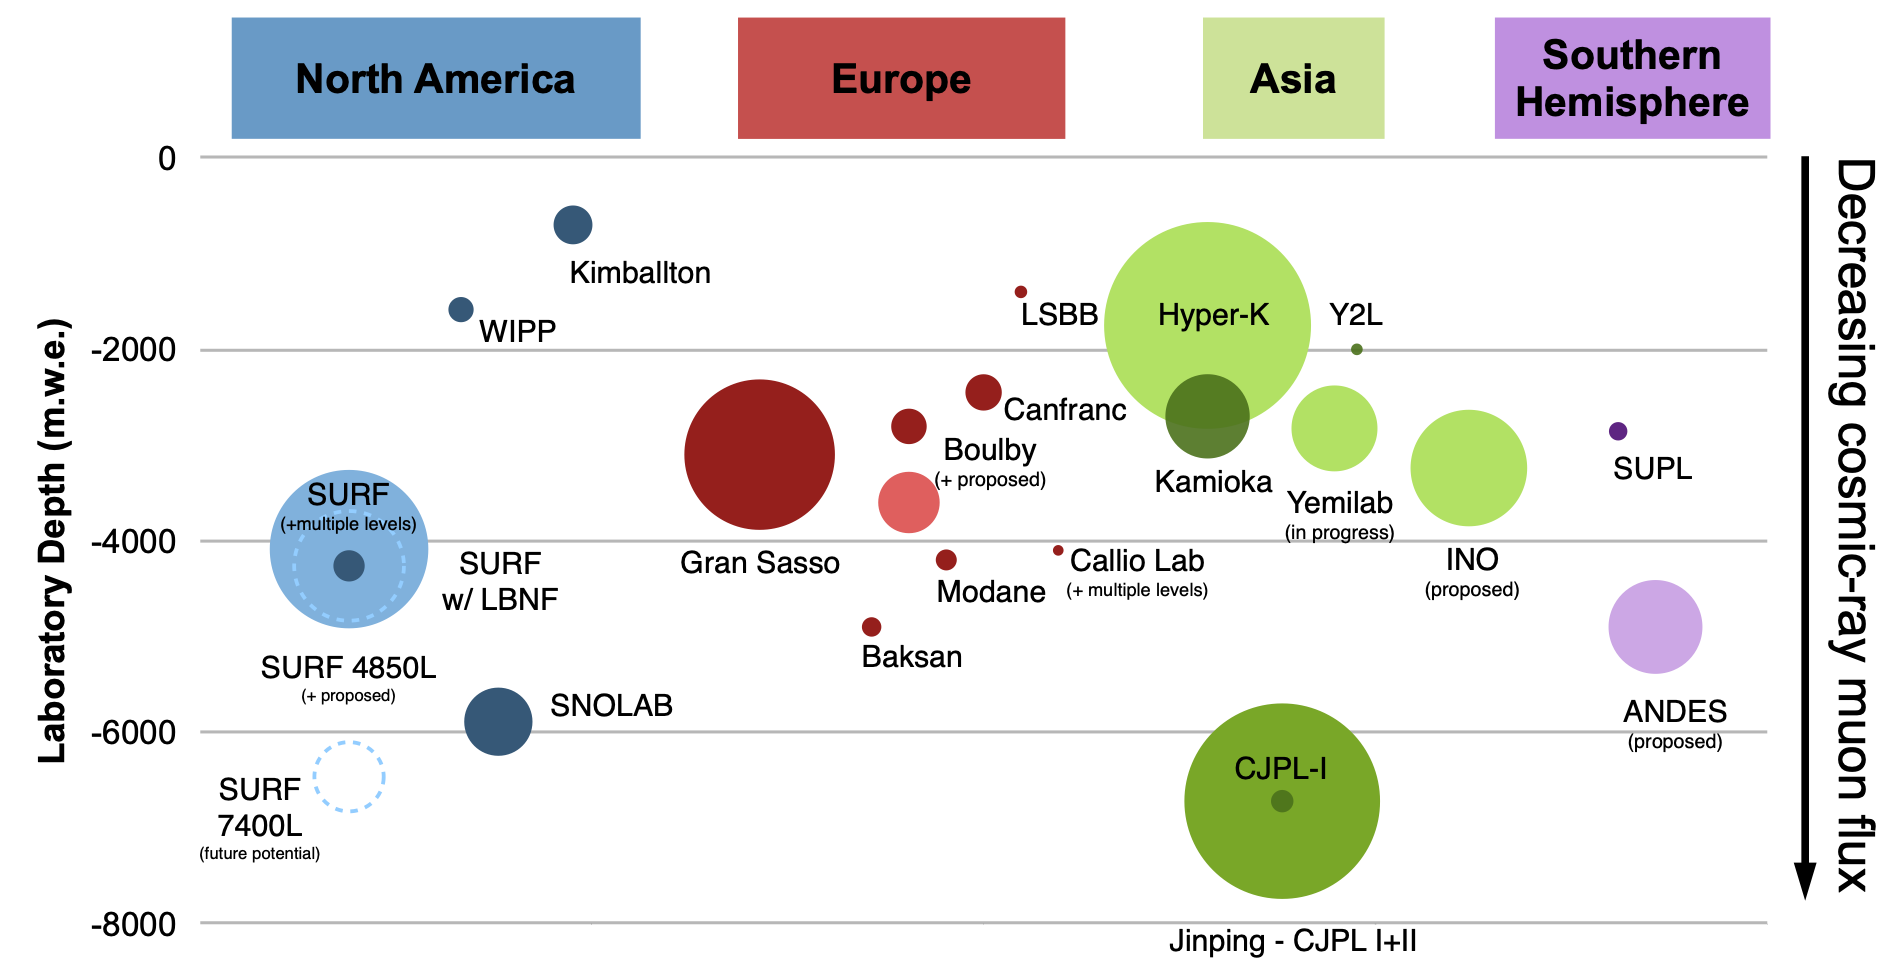
\includegraphics[width=\textwidth]{img/UndergroundFacilities.png}
%\vspace*{8pt}
\caption{\label{fig:underground_facilities}Overview of underground facilities located around the world. The size (volume of science space) and effective shielding depth (total muon flux) are shown. Some muon flux values are estimated using a recent parameterization \cite{JNE:2020bwn}. Figure from \cite{Baudis:2022pzb,Heise:2022iaf}.}
\end{center}
\end{figure}
%%%%%

Shielding systems surrounding the detectors are another very effective technique to passively suppress external backgrounds. As such, they are used ubiquitously in \bbonu\ experiments. In the design of a shielding system against external backgrounds, a \emph{graded shielding} principle is followed: the thickness of a shield component does not need to reduce the flux below the contribution of the next inner component, with the innermost shield component selected to be the radiopurest.

Despite their sizable penetrating power, external neutrons from cosmic-ray interactions and from $(\alpha$,n) reactions can be shielded with layers of hydrogenous material. On the other hand, the external $\gamma$-ray flux produced by radioactive decays in the rock of the underground cavern can be suppressed via dense, high $Z$, radiopure materials such as lead and copper. 


\subsection{Sensitivity of a \bbonu\ experiment} \label{subsec:sensitivitydefinition}

%All \bbonu\ experiments have to deal with non-negligible backgrounds, an only partially efficient \bbonu\ event selection, and more or less difficulties to extrapolate their detection technique to large masses. 

Consider an ideal, background-free, experiment. If, after running for an exposure $\Mbb\cdot t$, no events are observed, an upper limit on \mbb could be reported:
%
\begin{equation}
\mbb = K_{1} \sqrt{\frac{1}{\varepsilon\cdot \Mbb \cdot t}}, \label{eq:mbbx4}
\end{equation}
%
where $K_{1}$ is a constant that depends only on the isotope type, and on the details of the statistical method (and the confidence level) chosen to report such limit. In particular, neglecting factors of order unity, $K_{1}$ is given by:
%
\begin{equation}
K_{1} \simeq \sqrt{\frac{W_{\bb}}{N_A}\cdot \frac{1}{G^{0\nu}\lvert M^{0\nu}\rvert^2}}. \label{eq:k1}
\end{equation}
%
Equations~(\ref{eq:mbbx4}) and \ref{eq:k1} follow directly from eqs.~(\ref{eq:Tonu}) and (\ref{eq:Nbb}), see \cite{Gomez-Cadenas:2010zcc} for details.

Consider now the case of an experiment with background in the limit in which the backgrounds are large enough as to follow a normal distribution, and thus the error associated to background subtraction varies as $\sqrt{b}$. Then:
%  approximation, the sensitivity as a function of the background rate $b$ follows the classical limit: $\mathcal{S}(b) \propto \sqrt{b}$, where $b$ is the mean predicted background level. In this limit, the \mbb\ sensitivity can be written as
%
\begin{equation}
\mbb =K_{2} \sqrt{\frac{b^{1/2}}{\varepsilon\cdot \Mbb \cdot t}} 
\label{eq:mbbx1}
\end{equation}
%
where $K_{2}\simeq K_1$. If the background $b$ is proportional to the exposure $\Mbb \cdot t$ and to an energy window $\Delta E$ around \Qbb :
\begin{equation}
b = c\cdot \Mbb \cdot t\cdot \Delta E
\label{eq:mbbx2}
\end{equation}
%
with the background index $c$ expressed in \ckkbby, then:
%
\begin{equation}
\mbb = K_2  \ \sqrt{1/\varepsilon} \ \Big(\frac{c\cdot \Delta E}{\Mbb \cdot t}\Big)^{1/4} 
%= \sqrt{\upsilon_1/\varepsilon}  
=\ \Big(\frac{\upsilon_1^2 \upsilon_2}{\varepsilon^2}\Big)^{1/4}
%\Big(\frac{\upsilon_2}{t}\Big)^{1/4} 
\label{eq:mbbx3}
\end{equation}
%
where 
$$\upsilon_1 = \frac{W_{\bb}/N_A}{G^{0\nu}\lvert M^{0\nu}\rvert^2}$$ 
and 
$$\upsilon_2 = \frac{c\cdot \Delta E}{\Mbb t}.$$ 
%
%In short, the background limits dramatically the sensitivity of a double beta decay experiment, improving only as $(\Mbb \cdot t)^{-1/4}$ instead of the $(\Mbb \cdot t)^{-1/2}$ expected in the background-free case.
%
%Equations \ref{eq:k1} and 
%\ref{eq:mbbx3}, dictate that \mbb\ is minimized when the two figures of merit
%$\upsilon_1 = \frac{W_{\bb}}{G^{0\nu}\lvert M^{0\nu}\rvert^2}$ and 
%$\upsilon_2 = \frac{c\cdot \Delta E}{\Mbb t}$ are minimized. Both depend on the choice of the isotope, but 
The term $\upsilon_1$ is related to the physical properties of the isotope (molar mass, NME and available phase space) and is determined by the choice of the isotope. Instead, $\upsilon_2$ is related to experimental aspects such as the energy resolution, the background index or the total exposure achieved by the experiment. Notice that the background rate per unit time and mass 
($c\cdot \Delta E$) compensates exactly the exposure (thus, reducing the background rate by a factor of two is equivalent to doubling the exposure), and that the term $\upsilon_2$
compensates the detector efficiency squared (thus increasing efficiency by a factor of two is equivalent to increase $\upsilon_2$ by a factor of four (e.g., increasing the exposure by a factor of four keeping the background rate constant). Last but not least, observe that, in the limit of large backgrounds, the sensitivity scales with the power 1/4. This means that an increase of exposure of a factor of 16 (everything else being the same) needs to be achieved to improve the \mbb sensitivity by a factor of two. Another way to read equation \ref{eq:mbbx3} is to assert that \bbonu\ experiments can only be scaled if the background level can be kept close to the ``background free'' regime. 

%Two aspects of eq.~(\ref{eq:mbbx2}), and in particular of our definition of the background rate $c$, deserve further clarification. First, for a given background level $b$, the background rate $c$ will in general depend on the choice of the energy window $\Delta E$, the latter quantity being typically of the order of the FWHM energy resolution of the experiment. This is the case if the background energy spectrum around \Qbb\ is not flat. Similarly, the background rate $c$ will in general depend on the mass \Mbb\ of the \bb\ emitting material considered. This is the case for backgrounds that are not uniformly distributed within the active mass, such as surface contaminations of materials or backgrounds that are of external origin. As already assumed in deriving eq.~(\ref{eq:mbbx3}), all background rate values are relative to the total mass \Mbb\ appearing in the signal count rate computation of eq.~(\ref{eq:Nbb}). 

%In the following, we discuss the various ingredients affecting the sensitivity of \bbonu\ experiments.

%%%%%%%%%%%%%%%%%%%%%%%%%%%%%%%%%%%%%%%%%%%%%%%%%%%%%%%%%%%%%%%%%%%%%%%%%%%

\subsubsection{Minimizing $\upsilon_1$: molar mass, \Qbb\ and NMEs.} %\label{subsec:isotope}

\begin{table}[t!b!]
\centering
\caption{\label{tab:bb0nu_exp} Current best limits on the half-life of \bbonu\ processes for the 9 studied isotopes.}
\begin{tabular}{rcl}
\toprule
Isotope & $T_{1/2}^{0\nu}\ \text{(years)}$ & Experiment \\ \midrule
%
\Ca{48} & $>5.8 \times 10^{22}$ & ELEGANT VI \cite{Umehara:2008ru} \\
%
\Ge{76} & $>1.8 \times 10^{26}$ & GERDA \cite{GERDA:2020xhi} \\
%
\Se{82} & $>4.6 \times 10^{24}$ & CUPID-0 \cite{CUPID:2022puj} \\
%
\Zr{96} & $>9.2 \times 10^{21}$ & NEMO-3 \cite{NEMO-3:2009fxe}  \\
%
\Mo{100} & $>1.8 \times 10^{24}$ & CUPID-Mo \cite{Augier:2022znx}  \\
%
\Cd{116} & $>2.2 \times 10^{23}$ & Aurora \cite{Barabash:2018yjq}   \\
%
\Te{128} & $>3.6 \times 10^{24}$ & CUORE \cite{CUORE:2022piu} \\
%
\Te{130} & $>2.2 \times 10^{25}$ & CUORE \cite{CUORE:2021mvw} \\
%
\Xe{136} & $>2.3 \times 10^{26}$ & KamLAND-Zen \cite{KamLAND-Zen:2022tow} \\
%
\Nd{150} & $>2.0 \times 10^{22}$ & NEMO-3 \cite{NEMO-3:2016qxo} \\
\bottomrule
%\end{narrowtabular}
\end{tabular}
\end{table}
%%%%%%

In nature, 35 naturally-occurring isotopes are \bb\ emitters, but practical considerations, such as isotope abundance, as well as feasibility of procurement,   purification and enrichment, dictate that only a few are suitable for \bbonu\ searches. 
Table~\ref{tab:bb0nu_exp} shows the best current \bbonu\ limits for the 9 isotopes for which direct \bbtnu\ decay direct measurements exist, and includes also a recent limit for \Te{128}  (for which a direct measurement of the two-neutrino mode remains elusive). Notice, however, that practical considerations (isotopic abundance, procurement, purity, enrichment, and cost) make unpractical the use at large scale of some of these (such as \Ca{48}, \Zr{96}, \Cd{116} and \Nd{150}). Of the remaining isotopes, three have been used by current-generation experiments (\Ge{76}, \Xe{136} and \Te{130}), which have set limits to \bbonu half-lives in excess of $10^{25}-10^{26}$year, while \Mo{100} has been selected for the CUPID experiment. Hereafter we will refer to this set as Next Generation Set or NGS. 

%Only 11 isotopes with large \Qbb ($Q_{\beta\beta}>2$ MeV)  have been proposed for \bbonu\ searches, and of those, only four (\Ge{76}, \Xe{136}, \Tl{130}, and \Mo{100}) are considered for the next generation of experiments (Next Generation Set or NGS, hereafter) and will be the focus of our discussion. 

Minimizing $\upsilon_1$ requires maximizing the product $G^{0\nu}\lvert M^{0\nu}\rvert^2$ and minimizing the molar mass. The two requirements contradict each other, since, for most isotopes, larger \Qbb\ implies also larger molar mass. On the other hand, since $G^{0\nu} \sim Q_{\beta\beta}^5$ \cite{Vogel:2008sx}, isotopes with large $Q$-values are strongly favored. The factor $\lvert M^{0\nu}\rvert^2$ in $\upsilon_1$, also favors strongly isotopes with larger NMEs. 

%An ideal \bb\ isotope would: i) maximize the \bbonu\ signal; ii) minimize the contamination of the \bbtnu\ decay; and iii) minimize the impact of radioactive backgrounds. 

%Condition i) requires 
%
%Let us start with considerations about the most favorable \bbonu\ phase space factors and nuclear matrix elements. We are interested in the isotopes that provide the highest \bbonu\ rate for the same \mbb\ mass, or, in other words, those that minimize the constants $K_1$ and/or $K_2$ appearing in eqs.~(\ref{eq:mbbx4}) and (\ref{eq:mbbx1}), respectively. As can be seen from eq.~\ref{eq:k1}, this requirement is equivalent to 
%
%maximizing the product $G^{0\nu}\cdot\lvert M^{0\nu}\rvert^2/W_{\beta\beta}$ (see eq.~(\ref{eq:mbbx4})). Since $G^{0\nu}(Q,Z)$ varies as $Q_{\beta\beta}^5$ \cite{Vogel:2008sx}, isotopes with large $Q$-values are strongly favored. For this reason, only isotopes with $Q_{\beta\beta}>2$ MeV are usually considered for \bbonu\ searches. The 11 isotopes satisfying this criterion are shown in 

As shown in fig.~\ref{fig:phase_space}, 
\Ge{76}, has the less favorable phase space factor of the NGS (but the lightest molar mass), while the other three isotopes have similar values. Notice also that the most favorable phase space factors (${\rm ^{150}Nd}$ and ${\rm ^{48}Ca}$), correspond to isotopes which are not considered feasible for practical reasons.   
Fig. \ref{fig:NME_full}, on the other hand, show that the values of nuclear matrix elements are rather similar for the NGS, and in fact, the uncertainty associated with the predictions of the different models is much larger than the variations between isotopes for a given set of NMEs. 

Fig.~\ref{fig:SensiIdeal} shows the sensitivity that a ideal experiments using the four isotopes of the NGS could reach as a function of the exposure. This idealized  sensitivity is in fact a measurement of $\upsilon_1$, and yields similar results (differing in no more than a factor of two) for all the isotopes in the set.

%Considering the relevant product of the phase space factor times the nuclear matrix element squared over the molar mass for the \bb\ isotopes currently being used in major experiments, we find variations of about a factor of 2 in \mbb\ sensitivity depending on the isotope and for an ideal experiment, as can be seen in fig.~\ref{fig:SensiIdeal} [REPETIR PARA GE, XE, TL, MO ONLY]. 
%From this figure, and from phase space factor and nuclear matrix element considerations alone, we would conclude that \Se{82}, \Te{130} and \Nd{150} would be preferable to \Ge{76}. On the other hand, the molar mass term appearing in eq.~\ref{eq:k1} plays in favor of relatively light isotopes, such as \Ge{76} and \Se{82}. For example, for the same \bb\ isotope mass, a \Ge{76}-based detector contains almost twice as many \b\ nuclides as a \Nd{150}-based detector. Other factors, too, enter in the isotope choice, as discussed below.
 
%%%%%
\begin{figure}[t!b!]
\begin{center}
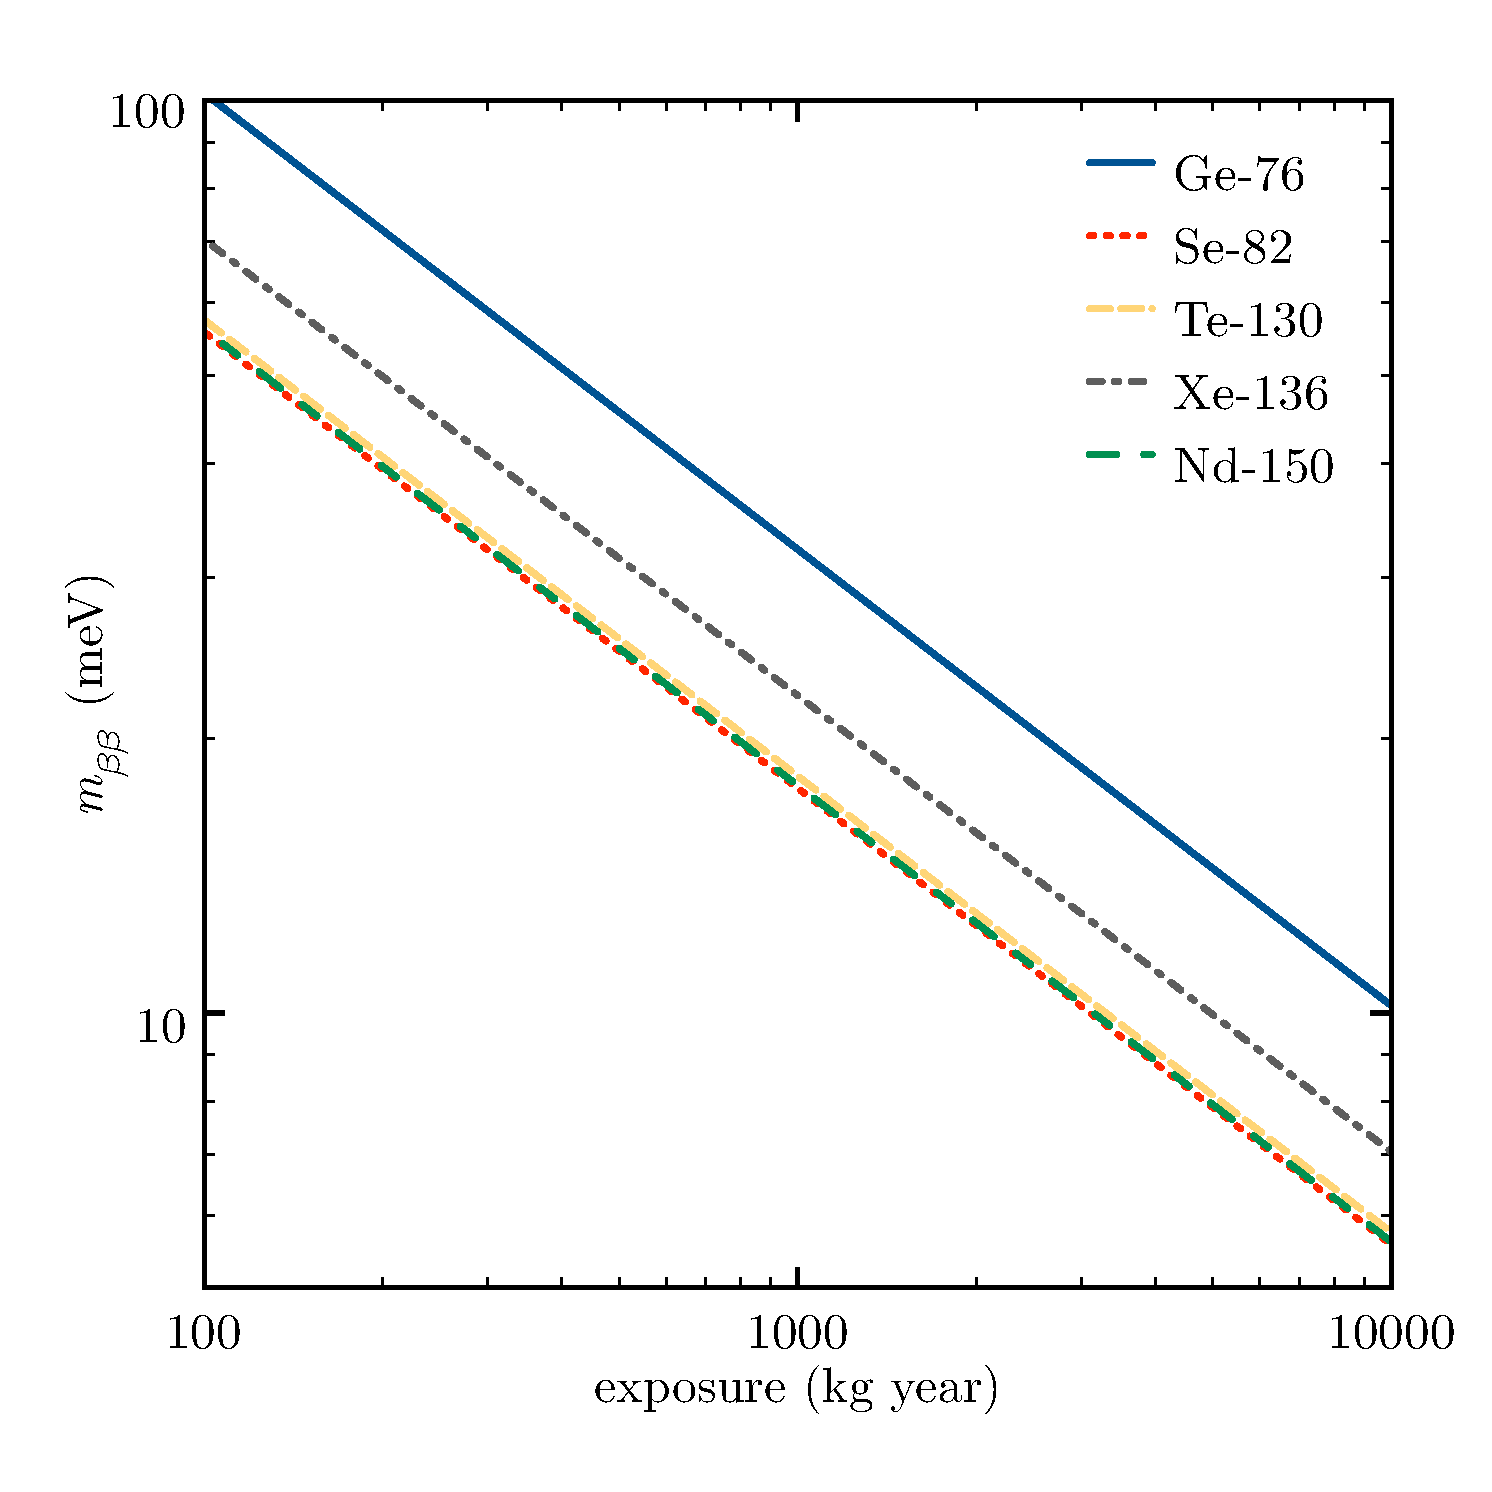
\includegraphics[width=0.65\textwidth]{img/isotopes_sensi.eps}
\end{center}
\caption{Sensitivity of ideal experiments at 90\% CL for different \bb\ isotopes. Since the yields are very similar, the sensitivities of \Se{82}, \Te{130} and \Nd{150} overlap. From reference \cite{Gomez-Cadenas:2010zcc}.} \label{fig:SensiIdeal}	
\end{figure}
%%%%%

%Condition iii) also requires choosing a \bb\ isotope with a high $Q_{\beta\beta}$ value. Backgrounds to \bbonu\ searches from natural radioactivity (see fig.~\ref{fig:decaychain}) populate the energy region below $\sim$3 MeV. This makes \Mo{100} which has a Q-value of 3034~keV, a very attractive candidate for \bbonu\ searches, and indeed it has been chosen as target by the future CUPID experiment. On the other hand, condition ii) requires an isotope with a \bbtnu\ mode as slow as possible. The best choice in this case would be \Xe{136} (the choice of EXO-200, kamLAND-Zen, NEXT, and the future nEXO experiment), which has a lifetime in excess of $10^21$~year. Instead, \Mo{100}\ has a lifetime two orders of magnitude faster ($\sim 10^21$~year), and would be disfavoured from this point of view. Conversely, experiments based in \Xe{136} have to deal with two important sources of background located very near the \Qbb\ of \Xe{136} ($\sim 2.5$ MeV), namely, 
%\Bi{214} (which emits a gamma that has a photoelectric peak at $\sim 2.4$ MeV), and \Tl{208} (which emits a gamma that has a photoelectric peak at $\sim 2.6$ MeV). The conclusion is that no ideal \bbonu\ isotope exists, and the choices of the different experiments imply alway a number of tradeoffs. 
%As the energy resolution degrades, the experiments are affected by \bbtnu\ backgrounds in a more or less pronounced way, depending on the isotope.  This is true unless the energy resolution of the experiment is truly excellent, in which case even relatively fast \bbtnu\ modes do not constitute a serious background to \bbonu\ searches. This is illustrated in fig.~\ref{fig:twonubgr}. In this figure, the \mbb\ sensitivity at 90\% CL is shown for ideal experiments using five different isotopes as a function of FWHM energy resolution. The experiments, each assumed to use 100 \kgbb\ of \bb\ emitter mass and to run for five years, are ideal in the sense of having perfect \bbonu\ efficiency and of being affected only by \bbtnu\ backgrounds. As fig.~\ref{fig:twonubgr} illustrates, and as far as the \bbtnu\ background is concerned and for the same moderate energy resolution (say, 5-10\% FWHM), \Xe{136} is to be preferred over \Se{82} and \Nd{150}, thanks to its much longer \bbtnu\ half-life (see tab.~\ref{tab:bb2nu_exp}). TODO: MENTION \Te{130} HERE. For experiments featuring excellent energy resolution, say $<2\%$ FWHM, all experiments would operate in a essentially \bbtnu\ background-free regime, for the assumed 500 \kgbb$\cdot$yr exposure. This is typically the case of \Ge{76}, \Mo{100} and some \Te{130} experiments, see sect.~\ref{subsec:energyresolution}.. In practice, however, other backgrounds are always present, typically creating a continuum through the region of interest, and a better resolution improves the experimental sensitivity even in the $<2\%$ FWHM energy resolution range.
%%%%%
%\begin{figure}[t!b!]
%\begin{center}
%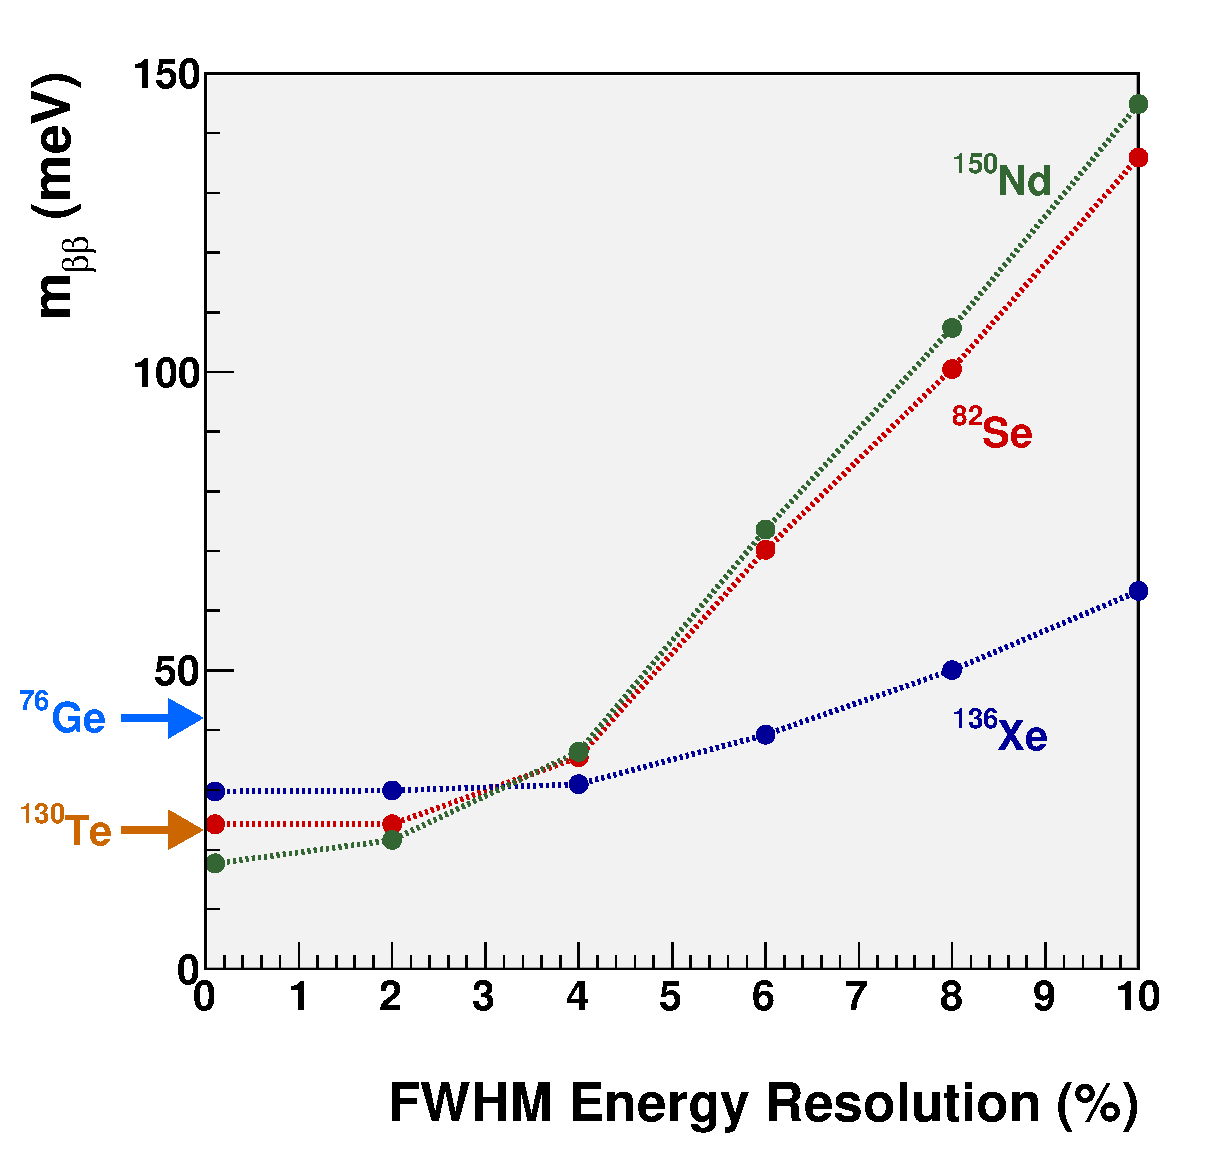
\includegraphics[width=0.65\textwidth]{img/mbbversusenergyres.eps}
%\end{center}
%\caption{\label{fig:twonubgr}Sensitivity to \mbb\ at 90\% CL as a function of FWHM energy resolution, for ideal experiments using five different isotopes, each with 100 \kgbb\ of \bb\ emitter mass and 5 years of data-taking. The experiments are assumed to have perfect efficiency and to be affected only by \bbtnu\ backgrounds. In practice, experiments using \Ge{76} and \Te{130} always feature an excellent energy resolution and are therefore not affected by \bbtnu\ backgrounds, hence only the background-free sensitivity limit is shown in those cases, with an arrow. TODO: REPEAT ADDING MO-100, AND REMOVING SE-82 AND ND-150? TE-130 SHOULD INCLUDE POOR RESOLUTION CASE, THINKING IN SNO+.}  
%\end{figure}
%%%%%

%Finally, another factor entering in the \bb\ isotope choice has to do with how well understood the nuclear physics for that isotope is. As we have seen in sect.~\ref{sec:nme}, the calculation of nuclear matrix elements is a very complicated task. In sect.~\ref{subsec:nme_current}, we have made an attempt at quantifying the uncertainties in the NMEs for various isotopes. Our conclusion is that no \emph{magic isotope} exists, and uncertainties in the 20--30\% range (according to our evaluation) exist for the five isotopes we have considered, \Ge{76}, \Se{82}, \Te{130}, \Xe{136} and \Nd{150}. TODO: UPDATE WITH UNCERTAINTIES FROM FOUR ISOTOPES ONLY: GE-76, MO-100, TE-130, XE-136.  


%%%%%%%%%%%%%%%%%%%%%%%%%%%%%%%%%%%%%%%%%%%%%%%%%%%%%%%%%%%%%%%%%%%%%%%%%%%
\subsubsection{Minimizing $\upsilon_2$: isotope mass}
%\subsection{Isotope mass} \label{subsec:isotope_mass}

%As explained above, large masses of \bb\ isotope are needed to explore the expected half-lives. 

One way to minimize $\upsilon_2$ is to maximize the mass of the isotope being deployed. This requires, in turn, candidates that are isotopically abundant (such as 
\Te{130} with a 34\%, isotopic abundance of the \bb\ emitter) and/or, easy to enrich and purify (such as \Xe{136})\footnote{The World production of both Xenon and Tellurium is also relatively high, in the range of few hundred tons/year.}.
%
%Consider \Xe{136} first. Xenon production is moderately high\footnote{The current xenon production is about 100 tons/yr, as a by-product of oxygen extraction from the air for the steel industry. Possible alternative techniques to increase this value are being explored \cite{Avasthi:2021lgy}.} and \Xe{136} is easier (and thus cheaper) to enrich that the other isotopes. The final product, a gas, is also easy to purify. \Te{136} is also attractive. Tellurium world production is even higher than that of xenon\footnote{estimated to be $\simeq$500 tons/yr} and has the advantage of having a high, 34\%, isotopic abundance of the \bb\ emitter, thus avoiding the   the need of isotopic enrichment, which greatly reduces costs. 
%
It is not surprising, therefore, that the large liquid-scintillator calorimeters have chosen those isotopes (KamLAND-Zen uses \Xe{136} and SNO+, \Te{130}), since both permit, with current technology, to deploy masses in the range of the ton (in fact the KamLAND-Zen experiment uses almost 800 kg of \Xe{136} already). Deploying even larger masses, in the range of 10 tons, appears feasible a priori. Xenon TPCs (the future nEXO and NEXT-HD experiments) will also use \Xe{136}, benefiting of the same advantages of the large calorimeters, e.g, the possibility of deploying large masses at relatively low cost, thanks to the economy of scale\footnote{The large liquid scintillator calorimeters, as well as the xenon TPCs, are all monolithic detectors, in which the volume, and therefore the mass, scales with the cubic power of the detector effective radius, while some ---but not all--- of the backgrounds scale with the detector surface, which is proportional to the radius squared.}. 

%Unfortunately, the \bb\ isotopes are not always abundant in nature, often requiring enrichment in order to obtain large, concentrated masses.

%The "economy of scale" of large monolithic detectors, such as isotope-loaded liquid scintillators or xenon TPCs, offers a clear advantage for amassing large quantities of \bb\ isotope. Modular approaches where many detector units (eg, crystals) share a common shielding/cryogenic infrastructure are a viable alternative. Let us now examine a few advantageous \bb\ isotopes, as far as mass is concerned.

%The current dedicated \bbonu\ experiment employing the largest amount of \bb\ isotope is a \Xe{136}-based one. The KamLAND-Zen 800 experiment uses xenon-loaded liquid scintillator contained in a spherical inner balloon. The amount of enriched xenon dissolved in the scintillator is 745~kg. Considering the (90.85$\pm$0.13)\% \Xe{136} isotopic abundance measured for the enriched xenon, this corresponds to 677~\kgbb\ of \Xe{136} \cite{KamLAND-Zen:2022tow}. There are two reasons that make \Xe{136} a popular choice for massive \bbonu\ experiments. First, its cost is relatively low, and world supply still sufficient for current \bbonu\ demands. The current xenon production is about 100 tons/yr, as a by-product of oxygen extraction from the air for the steel industry. Possible alternative techniques to increase this value are being explored \cite{Avasthi:2021lgy}. The second reason is that isotope enrichment for \Xe{136}, typically based on centrifuge separation methods, is relatively easy and, therefore, cheap. Starting from a 8.9\% isotopic abundance in natural xenon, $\simeq$90\% \Xe{136} isotopic enrichment is typical for \bbonu\ experiments. Beyond xenon-loaded scintillators, xenon TPCs (particularly cryogenic detectors with xenon in its compact, liquid, phase) also represent an excellent solution for large detectors. Dedicated \bbonu\ experiments typically use enriched xenon with $\simeq$90\% enrichment. Realistic proposals for such tonne-scale, or even multi-tonne-scale, experiments exist (see sect.~\ref{subsec:XeTPCs}). Very massive and low-background TPCs filled with natural xenon, primarily developed for direct dark matter searches, also allow for potentially sensitive \bbonu\ searches. One example is the onngoing LUX-ZEPLIN (LZ) experiment, containing about 500~\kgbb\ of \Xe{136} within its 5.6 ton fiducial volume \cite{LZ:2019qdm}.

%Liquid scintillator proposals permit in principle to reach large \bbonu\ isotope masses with other isotopes as well, particularly \Te{130}. Tellurium world production is estimated to be $\simeq$500 tons/yr. Tellurium has the advantage of having a high, 34\%, isotopic abundance of the \bb\ emitter \Te{130}. Therefore, the need of isotopic enrichment is typically not considered for \Te{130}-based experiments, greatly reducing costs. Methods for loading \Te{130} into organic liquid scintillators have been developed, particularly in the context of the SNO+ Collaboration. Loading levels up to $\mathcal{O}$(1\%) \Te{130} by weight may be possible in large detetors. Light levels were measured to be reduced compared to unloaded scintillators, but still acceptable. Stability of the loading has been demonstrated on the timescale of years. Water-based liquid scintillators may also be loaded with similar percentages of \Te{130}. Thus, several tons of \Te{130} may be loaded in large liquid scintillator detectors.

%High-resolution crystals, that is germanium diodes and bolometers, are compact and modular detectors. They might also be scalable to large masses. The raw \bb\ materials used in this case are available in large supplies, and do not constitute a practical limitation toward massive \bbonu\ experiments. A more challenging scalability aspect is the crystal growth process necessary to fabricate large, kg-scale, crystals of high purity.   

%The LEGEND-200 experiment has started taking physics data in 2023. With about 100 high-purity germanium detectors of 0.5--4~kg mass and 86--91\% \Ge{76} enrichment each, a total of about 170~\kgbb\ of \Ge{76} is used. LEGEND-200 has deployed the enriched detectors from the previous GERDA and the Majorana Demonstrator experiments, together with newly-produced inverted-coaxial point-contact (ICPC) detectors, in an upgraded GERDA infrastructure at LNGS. A second phase with 5 times more \Ge{76} mass, LEGEND-1000, is being planned.

%The CUORE experiment is searching for the \bbonu\ of \Te{130} with an array of 988 bolometers since 2017. Each bolometer consists of a 750~g $^{nat}$TeO$_2$ crystal, for a total TeO$_2$ mass of over 742 kg, which corresponds to 206~\kgbb\ of \Te{130} \cite{CUORE:2021mvw}. Beyond scalability, bolometers also offer isotopic flexibility. The CUPID-Mo demonstrator \cite{Augier:2022znx} searched for \Mo{100} \bbonu\ with twenty enriched Li$_2$$^{100}$MoO$_4$ (LMO) scintillating calorimeters, each with a mass of about 210~g. Considering the $\simeq$97\% \Mo{100} enrichment, about 2.3~\kgbb\ of \Mo{100} was employed in CUPID-Mo. CUPID is a proposed successor experiment of CUORE based on the CUPID-Mo technology, which plans to use about 250~\kgbb\ of \Mo{100} \cite{CUPID:2019imh}.


%%%%%%%%%%%%%%%%%%%%%%%%%%%%%%%%%%%%%%%%%%%%%%%%%%%%%%%%%%%%%%%%%%%%%%%%%%%

\subsubsection{Minimizing $\upsilon_2$: Energy resolution} %\label{subsec:energyresolution}
%
%Together with a large isotope mass, good energy resolution is a necessary (but not sufficient!) requirement for the \emph{ultimate} \bbonu\ experiment. It is the only protection against the intrinsic \bbtnu\ background, and improves the signal-to-noise ratio in the region of interest around \Qbb. 

Why then, choose \Ge{76} (LEGEND) or \Mo{100} (CUPID) for future \bbonu\ experiments, given the fact that the raw material will be more difficult to enrich and purify (thus more expensive, and presumably harder to produce in large quantities)? %Furthermore, both experiments will be based in piling up individual crystals, benefitting less of economy of scale than large liquid scintillators calorimeters (LLSC) and xenon TPCs (XeTPCs)
%
The answer to this question is energy resolution. The resolution of both KamLAND-Zen and SNO+, is of the order of 10\%\footnote{Unless otherwise stated all resolutions in this review are FWHM.} dominated by fluctuations in the light collection of their PMTs. EXO measured a resolution of about 3 \%, and nEXO expects $\simeq$2 \%, while NEXT-White has measured 1\% and NEXT-100, as well as NEXT-HD, expects to improve that number to 0.5-0.7 \%. Instead, 
GERDA measured a spectacular resolution of 0.16\% (3.3$\pm$0.4~keV at 2039~keV\cite{GERDA:2020xhi}) and the crystals constituting the bulk of the LEGEND-200 experiment feature an even better energy resolution of 0.14\% (2.9$\pm$0.1~keV)  (FWHM). CUPID, on the other side, will deploy crystals of 
lithium molybdate (LMO, Li$_2$$^{100}$MoO$_4$), for which the measured resolution is 0.25\% ($7.6 \pm 0.7$ keV at  3034~keV \cite{CUPID:2020aow}). In both cases, therefore, the experiments have prioritized energy resolution over mass. Notice that both factors compensate each other in $\upsilon_2$. 

%The detectors for \bb\ searches that have achieved the best energy resolution so far are the \emph{germanium diodes} and the \emph{bolometers}. 

%In germanium detectors the energy is measured via ionization (creation of electron-hole pairs in the semiconductor). The exposure-averaged FWHM energy resolution of the Ge detectors used in the final GERDA Phase II result was only 3.3$\pm$0.4~keV \cite{GERDA:2020xhi}. Considering that the \Qbb\ value in \Ge{76} is 2039~keV, this corresponds to a relative energy resolution of 0.16\% (FWHM). In particular, the large ICPC-type detectors constituting the bulk of the LEGEND-200 detectors featured an even better energy resolution of 2.9$\pm$0.1~keV (FWHM). 

%In bolometers the energy is measured by detecting a temperature rise in crystals with very small specific heat. Several bolometric crystals have been proposed and tested for \bb\ searches, such as tellurite (TeO$_{2}$), lithium molybdate (LMO, Li$_2$$^{100}$MoO$_4$) and zinc selenide (ZnSe). For these three technologies, FWHM energy resolutions at the Q-values of the corresponding \bb\ emitters were measured to be: 7.8$\pm$0.5 \cite{CUORE:2021mvw}, 7.6$\pm$0.7 \cite{CUPID:2020aow} and 21.8$\pm$0.3 keV \cite{CUPID:2022puj}, respectively. TeO$_{2}$ and LMO detectors thus feature similar resolution performance among them based on the heat measurement, and superior to the ZnSe one. However, as we will see in the following (sect.~\ref{subsec:bgr_mitigation}), LMO detectors offer an advantage over TeO$_{2}$ ones, as they provide an additional scintillation light signal.



 
%%%%%%%%%%%%%%%%%%%%%%%%%%%%%%%%%%%%%%%%%%%%%%%%%%%%%%%%%%%%%%%%%%%%%%%%%%

\subsubsection{Minimizing $\upsilon_2$: Background index} %\label{subsec:bgr_mitigation}

Minimizing the background index, $c$, in $\upsilon_2$, is the main business of 
\bbonu\ experiments. In addition to passive techniques, discussed in 
\ref{subsec:bgrmitigation}, active techniques, which involve detector information, are used to achieve the lowest possible background rate.

%Double beta decay experiments are mostly about suppressing the background sources mentioned in Sect.~\ref{subsec:bgr_sources}. As we have seen already, the mere presence of background in the region of interest around \Qbb\ changes the regime of the \mbb\ sensitivity from a $(\Mbb \cdot t)^{-1/2}$ dependence to $(\Mbb \cdot t)^{-1/4}$. In the following, we describe the 
%Background mitigation techniques can be separated into {\emph passive} and {\emph active}, depending on whether detector information is used or not.

External to the detectors themselves, experiment make extensive use of {active} veto systems, such as 
liquid shields in the form of water tanks, LAr-filled cryostats or liquid scintillator buffers. Such shields are instrumented with Cherenkov/scintillation light detectors in order to tag the passage of charged particles. Plastic scintillator detectors are also often used as active veto systems against external backgrounds. Such anti-coincidence techniques, between an inner detector containing the \bbonu\ target and outer detectors, constitute a powerful active background mitigation technique. 

%Excellent energy resolution is, of course, another powerful active background mitigation technique, as already discussed. There are, however, many other active background mitigation techniques beyond veto systems and energy resolution. 

In addition to anti-coincidence requirements in space, delayed coincidences in time are also used to suppress backgrounds. This is the case for sequential radioactive decays with relatively short-lived isotopes. A prime example is \Bi{214}-induced background suppression via the delayed \Po{214} tag, where the \Po{214} $\alpha$ decay has a 164.3~$\mu$s half-life. 

Signal and background events have also different spatial distributions. Signal events are typically distributed uniformly in the detector volume. External backgrounds accumulate on, or enter from, detector surfaces. This is also exploited to suppress backgrounds via detector fiducialization. 

The topological information of the energy deposits in the active volume is also used. Gamma-ray background interactions producing multi-site energy deposits, typically via multi-Compton interactions, may be readily vetoed in segmented or imaging detectors. Pulse shape analysis in individual Ge detectors is an alternative way to identify and suppress multi-site backgrounds. Low density detectors, such as xenon gas TPCs where MeV-scale particles produce extended tracks, provide even more detailed topological information. In this case, information from the reconstructed $dE/dx$ energy loss profiles along the track can distinguish single-electron background events from double-electron signal events.

Particle identification is another powerful background suppression handle. A notable example is $\alpha/\beta$ discrimination in scintillating bolometers. As the light yield for energy depositions induced by $\alpha$ and $\beta$ particles of the same energy is different, the simultaneous detection of light and heat leads to an effective rejection of the $\alpha$ background. 

Finally, a powerful handle, used by both liquid scintillator detectors (KamLAND-Zen, SNO+) and LXe TPCs (nEXO) is {\em self-shielding}. 

%Finally, another handle to suppress non-\bbtnu\ backgrounds is \emph{daughter ion tagging} in coincidence with the detection of the two beta electrons. This has been proposed, and is actively being pursued, for both liquid and gas xenon TPC detectors. In this case, the \bbonu\ decay is ${\rm ^{136}Xe}\to {\rm ^{136}Ba^{++}}+2e^-$. In liquid, the \Ba{136}$^{++}$ ion rapidly captures an electron in the charge cloud following a \bb\ event, resulting in \Ba{136}$^{+}$, and barium neutralization may also occur. In the less dense gas environment, no recombination is expected, and the \Ba{136}$^{++}$ doubly-charged state remains stable. Recently, both the nEXO \cite{nEXO:2018nxx} and NEXT \cite{McDonald:2017izm,Rivilla:2020cvm} collaborations made substantial progress in isolating and detecting a lone Ba ion in-situ, via fluorescence imaging techniques. Daughter ion tagging is undoubtedly very challenging from the technical point of view, but the payoff would be huge if the R\&D were to be successful.

The lowest background indeces ($c$ term in eq.~\ref{eq:mbbx2}, expressed in terms of background events per unit energy, \bb\ isotope mass and exposure time) in a \bbonu\ experiment so far were achieved by the KamLAND-Zen (see sect.~\ref{subsec:liquid_scint}) and GERDA (sect.~\ref{subsec:hpge}) experiments. Perhaps not surprisingly, given the importance of background suppression in \bbonu\ experiments, these are also the two experiments with the most stringent \bbonu\ half-life upper limits to date. KamLAND-Zen  has achieved a background index of $1.3\times 10^{-4}$ \ckkbby\ \cite{KamLAND-Zen:2022tow}, thanks to its outstanding radio-purity, self-shielding and anti-coincidence techniques. On the other hand, GERDA Phase II has achieved $6.0\times 10^{-4}$ \ckkbby\ \cite{GERDA:2020xhi}, thanks to its ultra-pure crystals and pulse shape discrimination techniques. 

It is interesting to compare $\upsilon_2$ for both experiments. In the case of KamLAND-Zen, $\Mbb\cdot t = 970$ \kgbb$\cdot$year, while for GERDA 
$\Mbb\cdot t \sim 127$ \kgbb$\cdot$year. Thus, the product $c/(\Mbb\cdot t)$ yields a factor of 
$(6/1.3) \cdot (970/127) = 35$ in favor of KamLAND-Zen, which is more than compensated with the ratio of resolutions $10/0.16 = 62.5$. Indeed, in spite of its relatively modest exposure, GERDA combines an excellent background index and superb resolution to obtain the best value of the figure of merit $\upsilon_2$. 
%On the other hand, KamLAND-Zen compensates the difference with better $\upsilon_1$ (e.g, better phase space factor) and both experiment obtain similar sensitivity to the \bbonu\ decay lifetime, 

%Finally, we remark that the relevant background figure of merit, the one appearing in the \mbb\ sensitivity of eq.~\ref{eq:mbbx3}, is given by the product $c\cdot \Delta E$, that is the number of background events per unit time and \bb\ isotope mass in the entire region of interest\footnote{For simplicity, we are assuming here that the energy regiopn of interest around \Qbb\ has a width equal to the FWHM energy resolution, $\Delta E$.}. According to this figure of merit, GERDA Phase II is the current record holder in terms of lowest background conditions, with a $c\cdot \Delta E$ value of 0.002 counts/$(\kgbb\cdot\ensuremath{year})$. Considering that GERDA Phase II has accumulated a total exposure of 90.2 \kgbb$\cdot$year, the mean number of background events expected within \Qbb $\pm$ FWHM/2 was about 0.2, consistent with observations. In other words, GERDA Phase II accomplished its goal of background-free conditions. The goal of the new-generation experiments is typically to reach $10^{-4}$ \ckkbby\ background levels, and sometimes significantly better than that (eg, LEGEND-1000).



%%%%%%%%%%%%%%%%%%%%%%%%%%%%%%%%%%%%%%%%%%%%%%%%%%%%%%%%%%%%%%%%%%%%%%%%%%

\subsubsection{Detection efficiency} 
%\label{subsec:efficiency}

Minimizing \mbb\ requires, according to eq.~(\ref{eq:mbbx3}), maximizing the detector efficiency $\epsilon$. Notice that, when compared with the terms in $\upsilon_2$, 
the efficiency enters as $\epsilon^2$. 
%Neutrinoless double beta decay events are extremely rare, if present at all, thus a high detection efficiency is an important requirement for a \bb\ experiment. Equation~(\ref{eq:mbbx3}) clearly indicates that the detector design should prioritize a high detection efficiency. 
To obtain the same increase in \mbb\ sensitivity obtained by doubling the efficiency, the mass would have to be increased by a factor of 4, or the factor
$c\cdot \Delta E$ decreased by a factor of 4. 

In general, the simpler the detection scheme, the higher the detection efficiency. Homogeneous detectors, 
%where the source material is the detection medium, provide in principle higher efficiency than a separate-source approach. This is due to a number of reasons, including geometric acceptance, absorption in the \bb\ source, back-scattering of electrons, and tracking requirements.
and in particular 
pure calorimetric approaches such as germanium diodes or bolometers, tend to have the highest total signal efficiencies, and values in excess of 75\% have been obtained. 
%
%For the CUORE bolometric \bbonu\ search in \Te{130}, the total efficiency is 81.6$\pm$0.2\%, given by the product of the reconstruction, anti-coincidence, pulse shape discrimination and containment efficiencies \cite{CUORE:2021mvw}. The main inefficiency comes from containment requirements, accounting for the energy loss due to geometrical effects as well as bremsstrahlung.

%In the case of germanium diodes, the exposure-averaged efficiency in the final GERDA \bbonu\ search was 63.0$\pm$5.6\%, given by the product of electron containment, active volume, liquid argon veto and pulse shape discrimination requirements \cite{GERDA:2020xhi}. For the ICPC-type detectors alone employed in LEGEND-200, the total efficiency increases to 75.2$\pm$2.1\%, thanks to their larger crystal sizes and intrinsically better performance.
%
Large liquid scintillators may also have relatively high efficiencies. This is especially the case when the \bb\ source is enclosed in a inner balloon surrounded by a scintillator buffer region, as in the KamLAND-Zen experiment. Also,
%The detector dead-time to tag and reject comsogenic backgrounds (about $\simeq$15\% in \cite{KamLAND-Zen:2022tow}) is a relevant inefficiency, in this case. Depending on the \bbonu\ analysis details, the relatively poor energy and spatial resolutions may also introduce, effectively, additional inefficiencies. For example, about 22\% of the putative \bbonu\ events would fall outside a 350~keV wide energy region of interest around \Qbb\ in \cite{KamLAND-Zen:2022tow}.
%
Liquid xenon TPCs share the same advantages of the other dense, homogeneous, detectors. However, both the large liquid scintillator calorimeters and the LXe TPCs, use a large fraction of their active mass as self-shielding. This implies, either giving away a substantial fraction of the mass (for example performing the analysis in a reduced volume close to the center of the detector in KamLAND-Zen, SNO+ or nEXO), or weighting the events in the outer shells of the detector to take into account the increased background. In both cases, one has to be careful with the definition of efficiency. Self-shielding does not come for free.  
%they use some of the \bb\ mass close to the detector borders effectively for self-shielding, paying it with some efficiency loss.

Unlike LXeTPCs, HPXeTPCs such as those being developed by NEXT do not rely on self-shielding for background reduction, but use instead particle tracking, which also comes at the expenses of a significant efficiency loss.
%Some experiments perform particle tracking, such as planar configurations of \bb\ foils separate from detector media, or homogeneous xenon gas TPC. The tracking requirements typically cause a significant efficiency loss. 


%%%%%%%%%%%%%%%%%%%%%%%%%%%%%%%%%%%%%%%%%%%%%%%%%%%%%%%%%%%%%%%%%%%%%%%%%

\section{The past, present and future of neutrinoless double beta decay experiments} \label{sec:experiments}
%%%
The search for double beta decay has a long history, approaching now a full century. Initially, and for decades, the field was dominated by geochemical measurements (e.g., \cite{Inghram:1950qv}), which looked for evidence of \bb-decay products in geologically old ($\sim 10^9$ years) minerals rich in the parent isotope. An excess of the daughter isotope over its natural concentration was interpreted as evidence for \bb\ decay (either \bbtnu\ or \bbonu, as the method cannot distinguish between them). 

It was not until 1987 that the \bbtnu\ decay mode was directly observed in the laboratory \cite{Elliott:1987kp,Moe:2014ioa}. The detector employed was a fairly large ($\sim1$ m$^{3}$) time projection chamber with a \bb\ source (14~g of enriched \Se{82}) deposited on a thin foil that formed the central electrode of the chamber. The trajectories of the electrons emitted from the source foil were recorded by the TPC and then analyzed to infer their energy and kinematic features. Since this initial detection, the two-neutrino mode has been directly observed for eight other isotopes in several experiments (see table~\ref{tab:bb2nu_exp} for further details).

By contrast, no evidence of \bbonu\ decay has been found so far. Nevertheless, the progress made in the last two decades in the development of ultra-low-background detection technologies has been extraordinary. The experimental goal for the next generation of experiments is the exploration of the region of half-lives, first up to $10^{27}$~years and eventually up to $10^{28}$~year. This will, ultimately, require exposures well beyond 1~ton~year and background rates lower than 1~count~ton$^{-1}$~yr$^{-1}$. 
%Only a few of the experimental techniques presently considered will be able to attain those levels. Besides, given the scale and cost of future experiments, the consolidation of the international effort will be essential.

In this section, we review the most promising technologies for the next generation of experiments, summarizing the results of past experiments, their current status and future plans. This discussion does not pretend to be exhaustive; the reader is referred to the cited publications for more details.

\subsection{High-purity germanium detectors} 
\label{subsec:hpge}
%
Germanium can be enriched in the \bb\ isotope \Ge{76}and transformed into high-purity germanium (HPGe) detectors, devices characterized by superb energy resolution and high efficiency. 

HPGe detectors have a long-standing record in neutrinoless double beta decay searches, going back to the late 1960s \cite{Fiorini:1967in,Fiorini:1970}. In the 1990s, the two most sensitive experiments used this technology: \textsc{Heidelberg-Moscow} (HM) ran in the Laboratori Nazionali del Gran Sasso (LNGS) and set a lower limit on the \bbonu\ half-life of \Ge{76} of $1.9 \times 10^{25}$~years (90\% CL) \cite{Klapdor-Kleingrothaus:2000eir}; the International Germanium Experiment (IGEX) operated in the Homestake Mine (USA), Canfranc (Spain) and the Baksan Neutrino Observatory (Russia), setting a slightly worse limit than HM, $T^{0\nu}_{1/2}(\Ge{76}) \geq 1.6 \times 10^{25}$~years (90\% CL) \cite{IGEX:2002bce}. A subset of the HM collaboration published a controversial claim of evidence for \bbonu\ decay \cite{Klapdor-Kleingrothaus:2001oba, Klapdor-Kleingrothaus:2006zcr}, which sparked at the time an intense debate in the community (see, for example, ref.~\cite{Aalseth:2002dt}). 

HM and IGEX were succeeded by two new experiments, the GERmanium Detector Array (GERDA) \cite{GERDA:2020xhi} and the \textsc{Majorana Demonstrator} \cite{Majorana:2022udl}, which employed novel types of HPGe devices with improved energy resolution and pulse-shape identification (i.e., detailed information about the topology of events through the time structure of the recorded charge signal). GERDA, located at LNGS, operated bare HPGe detectors in a high-purity instrumented liquid argon (LAr) cryostat, which provided not only the cooling for the HPGe devices, but also served as active shielding and veto against external and internal background events. With a background index of $5.2\times10^{-4}$~\ckky\ and an energy resolution of $\sim3$~keV (FWHM) at $Q_{\bb}=2039$~keV \cite{GERDA:2020xhi}, GERDA has been the first \bbonu-decay experiment to operate in virtually background-free conditions (i.e., less than one background count in the signal window). With a total published exposure of 127.2~kg~yr, the derived lower limit on the \bbonu\ half-life of \Ge{76} is $1.8\times10^{26}$~yr (90\% C.L.) \cite{GERDA:2020xhi}. The \textsc{Majorana Demonstrator} operated its HPGe detectors at the Sanford Underground Research Facility (SURF) in a high-purity shield built with electro-formed copper produced deep underground. With a world-leading energy resolution of 2.52~keV FWHM at the $Q$ value and after accumulating an exposure of 64.5~kg~yr, the experiment set a half-life lower limit of $8.3\times10^{25}$~yr (90\% CL) \cite{Majorana:2022udl}.

Building on the success of GERDA and the \textsc{Majorana Demonstrator}, the LEGEND \cite{LEGEND:2021bnm} collaboration is developing a staged \bbonu-decay experimental program aiming at an ultimate sensitivity to the \Ge{76} half-life beyond $10^{28}$~years. 
LEGEND will make use of new inverted-coaxial point-contact (ICPC) HPGe detectors with exceptional energy resolution (0.12\% FWHM at 2039~keV) and more than a factor of two greater mass per crystal over previous experiments. As done in GERDA, the HPGe detectors will be operated immersed in LAr.

%%%%%
\begin{figure}[t!b!]
\begin{center}
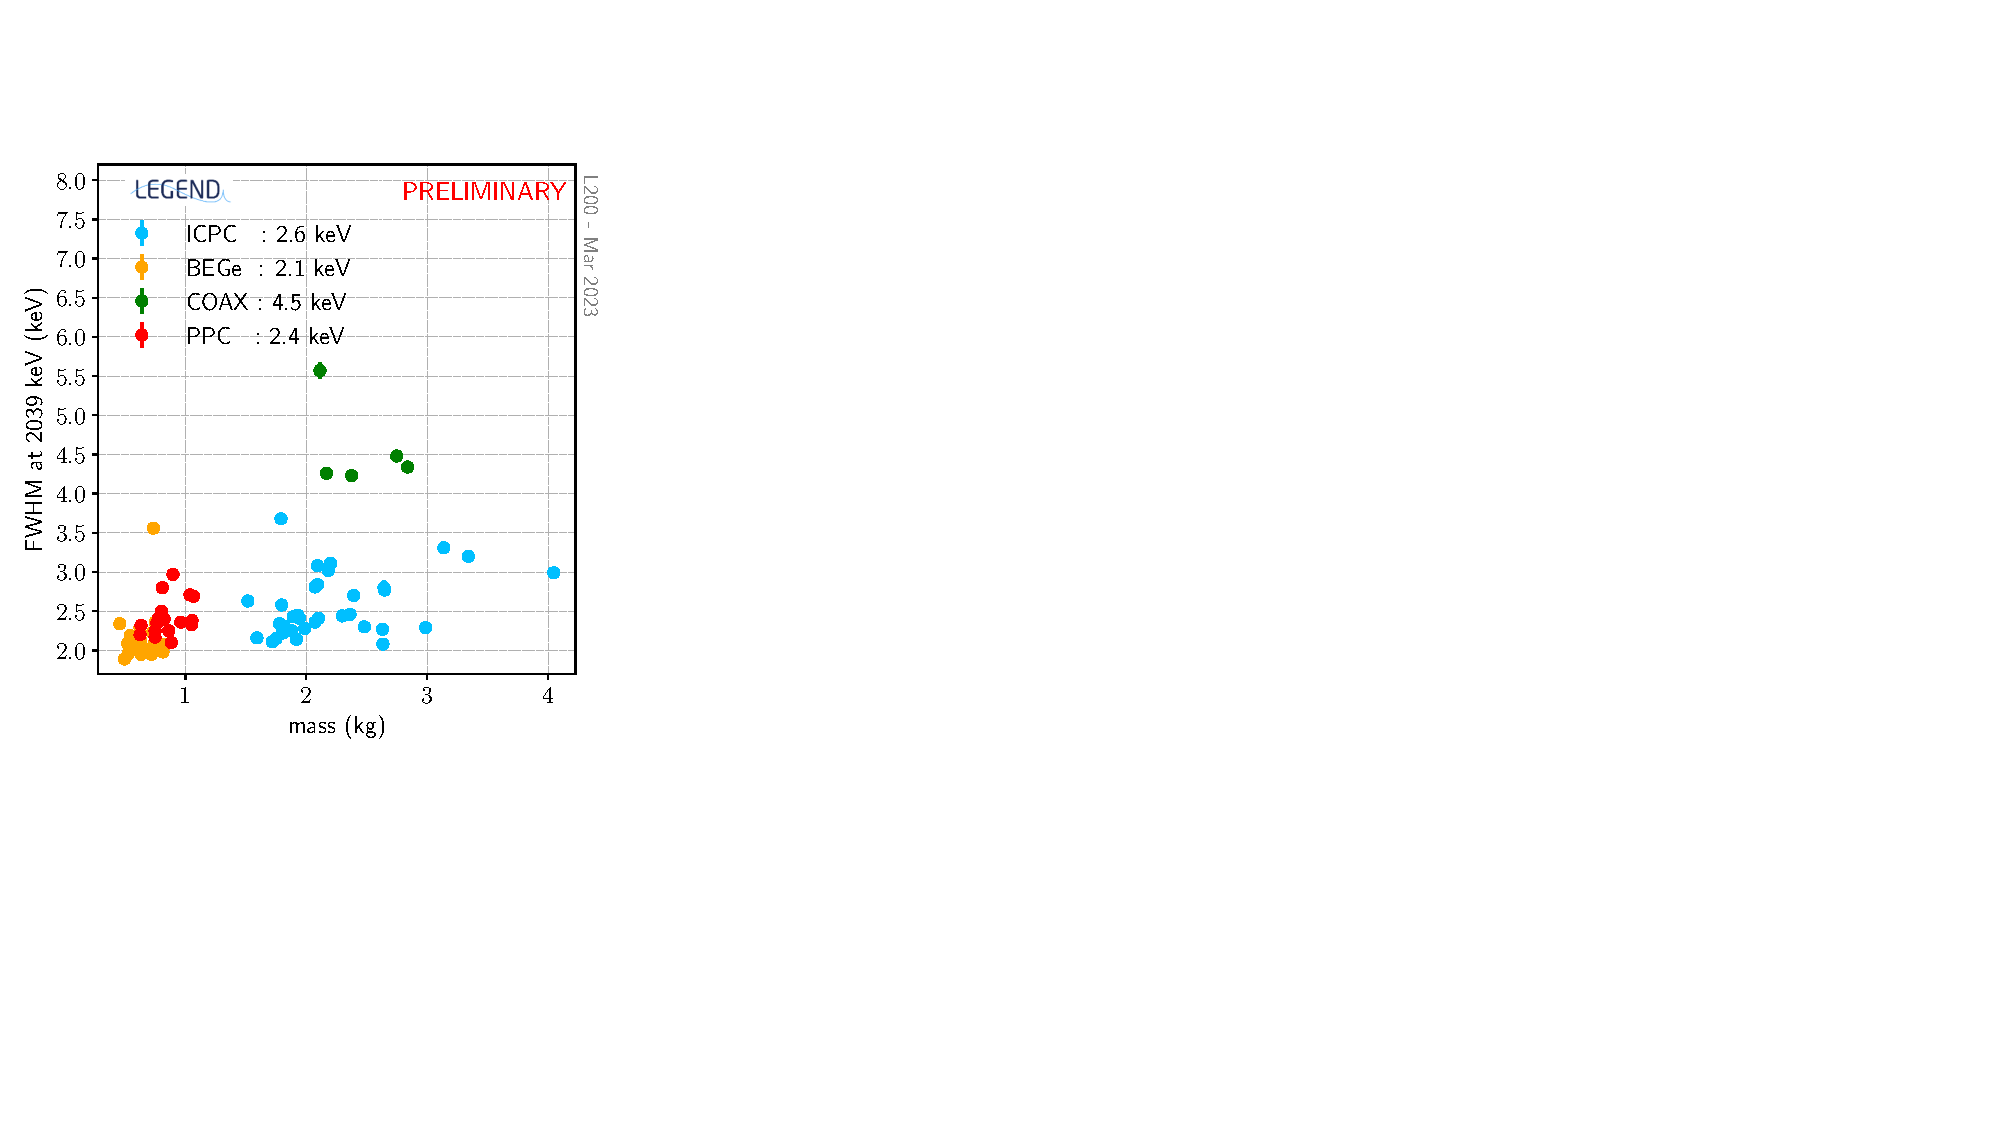
\includegraphics[width=0.55\textwidth]{img/legend-200.pdf}
\end{center}
\caption{Preliminary FWHM energy resolution at the \Ge{76} Q-value for the $\sim$100 HPGe detectors currently deployed in LEGEND-200. The different colors indicate different HPGe detector types.}  \label{fig:legend-200}
\end{figure}
%%%%%

LEGEND-200, the first phase of the experiment, is operating 200~kg of germanium detectors ---\thinspace the existing 70 kg of enriched detectors from the \textsc{Majorana Demonstrator} and GERDA, plus an additional 130~kg of newly produced ICPC detectors\thinspace--- in an upgrade of the GERDA infrastructures at LNGS incorporating technologies from the \textsc{Majorana Demonstrator}. First LEGEND-200 results related to its outstanding energy resolution are shown in Fig.~\ref{fig:legend-200}. A reduction by a factor of 2.5 with respect to the GERDA background rate is expected, aiming at a sensitivity to the \bbonu\ half-life of about $10^{27}$~yr for  an exposure of 1 ton~yr. The second phase of the experiment, LEGEND-1000, has a background goal of less than $10^{-5}$~\ckky, a 20-fold reduction with respect to LEGEND-200 expected to come from the use of underground-sourced argon (which does not contain the radioactive isotopes $^{42}$Ar and its daughter $^{42}$K), improvements in the radiopurity of materials and the exclusive use of ICPC HPGe detectors.


\subsection{Bolometers} \label{subsec:bolometers}
%
A bolometer for \bbonu-decay searches consists of a dielectric crystal, which contains the isotope of interest, coupled to a temperature sensor. When the bolometer is cooled to very low temperatures ($<20$~mK for crystals with masses in the 0.1--1~kg range), the energy deposited in the crystal by interacting particles can be measured with high precision as a rise in temperature. This technique, originally proposed for rare-event searches in the early 1980s \cite{Fiorini:1983yj}, can provide an energy resolution at the few per-mil level (FWHM) at 3~MeV and a total efficiency at the 70\%--90\% level. Bolometer-based detectors ---\thinspace at very different scales and maturity levels \thinspace--- have been used to search for \bbonu\ in six different nuclides ($^{48}$Ca, $^{82}$Se, $^{100}Mo$, $^{116}$Cd, $^{124}$Sn and $^{130}$Te) since the 1990s.

The MiDBD experiment \cite{Arnaboldi:2002te} at LNGS was the first bolometric array with large-mass crystals. It consisted of 20 TeO$_2$ bolometers of 340~g each ($3\times3\times6$~cm$^3$ crystals). MiDBD proved that an energy resolution of 5~keV at the $Q$ value was within reach, and achieved a background rate of less than 1~\ckky\ in the region of interest around \Qbb. With a total exposure of 4.25~kg~yr, MiDBD set the limit $T_{1/2}^{0\nu}(\Te{130}) > 2.1\times10^{23}$~years at 90\% CL. 

CUORICINO \cite{Andreotti:2010vj}, an array of 62 TeO$_2$ crystals, improved on the MiDBD results after running between 2003 and 2008 at LNGS, accumulating a total exposure of 19.75~kg~yr. It set a lower bound on the \Te{130} half-life of $2.8\times10^{24}$~years at 90\% CL. 

The latest step in this long series of TeO$_2$ bolometric detectors is CUORE \cite{CUORE:2021mvw}, currently taking data at LNGS and consisting of 988 bolometers with a mass of about 750~g each, corresponding to about 200 kg of \Te{130}. So far, the experiment has set a lower limit of $2.2\times10^{25}$~years on the half-life of \Te{130} for an exposure of 288.8~kg~yr. The background rate, $(1.49\pm0.04)\times 10^{-2}$~\ckky, is dominated by energy-degraded $\alpha$ particles generated by surface contamination. CUORE will continue to take data until it reaches its design \Te{130} exposure of 1~ton~yr. 

Scintillating bolometers could bring an additional handle for the discrimination between signal and background \cite{Pirro:2005ar}. In these devices, the crystal containing the isotope of interest is a scintillator, and a second auxiliary bolometer is operated close to it to register the emitted scintillation light. The simultaneous detection of heat and scintillation allows one to distinguish $\alpha$ particles from electrons or $\gamma$ rays thanks to their different light yield and signal shape, eliminating the dominant background source observed in CUORE. This and other background reduction techniques are the subject of an intense, world-wide R\&D program; for more details, see, for example, \cite{Zolotarova:2021inw} and references therein.

%%%%%
\begin{figure}[t!b!]
\begin{center}
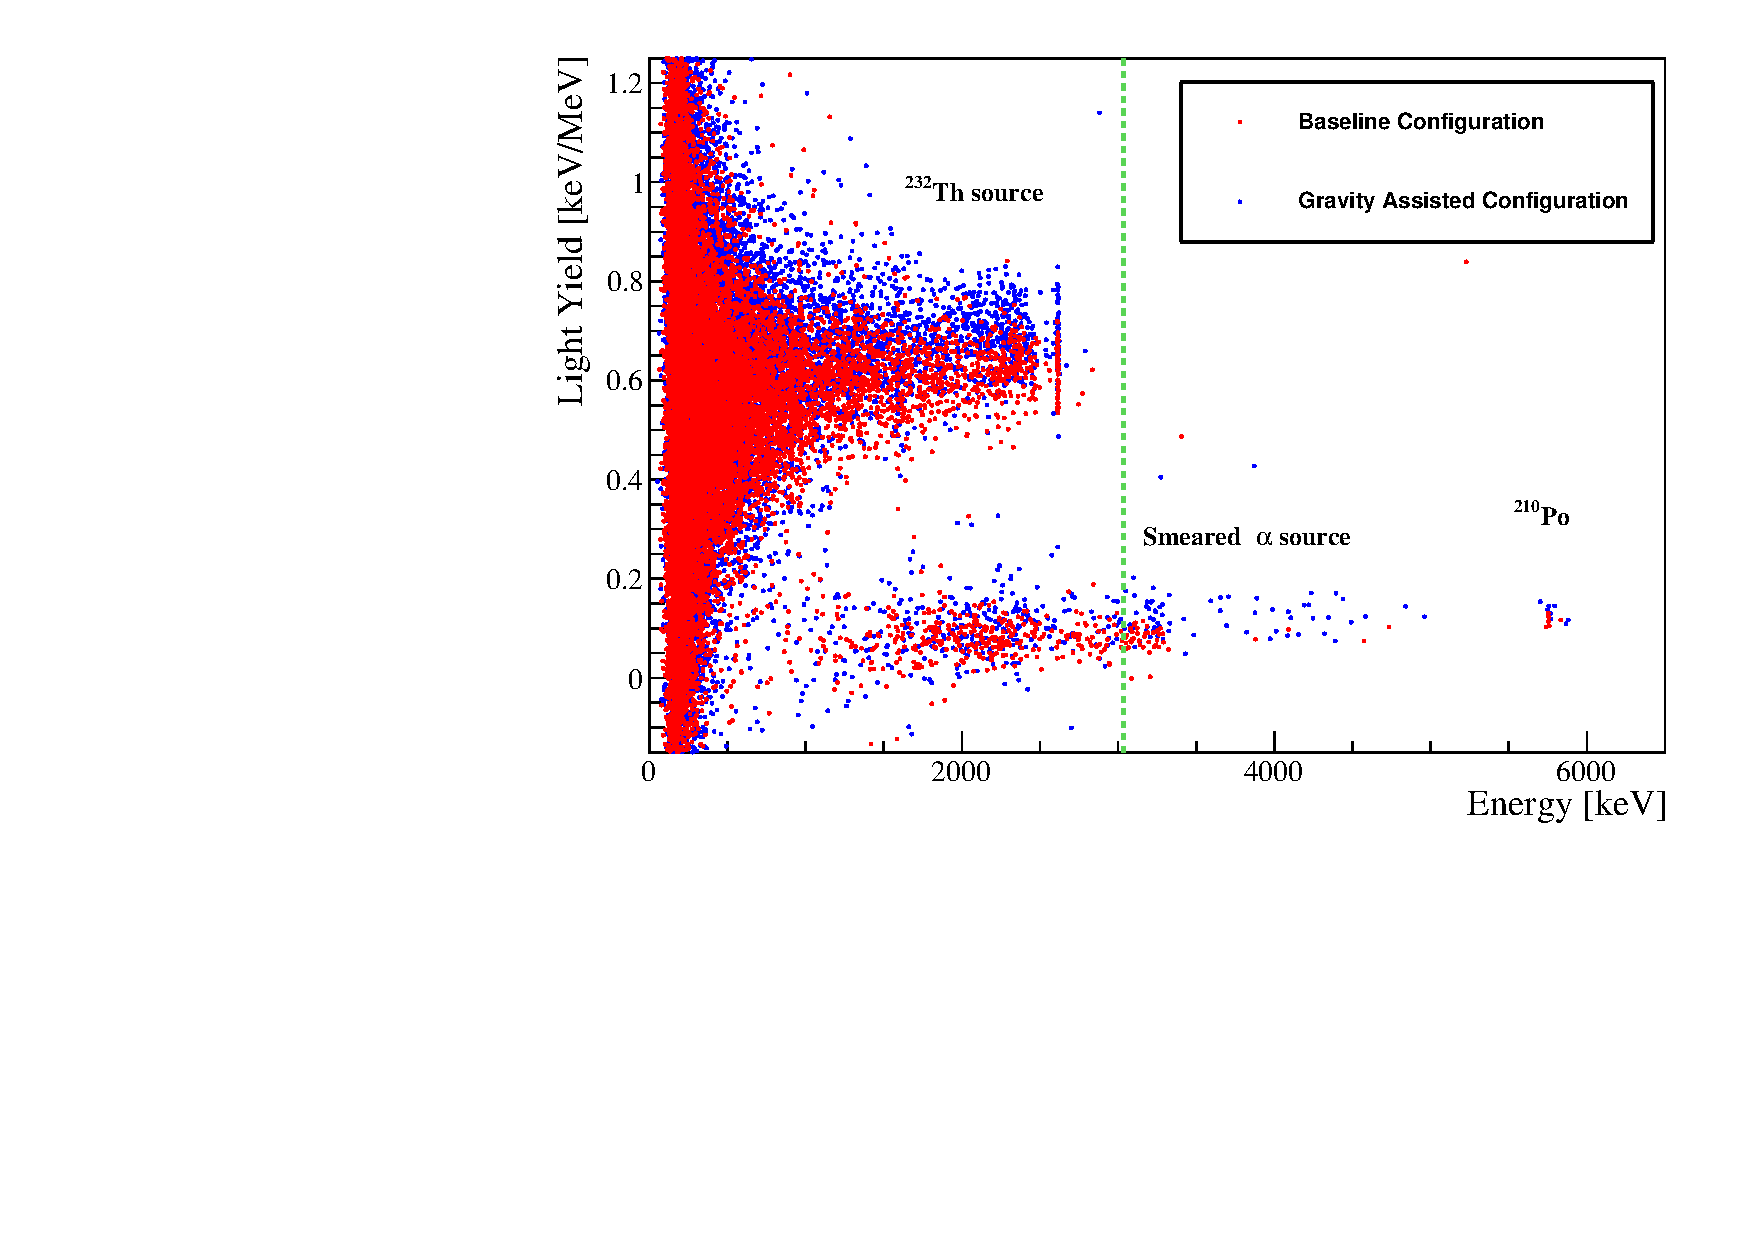
\includegraphics[width=0.8\textwidth]{img/cupid.pdf}
\end{center}
\caption{Light yield per unit energy as a function of the energy deposited in the LMO crystal, for two different configurations under study as part of the CUPID detector optimization process. The green vertical line indicates the Q-value of \Mo{100}. Taken from \cite{CUPID:2022opf}.} \label{fig:cupid}
\end{figure}
%%%%%

The CUPID (CUORE Upgrade with Particle IDentification) \cite{CUPID:2019imh} projects aims to improve the half-life sensitivity of CUORE by 2 orders of magnitude increasing the source mass and reducing the background by using scintillating bolometers based on lithium molybdate (Li$_2$MoO$_4$, or LMO) crystals highly enriched in \Mo{100}. The particle identification performance of the first CUPID detector module, exploiting the light-to-heat ratio, is shown in Fig.~\ref{fig:cupid}. CUPID-Mo \cite{Augier:2022znx}, a demonstrator experiment consisting of an array of 20 Li$_2$MoO$_4$ enriched in \Mo{100} to about 97\%, was installed at the Laboratoire Soutterain de Modane (LSM), France, and collected a total exposure of 1.48~kg~yr between 2019 and 2020. The scintillation light signal allowed a complete rejection of $\alpha$ particles, while an energy resolution of $7.7\pm0.4$~keV (FWHM) was measured at 3034~keV. This performance lead to a lower limit on the \bbonu\ half-life of \Mo{100} of $1.8\times10^{24}$~years at 90\% CL. 

The AMoRE \cite{Kim:2022uce} (Advanced Mo-based Rare process Experiment) project is also searching for the \bbonu\ of \Mo{100}, but using scintillating bolometers of \Mo{100}-enriched and \Ca{48}-depleted calcium molybdate crystals. Tests have demonstrated that CaMoO$_4$ crystals produce the brightest scintillation light among all of the molybdate crystals, both at room and at cryogenic temperatures. The AMORE-pilot experiment, carried out between 2016 and 2018 utilizing six crystals with a total mass of 1.9~kg, achieved a half-life sensitivity of $3.43\times10^{23}$~yr at 90\% CL and demonstrated the fundamentals of the technology. The current phase of the experiment, AMoRE-I, has been running at the Yangyang Underground Laboratory (Y2L) with a 6.2~kg array of thirteen Ca100MoO4 and five Li2100MoO4 crystals and aims at a background level of the order of 0.01 counts/keV/kg/year and a half-life sensitivity of $10^{24}$ years. The next phase of the experiment, AMoRE-II, will make use of a total mass of approximately 100 kg of \Mo{100}.


\subsection{Xenon time projection chambers} 
\label{subsec:XeTPCs}
Two naturally occurring isotopes of xenon, \Xe{134} and \Xe{136}, can undergo \bb decay. The latter, with a higher $Q$ value (2458 keV), is preferred for \bbonu decay searches. It constitutes only 8.86\% of natural xenon, but the enrichment process is relatively simple and cheap compared to that of other \bb isotopes. The two-neutrino decay mode of \Xe{136} is slow, $2.2\times10^{21}$~years (see table~\ref{tab:bb2nu_exp}), and hence the experimental requirement for energy resolution is less severe than for other \bb sources. Furthermore, xenon is a suitable detection medium with strong scintillation and ionization primary signals in both its gaseous and liquid phase.

The Milano experiment \cite{Zanotti:1991vh}, running at LNGS in the late 1980s, made use of a multiwire proportional chamber (MWPC) filled with 4.4~kg of xenon gas (enriched to 64\% in \Xe{136}) at a pressure of 9.5 bars. Its detection efficiency was $\sim35\%$, the energy resolution was 4.5\% FWHM at 2.5~MeV and the background index in the energy region of interest was 11~\ckky. After accumulating almost 2 kg~yr of exposure, the experiment set a lower limit to the half-life of \Xe{136} of $2.0\times10^{22}$~years (90\% CL).

The Gotthard TPC \cite{Luscher:1998sd, Vuilleumier:1993zm} operated at the St.\ Gotthard road tunnel, Switzerland, in the 1990s. The detector was filled at a pressure of 5~atm with a 96:4 mixture of enriched xenon gas and methane; the active volume of the detector, of about 180 liters, contained 3.3~kg of \Xe{136}. The TPC was read out with a MWPC located at the anode. The key idea of the experiment was the use of the tracking capabilities of the TPC to discriminate between signal and background events using their energy deposition pattern ($\mathrm{d}E/\mathrm{d}x$), achieving a background rejection efficiency above 98\% and a background index in the region of interest of about 0.01 \ckkbby. The measured energy resolution, 6.5\% FWHM at 2500 keV, was rather modest for xenon. The following limit to the  \bbonu-decay half-life was reported: $\Tonu > 4.4\times10^{23}$~years at 90\% CL. 

More recently, the Enriched Xenon Observatory (EXO) searched for \bbonu\ using a cylindrical TPC, EXO-200, filled with about 110~kg of liquid xenon (LXe) enriched to 80.6\% in \Xe{136} \cite{EXO-200:2019rkq}. The TPC consisted of two drift regions, each with a radius of 18~cm and a drift length of 20~cm, separated by a central cathode. Energy depositions in LXe produce both scintillation light and ionization. In EXO-200, the ionization charge was read out at each anode by crossed-wire planes, while the scintillation light was collected by arrays of avalanche photodiodes (APDs) located behind the wire planes. The total energy deposited was determined from the combination of the charge and light signals. The TPC was housed in a thin-walled copper vessel, and surrounded by several layers of passive and active shielding, including 50~cm of cryofluid and 25~cm of lead. A plastic scintillator muon veto surrounded the experiment on four sides. The detector operated at the Waste Isolation Pilot Plant (WIPP), in New Mexico, United Stated. The signal detection efficiency was above 96\%, the energy resolution at the $Q$ value of \Xe{136} was 2.7\% FWHM, and the measured background index in the ROI was approximately $2\times10^{-3}$~keV$^{-1}$~kg$^{-1}$~yr$^{-1}$. After accumulating a total exposure of 234.1~kg~yr, EXO-200 set a lower limit on the \bbonu\ half-life of \Xe{136} of $3.5\times10^{25}$~years at 90\% CL.

\begin{figure}[tb]
\centering
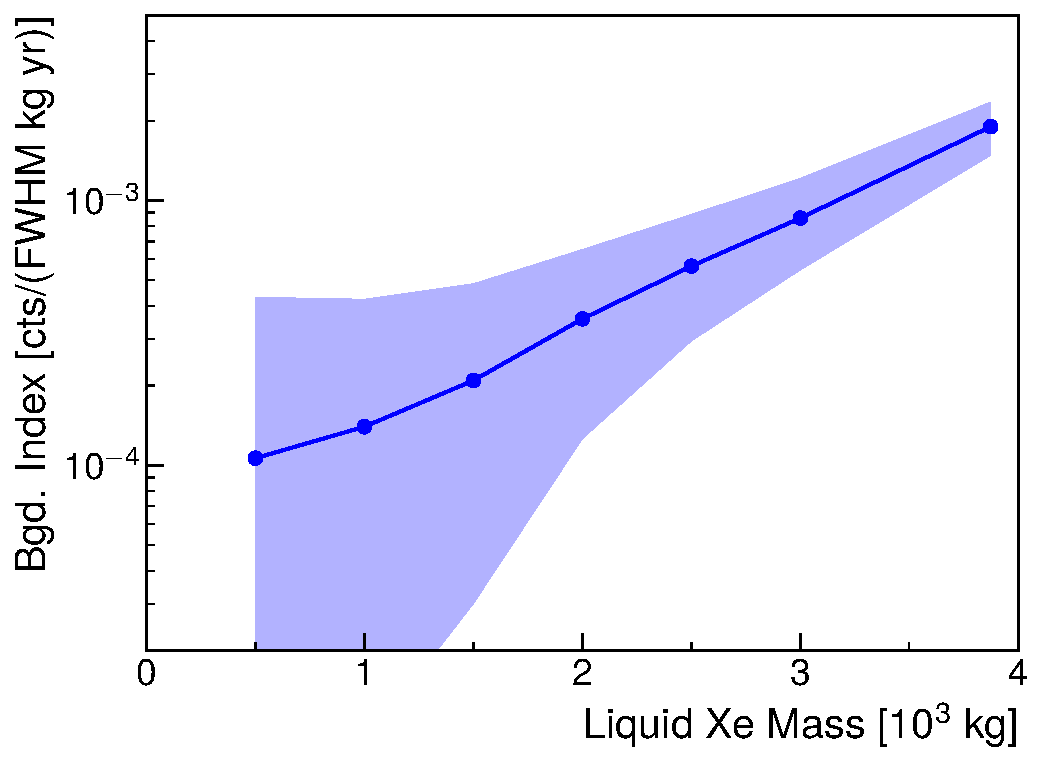
\includegraphics[width=0.6\textwidth]{img/nexo}
%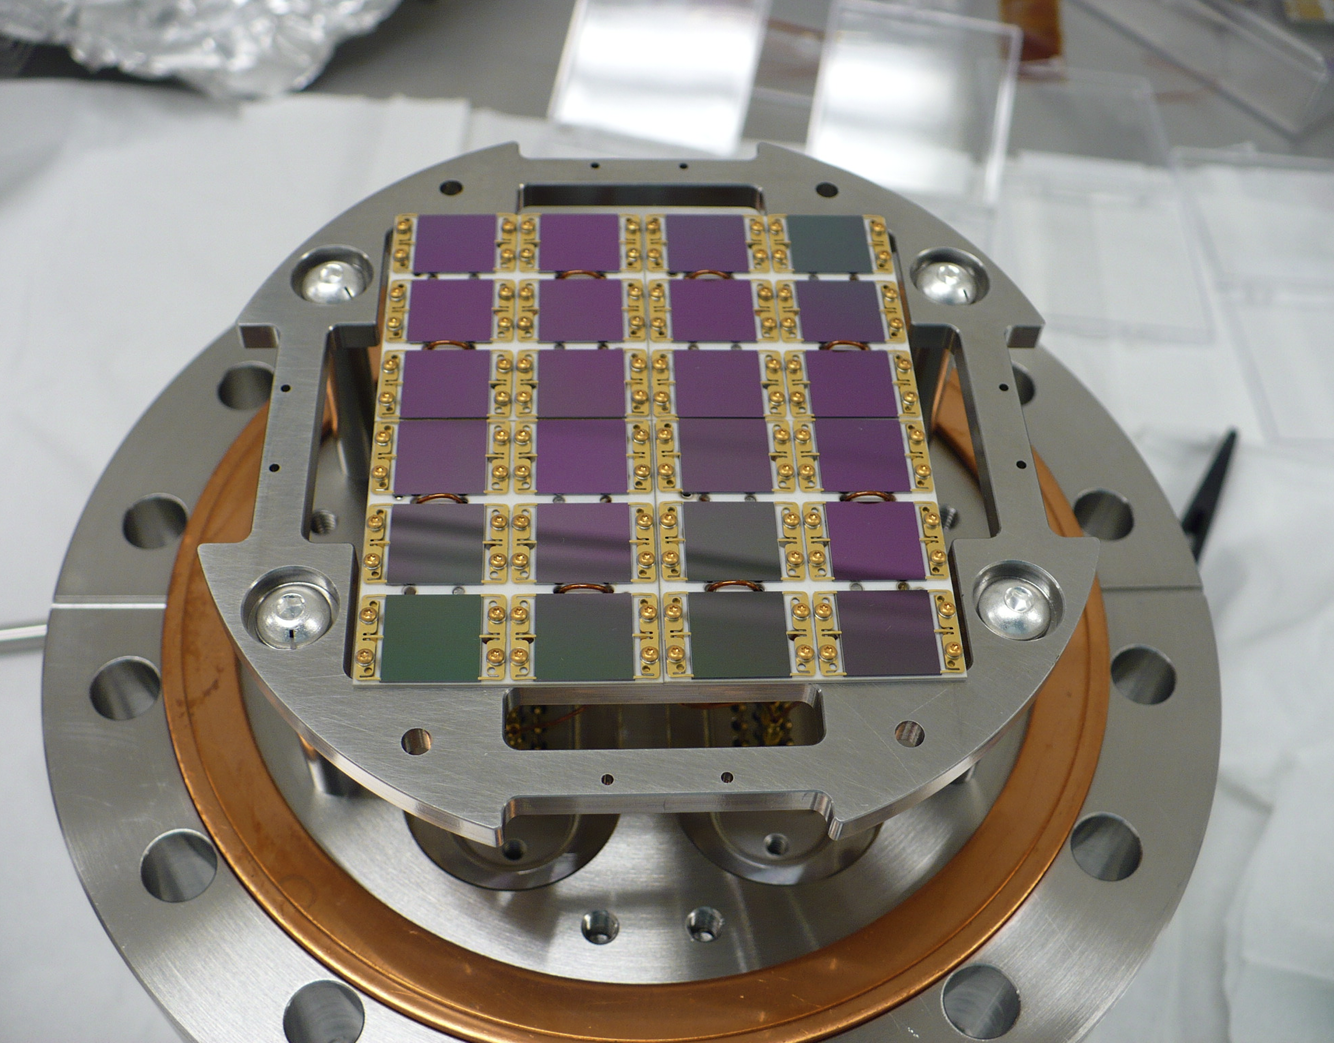
\includegraphics[width=0.475\textwidth]{img/nexo_sipms}
\caption{Expected background index (nEXO simulation) as a function of the active mass of LXe. The plot illustrates the tradeoff in self-shielding calorimeters between background reduction and active mass.} \label{fig:nexo}
\end{figure}

nEXO \cite{nEXO:2018ylp,nEXO:2021ujk}, a follow-on to EXO-200, is a proposed next-generation \bbonu\ experiment with a LXe TPC of 5000~kg of isotopically enriched xenon. It will consist of a single-drift cylindrical TPC 113~cm in diameter and 118~cm in length, holding an active mass of xenon close to 3650~kg. Charge will be collected at the anode with long crossed electrode strips, while a barrel of VUV-sensitive silicon photomultipliers (SiPMs) surrounding the active volume will detect the LXe scintillation light. The TPC vessel, made of copper, will be surrounded by 33~tons of cryogenic fluid, which serves as both thermal bath and radiation shield. nEXO plans to reduce the background rate achieved in EXO-200 to $7\times10^{-5}~\mathrm{counts/(FWHM\cdot kg\cdot yr)}$ taking advantage of the relatively short attenuation length in LXe of $\gamma$ rays of 2.5~MeV, about 8.7~cm, selecting only events occurring in the innermost 2000~kg of the TPC (see fig. \ref{fig:nexo}). The expected energy resolution of the detector is 1.9\% FWHM at 2.5~MeV. This performance results in a projected half-life sensitivity of $1.35\times10^{28}$~years at 90\%CL.
  
\begin{figure}[tb]
\centering
\includegraphics[width=\textwidth]{img/nextTracks.pdf}
\caption{Reconstruction of the trajectories of double electrons (upper row) and single electrons (lower row) produced at the \Tl{208} double escape peak, with energies of 1.6 MeV, recorded in NEXT-White data. Two-electrons deposit energy at the end of each extreme of the track, while single electrons are characterized by a single energy blob. This feature provides a reduction in the background rate of almost two orders of magnitude.} \label{fig:next}
\end{figure}
  
  
NEXT \cite{NEXT:2015wlq, NEXT:2020amj} is an international effort dedicated to the search for \bbonu\ decay in \Xe{136} using high-pressure xenon gas time projection chambers (HPXeTPC) with amplification of the ionization signal by electroluminescence (EL). This detector technology takes advantage of the inherently low fluctuations in the production of ionization pairs (i.e., small Fano factor) in xenon gas to achieve an energy resolution better than 1\% FWHM at \Qbb, significantly better than that of other \Xe{136}-based double-beta decay experiments \cite{Nygren:2009zz}. Moreover, the tracks left in gaseous xenon by \bbonu\ events have distinct features that can be used for background rejection ((see fig. \ref{fig:next}). Over the last decade, the NEXT Collaboration has proven the performance of the HPXeTPC technology in the key parameters required for the observation of \bbonu\ decay, with the underground operation at the Laboratorio Subterr\'aneo de Canfranc of NEXT-{\sc White}, an asymmetric, radiopure HPXeTPC containing approximately 5~kg of xenon at 10~bar pressure. 
The NEXT-100 detector, scheduled to start operation in 2023, constitutes the next phase of the program. It is an asymmetric HPXeTPC containing about 100~kg of xenon (enriched at $\sim$90\% in \Xe{136}) at 15~bar. NEXT-100 will reach a sensitivity of about $6\times10^{25}$~year after a run of 3 effective years, for a predicted background index of at most $4\times10^{-4}$ \ckky. A scaled-up version of this technology, dubbed NEXT-HD, with about 1 tonne of enriched xenon, could reach in less than 5 years of operation a sensitivity to the half-life of \bbonu\ decay better than $10^{27}$~years, significantly improving over current limits. 

Xenon TPCs can, potentially, detect (``tag") the daughter $Ba^{2+}$ cation emitted in the \bbonu\ decay of \Xe{136}, in (delayed) coincidence with the two beta electrons. 
The possibility of barium tagging in a xenon TPC was proposed in 1991\cite{Moe:1991ik} and relied on Ba$^+$ fluorescence imaging using two atomic excitation levels in very low density gas. Recently,
the nEXO collaboration has demonstrated the imaging and counting of individual barium atoms in solid xenon by scanning a focused laser across a solid xenon matrix deposited on a sapphire window \cite{nEXO:2018nxx}. This is a promising step for barium tagging in liquid xenon, where recombination is frequent, and the barium daughters are distributed across charge states from 0 to 2$^+$ \cite{PhysRevC.92.045504}, with sizeable populations of neutral Ba and  Ba$^+$.  

In high pressure gas phase, on the other hand, recombination is minimal \cite{1997NIMPA.396..360B}, and $Ba^{2+}$ dominates. In 2015, a promising technique to detect $Ba^{2+}$ in a HPXe, using a layer of molecular indicators was
proposed \cite{Nygren:2015xxi}. The concept was further developed in \cite{Jones:2016qiq} and spanned a vigorous R\&D program within the NEXT collaboration \cite{McDonald:2017izm,Rivilla:2020cvm}. 
Daughter ion tagging is undoubtedly very challenging from the technical point of view, but the payoff ---the potential to operate in the ``background free'' limit--- for future \bbonu\ experiments aiming at sensitivities of $10^{28}$ year and beyond  would be huge.

\subsection{Loaded liquid scintillator} 
\label{subsec:liquid_scint}
%
Large liquid scintillator detectors such as SNO \cite{SNO:2002tuh}, KamLAND \cite{KamLAND:2002uet} or Borexino \cite{Borexino:2008gab} have a successful track record in low-background searches in neutrino physics. Loading them with large amounts of \bb\ isotopes represents a cost-effective way to search for neutrinoless double beta decay. Two collaborations are pursuing this approach: KamLAND-Zen and SNO+. Both experiments are reusing the existing detector infrastructure from previous reactor and solar neutrino experiments. 

The KamLAND-Zen experiment \cite{} is seaching for the \bbonu-decay of \Xe{136} using enriched xenon dissolved in liquid scintillator, a technique first proposed in 1994 \cite{Raghavan:1994qw}. The experiment reuses the neutrino KamLAND detector, located at the Kamioka Observatory, Japan. The KamLAND-Zen detector is composed of two concentric transparent balloons. The inner one, 3.8~m diameter and fabricated from 25 $\mu$m thick nylon film, contains 13 tonnes of liquid scintillator loaded with 745~kf of enriched xenon. The outer balloon, 13~m in diameter, contains 1~kilotonne of pure liquid scintillator, and serves as an active shield for external gamma background as well as a detector for internal radiation from the inner balloon. Buffer oil between the outer balloon and an 18~m diameter spherical stainless-steel containment tank shields the detector from external radiation. Scintillation light is recorded by 1325 17-in and 554 20-in photomultiplier tubes mounted on the stainless-steel tank, providing 34\% solid-angle coverage. The containment tank is surrounded by a 3.2-kt water-Cherenkov outer detector. KamLAND-Zen, which has been collecting physics data since late 2011, has published a measurement of the half-life of the \bbtnu\ decay of \XE, $2.38\pm0.02~(\mathrm{stat})\pm0.14~(\mathrm{syst})\times10^{21}$~years \cite{KamLANDZen:2012aa}, and a limit to the half-life of the \bbonu\ decay, $2.3\times10^{26}$~years (90\% CL)~\cite{KamLAND-Zen:2022tow,}. The energy resolution of the detector is 9.9\% FWHM at the $Q$ value of \XE. The achieved background rate in the region of interest is approximately $1.4\times10^{-4}$~\ckky, thanks to a tight selection cut in the fiducial volume and the identification of $^{214}$Bi events via Bi-Po tagging. KamLAND-Zen continues taking data, aiming at a sensitivity of $4.6\times10^{26}$~yr. The collaboration is planning a future upgrade to increase the photocathode coverage and improve light collection, which would allow them to reach energy resolutions close to 5\% (FWHM) at the \Qbb\ value. 

SNO+, the follow-up of the \emph{Sudbury Neutrino Observatory} (SNO), is a multipurpose liquid scintillator experiment housed in SNOLAB (Ontario, Canada). The detector reuses many of the components of its predecessor, replacing the heavy water by 780~tonnes of liquid scintillator in order to obtain a lower energy threshold. The detector consists of a 12~m diameter acrylic vessel surrounded by about 9500 8-in photomultiplier tubes that provide a 54\% effective photocathode coverage. The acrylic vessel is immersed in a bath of ultra pure water that fills the remaining extent of the underground cavern, attenuating the background from external media such as the PMTs and surrounding rock. The density of the liquid scintillator (0.86~g/cm$^{3}$) being lower than that of the surrounding water leads to a large buoyant force on the acrylic vessel. To keep it in place, a hold-down rope net has been installed over the detector and anchored to the cavity floor. The ultimate physics goal of the SNO+ experiment is to conduct a search for \bbonu\ in \Te{130}, which will be loaded into the liquid scintillator in the form of (non-enriched) telluric acid. A loading of 0.5\%, equivalent to 1.3~tons of \TE, is planned for the first phase of the experiment. The energy resolution of the SNO+ detector is expected to be 10.5\% FWHM at the $Q$ value of \TE. Consequently, the \bbtnu\ spectrum will be an important source of background. The expected levels of uranium and thorium in the liquid scintillator can also result in substantial activity near the \bbonu\ endpoint, mostly from the decays of $^{214}$Bi and $^{212}$Bi. Nevertheless, these can be, in principle, actively suppressed via Bi-Po $\alpha$ tagging. External backgrounds (not originating in the liquid scintillator) can be suppressed with a tight fiducial volume selection.



% \subsection{Past experiments} \label{subsec:past} 
% %%%%%
For almost half a century the only evidence of the existence of double beta decay came from geochemical methods consisting in measuring the concentrations of the stable daughter isotopes $(Z+2,A)$, produced over geologic times ($\sim 10^9$ years). An excess of the daughter isotope over its natural concentration is interpreted as evidence for \bb\ decay (either \bbtnu\ or \bbonu, since the method cannot distinguish between them).

The first direct measurement of \bbtnu, in \SE, did not happen until 1987 \cite{Elliott:1987kp}. It was done using a fairly large ($\sim1$ m$^{3}$) time projection chamber, the well-known Irvine TPC. The source, 14 g of 97\% enriched \SE, was deposited on a thin Mylar foil forming the central electrode of the chamber. The trajectories of the electrons emitted from the source foil were recorded by the TPC and analyzed to infer their energy and kinematic characteristics. Since this initial detection, the two-neutrino mode has been directly observed for 8 isotopes in several experiments (see table \ref{tab:bb2nu_exp} and ref.~\cite{Barabash:2010ie} for further details).

The most restricting limits to date in the search for \bbonu\ were obtained with germanium detectors. The Heidelberg-Moscow (HM) experiment \cite{Klapdor-Kleingrothaus:2000eir} searched for the \bbonu\ decay of \GE\ using five high-purity Ge semiconductor detectors enriched to 86\% in \GE. The experiment ran in the Laboratori Nazionali del Gran Sasso (LNGS), Italy, from 1990 to 2003, totaling an exposure of 71.7 kg$\cdot$year. The background rate reached by the experiment in the \Qbb\ region was ($0.19\pm 0.01$) \ckky, or, in units of \bb\ emitter mass, $0.22\pm 0.01$ \ckkbby. Pulse shape discrimination (PSD) was used in a subset of the data (35.5 kg$\cdot$year) to separate single-site events, like \bbonu\ decays, from multi-site events, like $\gamma$ interactions, resulting in a background rate of ($0.06\pm 0.01$) \ckky, or ($0.07\pm 0.01$) \ckkbby. A lower limit on the \bbonu\ half-life of $T^{0\nu}_{1/2}(\GE) \geq 1.9 \times 10^{25}$ years (90\% CL) was obtained \cite{Klapdor-Kleingrothaus:2000eir}.

A subset of the collaboration re-analyzed the data claiming evidence for \GE\ \bbonu\ decay \cite{Klapdor-Kleingrothaus:2001oba}. The latest publication by this group reports a $6\sigma$ evidence for \bbonu\ and a half-life measurement of $T_{1/2}^{0\nu}=(2.23^{+0.44}_{-0.31})\times 10^{25}$ years \cite{Klapdor-Kleingrothaus:2006zcr}, corresponding to $\mbb\ = (0.30^{+0.02}_{-0.03})\ \text{eV}$ according to the central value of the PMR nuclear matrix element for \GE\ given in sect.~\ref{subsec:nme_pmr}. This claim sparked an intense debate in the community, and at the moment no consensus exists about its validity (see, for example, ref.~\cite{Aalseth:2002dt}).

The International Germanium Experiment (IGEX) \cite{IGEX:2002bce} also searched for \bbonu\ using enriched germanium crystals. It ran in the Homestake gold mine (USA), the Canfranc Underground Laboratory (Spain) and the Baksan Neutrino Observatory (Russia) from 1991 to 2000, accumulating a total exposure of 8.87 kg$\cdot$year. It reached a sensitivity similar to that of Heidelberg-Moscow, but not enough to disprove the claim. The lowest background rate reached by the IGEX experiment was 0.26 (0.10) \ckky\ without (with) pulse shape discrimination for a 8.87 (4.65) kg$\cdot$year total exposure \cite{Gonzalez:2003pr}, corresponding to 0.30 (0.12) \ckkbby\ per unit \bb\ emitter mass.

The Cuoricino experiment, an array of 62 TeO$_{2}$ bolometric crystals, ran for five years in Gran Sasso searching for \bbonu\ in \TE. It reached a sensitivity to \mbb\ comparable to that of the HM experiment, but it cannot disprove the claim due to the uncertainties in the nuclear matrix elements. The average background rate for the 5$\times$5$\times$5 cm$^3$ Cuoricino crystals, computed in a 60 keV wide region centered around \Qbb , was $0.161\pm 0.006$ \ckky\ \cite{CUORE:2011boi}, corresponding to $0.58\pm 0.02$ \ckkbby\ per unit \bb\ emitter mass. The average FWHM energy resolution in all crystals was $6.3\pm 2.5$ keV at 2615 keV \cite{CUORE:2011boi}.

The lowest levels of background so far were achieved by the NEMO3 experiment \cite{NEMO:2009ewu}: a few times $10^{-3}$ \ckky . This detector represents the state of the art of separate-source \bb\ experiments. Reconstruction of the electron tracks emerging from the source provided a powerful signature to discriminate signal from background. The NEMO3 experiment ran from 2003 to 2010 at the Modane Underground Laboratory (LSM), in France. The detector, of cylindrical shape, had 20 segments of thin source planes, with a total area of 20 m$^{2}$, supporting about 10 kg of source material. The sources were within a drift chamber, for tracking, surrounded by plastic scintillator blocks, for calorimetry. A solenoid generated  a magnetic field of 25 Gauss which allowed the measurement of the tracks electric charge sign. The detector was shielded against external gammas by 18 cm of low-background iron. Fast neutrons from the laboratory environment were suppressed by an external shield of water, and by wood and polyethylene plates. The air in the experimental area was constantly flushed, and processed through a radon-free purification system embedding the detector volume. In addition to searching for \bbonu , NEMO3 very successfully served as a ``\bbtnu\ factory'', providing precise \bbtnu\ half-life measurements for seven \bb\ isotopes, see table \ref{tab:bb2nu_exp}. Apart from representing the ultimate background for \bbonu\ searches , an accurate measurement of \bbtnu\ in several nuclides is also important as input to NME calculations. 

% \subsection{CUORE} \label{subsec:cuore}
% The Cryogenic Underground Observatory for Rare Events (CUORE) \cite{Ardito:2005ar}
has been designed following the successful experience of the  MiDBD \cite{Arnaboldi:2002te} and Cuoricino \cite{Andreotti:2010vj} $^{130}$Te experiments, where for the first time arrays of bolometers were used to search for $\beta\beta$ decay.

CUORE will be placed in the hall A of the Gran Sasso Underground Laboratory and will consist of a system of 988 bolometers, each being a crystal of TeO$_2$ of $5\times5\times5$ cm$^3$, arranged in 19 vertical towers consisting of 13 layers of 4 crystals each. The four crystals are held between two copper frames joined by copper columns. PTFE pieces are inserted between the copper and TeO$_2$, as a heat impedance and to clamp the crystals. There is a few mm gap between crystals with no material between them.
A system of lead shields will be hosted inside the cryostat close to the detectors, to shield them from environmental radioactivity and from radioactive contaminations originating in the dilution unit located above the detector and in the dewar structure \cite{Bellini:2007zz}. A 6 cm thick roman lead shield surrounds the detector array on its sides, while a 30 cm thick layer of low-activity lead is placed above the detector. The $^{210}$Pb activity of the roman lead was measured to be less than 4 mBq/kg. A sketch of the detector is shown in fig.~\ref{fig:cuore}.

%%%%%
\begin{figure}[t!]
\begin{center}
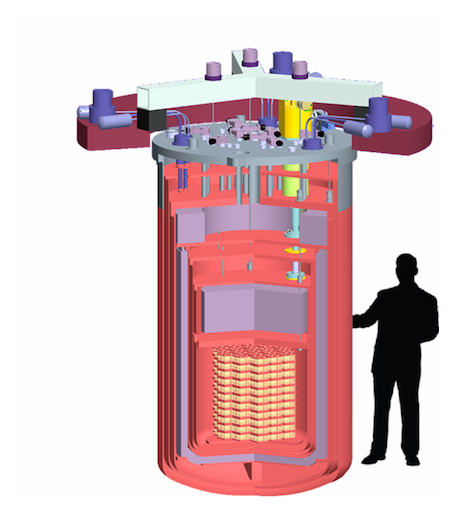
\includegraphics[scale=.8]{img/cuore.eps}
\end{center}
\caption{The CUORE detector and cryostat. In yellow, the 19 towers of bolometers; the lavender volumes are the lead shielding.}\label{fig:cuore}
\end{figure}
%%%%%

The total mass of the detector will be 741 kg for a $^{130}$Te mass of 206 kg. The energy released in a single particle interaction within the crystal is measurable as a change in temperature by  Neutron Transmutation Doped (NTD) germanium thermistors. The measured energy resolution is $\sim 5$ keV FWHM at the $\beta \beta \; (0\nu)$ transition energy ($\sim 2.53$ MeV).

The CUORE bolometers will operate at temperatures between 10 and 15 mK. A challenging $^3$He/$^4$He dilution refrigerator, with a cooling power of 3 mW at 120 mK, has been designed on purpose and is under construction.

A single tower of CUORE, CUORE-0, is presently under construction and will begin  operations within 2011. It will be hosted in the old Cuoricino dilution refrigerator, placed in the hall A of the LNGS. CUORE-0 is a real test of the CUORE assembly chain and procedure, will directly test the level of backgrounds of the CUORE setup and improve the Cuoricino sensitivity on \bbonu.

The CUORE setup will possibly allow in the long term for powerful upgrades. An obvious, though expensive, possibility is to substitute the natural tellurium bolometers with enriched $^{130}$Te units (provided that the enrichment procedure can keep the internal backgrounds very low). A more sophisticated option is to use scintillating crystals containing interesting double beta emitters \cite{Pirro:2005ar}. The contemporary read-out of scintillation light and thermal signal could indeed allow for a dramatic reduction of the background rate and a better characterization of the signal. An array of ZnSe scintillating bolometers, LUCIFER, has been recently proposed as a prototype experiment exploring the performances of such an approach \cite{Ferroni:2011zz} (see sect.~\ref{subsec:other}).




% \subsection{nEXO} \label{subsec:exo}
% %The Enriched Xenon Observatory \cite{Hall:2010zzg} will search for \bbonu\ in \XE. The ultimate goal of the Collaboration is the development of the barium tagging for a multi-ton xenon-based detector, which would lead to a virtually background-free experiment. Prior to that, the Collaboration has built the EXO-200 detector, a $\sim$200-kg liquid xenon (enriched to 80.6\% in \XE) time projection chamber that detects both scintillation and ionization.
%
%The fiducial volume of the chamber, 44 cm in length, is divided in two halves by a central cathode (see fig.~\ref{fig:exo}, left). Ionization charges created in the xenon by charged particles drift under the influence of an electric field towards the two ends of the chamber. There, the charge is collected by a pair of crossed wire planes which measure its amplitude and transverse coordinates. Each end of the chamber includes also an array of avalanche photodiodes (APDs) to detect the 178-nm scintillation light produced by primary interactions. The sides of the chamber are covered with teflon sheets that act as VUV reflectors, improving the light collection. The simultaneous measurement of both the ionization charge and scintillation light of the event may in principle allow to reach a detector energy resolution as low as 3.3\% FWHM at the \XE\ Q-value, for a sufficiently intense drift electric field \cite{EXO-200:2003bso}. 
%
%The xenon is held inside a thin copper vessel immersed in a cryofluid that also shields the experiment from external radioactive backgrounds. The HFE heat-transfer fluid is stored in a vacuum-insulated low-activity copper cryostat. The cryostat is surrounded on all sides by 25 cm of low-activity lead. The entire assembly is surrounded by a radon-free tent and housed in a class 100 clean room, the exterior of which is instrumented on five sides with plastic scintillator panels for vetoing cosmic rays with 95.9\% efficiency. The detector is located 2150 feet underground for an overburden of 1585 meters water equivalent, at WIPP (Waste Isolation Pilot Plant), in the United States.
%
%%%%%%
%\begin{figure}[t!]
%\begin{center}
%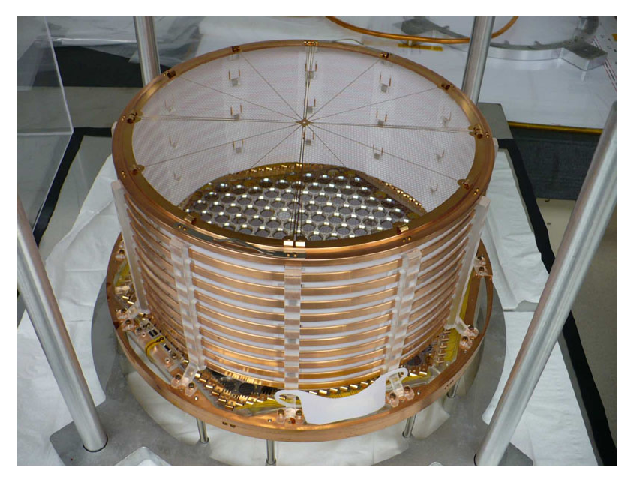
\includegraphics[width=0.475\textwidth]{img/exo1.eps}
%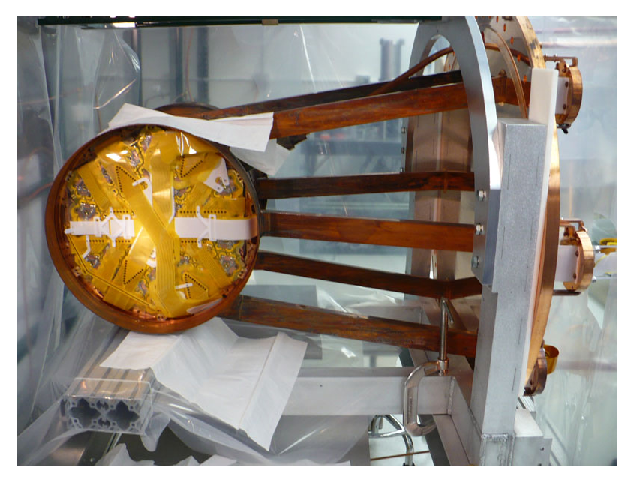
\includegraphics[width=0.475\textwidth]{img/exo2.eps}
%\end{center}
%\caption{Left: one half of the EXO chamber, viewed from the cathode plane. Right: the chamber attached to the cryostat door, as viewed from the bottom of the APD plane. The legs contain the readout cabling and are also the conduits for xenon circulation.} \label{fig:exo}
%\end{figure}
%%%%%%
%
%The EXO-200 TPC was installed in its cryostat in early 2010. The detector was first filled with natural (unenriched) xenon in late 2010. The data collected during these engineering runs were used to make a first assessment of the performance of the detector, and to perform a first round of calibrations. Low-background running with enriched xenon started in the spring of 2011. The EXO Collaboration announced the observation of the \bbtnu\ mode of \XE\ in August 2011. Prior to this measurement, reported in table~\ref{tab:bb2nu_exp}, the \bbtnu\ had been observed in all other important \bbonu\ candidate nuclei except \XE . The measured \bbtnu\ half-life is significantly lower than previously reported lower limits \cite{Bernabei:2002bn,Gavriljuk:2005xc}.
%
%To identify the daughter barium, several methods are under study, including single-ion fluorescence, resonant ionization spectroscopy (RIS), and mass spectroscopy. Single ion fluorescence is a highly sensitive and highly selective method to observe a barium ion while held under vacuum in a RF trap. In this technique, the Ba$^+$ ion is rapidly cycled from its $6^2\text{S}_{1/2}$ ground state to its $6^2\text{P}_{1/2}$ excited state by illuminating it with lasers of the appropriate wavelength (493 nm and 650 nm), see fig.~\ref{fig:bariumenergylevels}. As the electronic state changes, the laser photons are scattered in all directions, and the scattered light can be easily detected by a photo-multiplier tube. EXO has achieved good single barium ion identification with this technique, even in the presence of low pressure xenon and helium gas mixtures. However, this technique also requires that the barium ion be retrieved from the TPC volume, transported to the RF trap, released, and trapped, while not altering its chemical or ionization state. Resonant ionization spectroscopy, on the other hand, is a technique which allows single barium ions to be observed without requiring a vacuum ion trap. In RIS, barium ions are desorbed from the surface of a transport probe, and subsequently resonantly ionized under illumination by 554 nm and 390 nm lasers. The ionized barium can then be observed with a Channeltron electron multiplier. Initial tests with the RIS technique have successfully identified barium being desorbed from the probe tip, so this technique is promising. Other avenues of research include barium identification within xenon ice, and barium extraction from a high pressure gas TPC using gas nozzles. 
% 


The nEXO neutrinoless double beta decay experiment is designed to use a time projection chamber and 5000 kg of isotopically enriched liquid xenon to search for the decay in 136Xe. This detector will be based on very successful EXO-200 detector. A single-phase liquid xenon TPC instrumented to read both scintillation and charge. The anti-correlation of these two signals allowed for an energy resolution of 2.89\% FWHM@Qbb \cite{EXO-200:2020wmu}.

This design also provided the capability of a good fidutialization of the events in the detector and, more important, certain capability to separate them by topology. In particular, the separation of single-site and multi-site events [cite] provided a strong background suppression.

The nEXO design aims to build a volume of 5 tonnes of enriched Xe136. The TPC vessel is a right copper cylinder with both inner height and diameter equal to 127.7 cm surrounded by 33,000 kg of HFE-7000, which serves as both thermal bath and radiation shield. A vacuum layer between an inner vessel and an outer vessel of the cryostat provides thermal insulation from an active water shield, referred to as the outer detector. The TPC itself will have 113.3 cm diameter by 118.3 cm drift height, creating a total xenon mass in the drift region of 3648 kg for an active mass of 3281 kg. This design requires 10 ms of electron life-time to guarantee good energy resolution when reading the ionisation signal. This is achieve by a good purification system and a relatively moderate drift field of 400 V/cm. \cite{nEXO:2021ujk}.



%%%%%%
\begin{figure}[t!]
\begin{center}
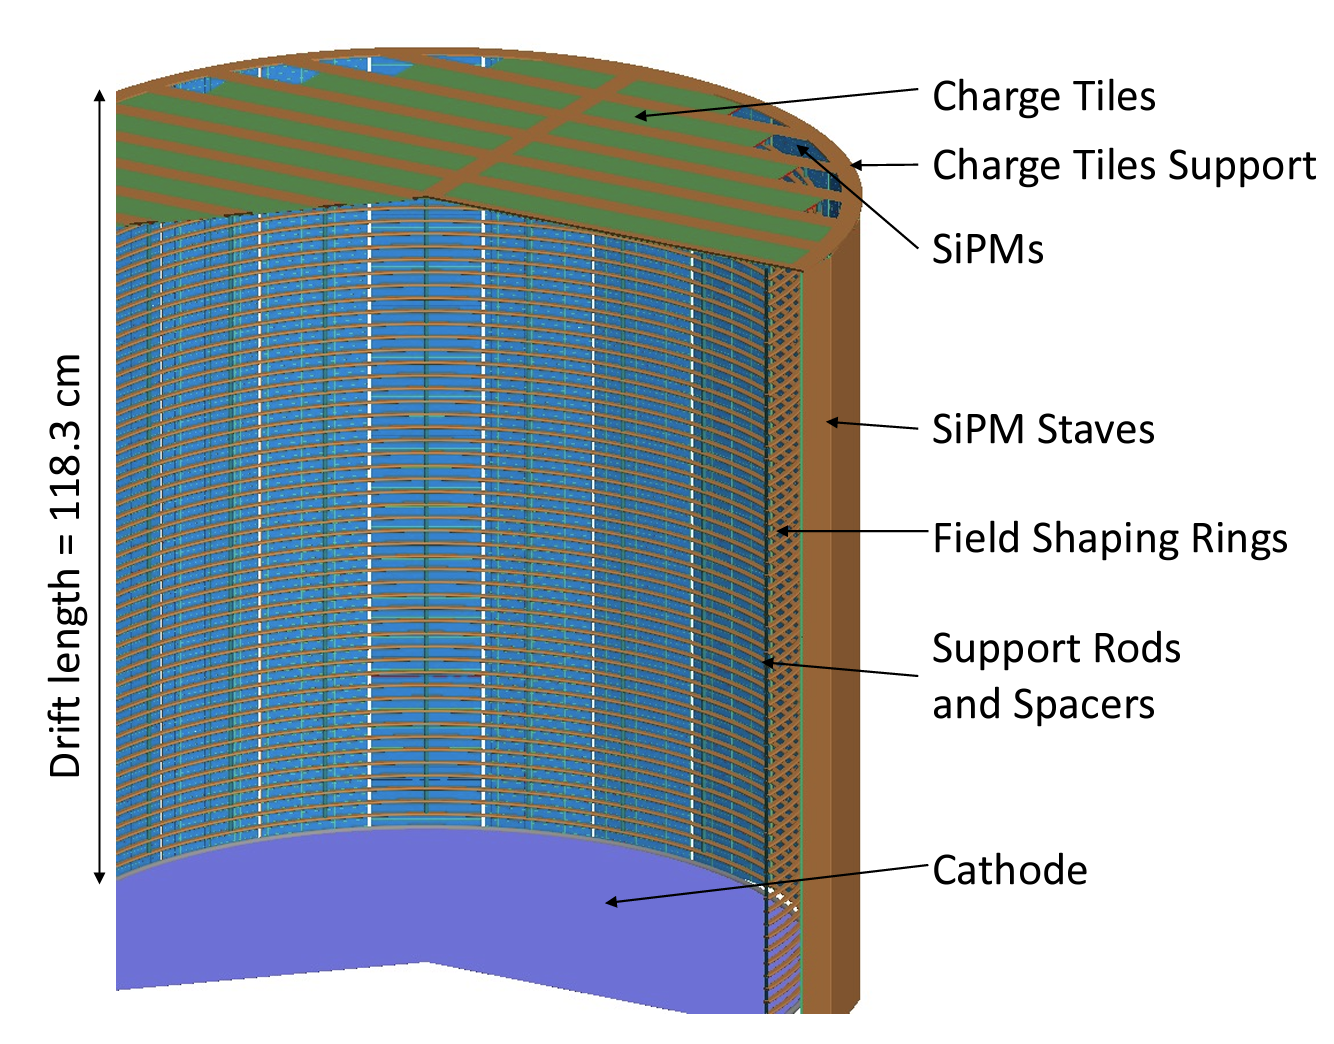
\includegraphics[width=0.475\textwidth]{img/nexo_design}
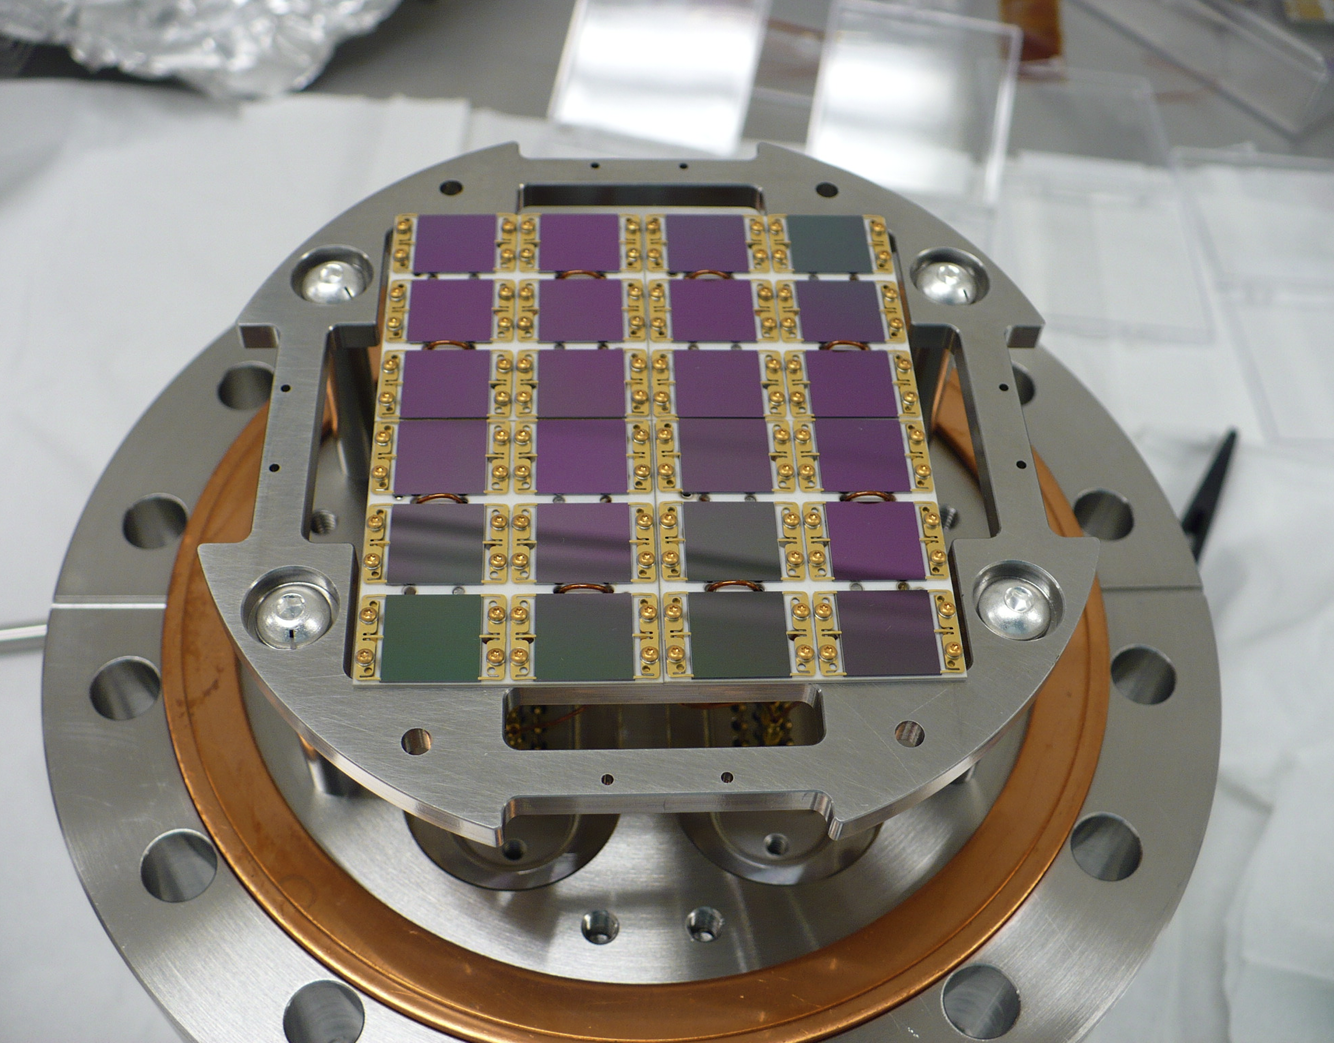
\includegraphics[width=0.475\textwidth]{img/nexo_sipms}
\end{center}
\caption{Left: Close up view of the main components inside the nEXO TPC vessel. Right: Test array of 24 SiPMs used to be used together with charge collection tiles in LXe.Each SiPM is cm$^2$.} \label{fig:nexo}
\end{figure}

Efficient scintillation light collection is an essential requisite for nEXO to attain proper energy resolution and to provide the start time to localize events along the drift field. Actually, in order to reach <2.35\% FWHM energy resolution, the overall optical efficiency must be 3\%  or higher, this is achieved by using SiPMs arrays operated directly in the liquid xenon behind the TPC field shaping rings. The SiPM will have ~1cm$^2$ active area and will be mounted in 24 long staves surrounding the TPC field cage. The necessity of reading as much light as possible has a relevant impact on the TPC design. In particular, the field cage must be as transparent as possible allowing the photons to reach the photsensors region. This affect the geometry of the rings, as they need to be thiner. Also, a coating of vacuum deposited aluminum, protected against oxidation by a layer of MgF2 will make all rings reflective to VUV. In addition, it will allow to remove the traditional PTFE reflective panels used in other liquid xenon TPCs, thus reducing the amount of materials and outgassing inside the detector volume.

One of the main tools the nEXO collaboration proposes to reduce the level of background events is the based on taking advantage of the relatively short attenuation length of $\gamma$-ray at 2.4 MeV energy in LXe, of only 8.7 cm. By selecting a region in the most inner part of the detector they can further reduce the background rate by almost an order of magnitude in the most inner ton of active material. Adding this technique to the energy resolution and topological separation nEXO is predicted to achieve a background rate of 3.6 × 10$^{-4}$ cts/(FWHM·kg·y) in the inner 2000 kg of LXe. 

With this level of background nEXO aims to reach a sensitivity of 9.2 × 10$^{27}$ yrs at 90\% C.L. after 10 years of operation and, an expected 3 sigma discovery potential of 5.7 × 
10$^{27}$ yrs \cite{nexocprecdr}. However, in a recent document \cite{nEXO:2021ujk} the nEXO Collaboration claims for an improved design and understanding of the nEXO design, together with the development of a \bbonu\ DNN discriminator that pushes the background index to 
b=7×10$^{-5}$ cts/(FWHM·kg·yr) obtaining a half-life sensitivity of 1.35×10$^{28}$ 
yr at 90\% C.L.

% \subsection{GERDA} \label{subsec:gerda}
% The GERmanium Detector Array (GERDA) experiment \cite{Abt:2004yk}, located in Hall A of the Laboratori Nazionali del Gran Sasso (LNGS), will make use of naked Ge detectors immersed in a large cryostat of ultra-pure LAr.

The Ge detectors are organized in strings (2--5 detectors) and mounted in special low-mass ($\sim 80$ g) holders made of ultra-pure copper and PTFE. The array of strings is contained in a vacuum insulated stainless steel cryostat of 4.2 m diameter and 8.9 m height. A copper shield covers the inner cylindrical shell of the cryostat with a maximum thickness of 6 cm. The cryostat is placed in a water tank, of 10 m diameter and 9.4 m height, serving as a gamma and neutron shield. It will be also used as a veto against cosmic rays thanks to its instrumentation with 66 photomultipliers, with good efficiency in detecting the Cherenkov light. The cosmic muon veto is reinforced by plastic scintillator panels on top of the detector, for a surface of about 20 m$^2$. A drawing of the detector and shielding is shown in fig.~\ref{fig:gerda}.

%%%%%
\begin{figure}[t!]
\begin{center}
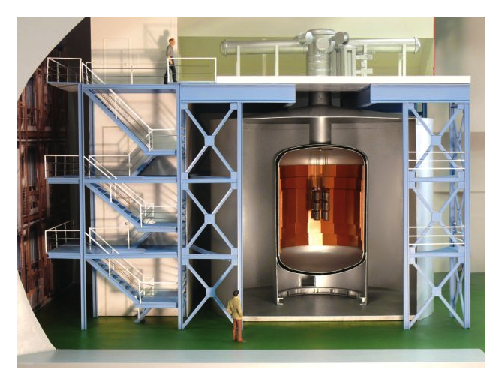
\includegraphics[]{img/gerda.eps}
\end{center}
\caption{Sketch of the GERDA experiment. The germanium arrays can be seen inside the copper cryostat, and this one placed inside the cylindrical water tank.} \label{fig:gerda}
\end{figure}
%%%%%

In its first phase, GERDA-1, eight fully refurbished germanium diodes (17.7 kg total active mass, 86\% isotopic enrichment in \GE ) from the previous Heidelberg-Moscow and IGEX experiments will be used. In the subsequent step, GERDA-2, new diodes will be used for a total active mass of 35.4 kg. These new diodes will be p-type Broad Energy (BEGe) detectors \cite{Budjas:2008wb,Agostini:2010ke}, allowing for a better discrimination of backgrounds thanks to a sophisticated pulse shape discrimination.

The experiment started commissioning runs in June 2010 using natural Ge, low-background, detectors, refurbished from the Genius-TF experiment. These commissioning runs focused on the investigation of the background sources (most notably on the unexpectedly large contribution from $^{42}$Ar-$^{42}$K in the LAr) and on $^{42}$Ar background mitigation strategies, see sect.~\ref{subsec:sensi_assumptions}. Data taking for the GERDA-1 physics run will start in the next months. The background level of the natural Ge setup was measured to be $0.06\pm 0.02$ \ckky\ (corresponding to $0.07\pm 0.02$ \ckkbby ), consistent with early indications from the first string of enriched Ge detectors deployed \cite{Cattadori:2012fy}. This rate, obtained without using pulse shape information, is a factor of 3--4 lower than the HM and IGEX measured ones (see sect.~\ref{subsec:past}), but still about a factor of 6 higher than the GERDA-1 goal. The reason for this higher than expected background rate is at present not fully understood. The goals of GERDA-2 are to start data taking in about two years, with about twice the isotope mass of GERDA-1, and with a background level of 0.001 \ckky\ (or 0.0012 \ckkbby ).

In the very long term a third phase of the experiment, GERDA-3, is foreseen to make use of about 1 ton of $^{76}$Ge target material together with a further reduction of background. Such an effort, common with the MAJORANA project (see below), would be feasible only in a word-wide collaboration, and provided that the GERDA approach could demonstrate to be the best candidate technology to push the double beta decay sensitivity below the inverted hierarchy mass threshold (about 30 meV). 
 

% \subsection{MAJORANA} \label{subsec:majorana}
% The MAJORANA Collaboration is following a more classic approach than GERDA in the design of a germanium-based experiment \cite{Majorana:2011rit}. The Ge detectors will be mounted in a string-like arrangement in ultra-pure vacuum cryostat made from radiopure copper. The cryostat will be surrounded by a passive shielding of Cu and Pb, and an active muon veto.

The Collaboration is building a demonstrator module, to be placed at the Deep Underground Science and Engineering Laboratory (DUSEL) in the United States, with about 20 kg of natural BEGe detectors. The goal is to demonstrate a background rate of about 4 counts per tonne and per year in the 4-keV wide region of interest \cite{Majorana:2011vap}. The demonstrator is expected to operate with enriched detectors in 2013.
 

% \subsection{KamLAND-Zen} \label{subsec:kamland}
% %The KamLAND-Zen experiment will search for \bbonu\ in \XE\ using enriched xenon dissolved in liquid scintillator. This will allow a calorimetric measurement of the \bb\ electrons, as first proposed in \cite{Raghavan:1994qw}. Xenon is relatively easy to dissolve (with a mass fraction of more than 3\% being possible) and also easy to extract from the scintillator. 

%The major modification to the existing KamLAND detector \cite{KamLAND:2002uet} was the construction of an inner, very radiopure (of order $3\times 10^{-12}$ g/g of \URANIUM\ and \THORIUM) and very transparent balloon to hold the dissolved xenon. This balloon, 1.58 m in radius, is placed at the center of the KamLAND active volume as shown in fig.~\ref{fig:kamlandzen}.

%%%%%
%\begin{figure}[t!]
%\begin{center}
%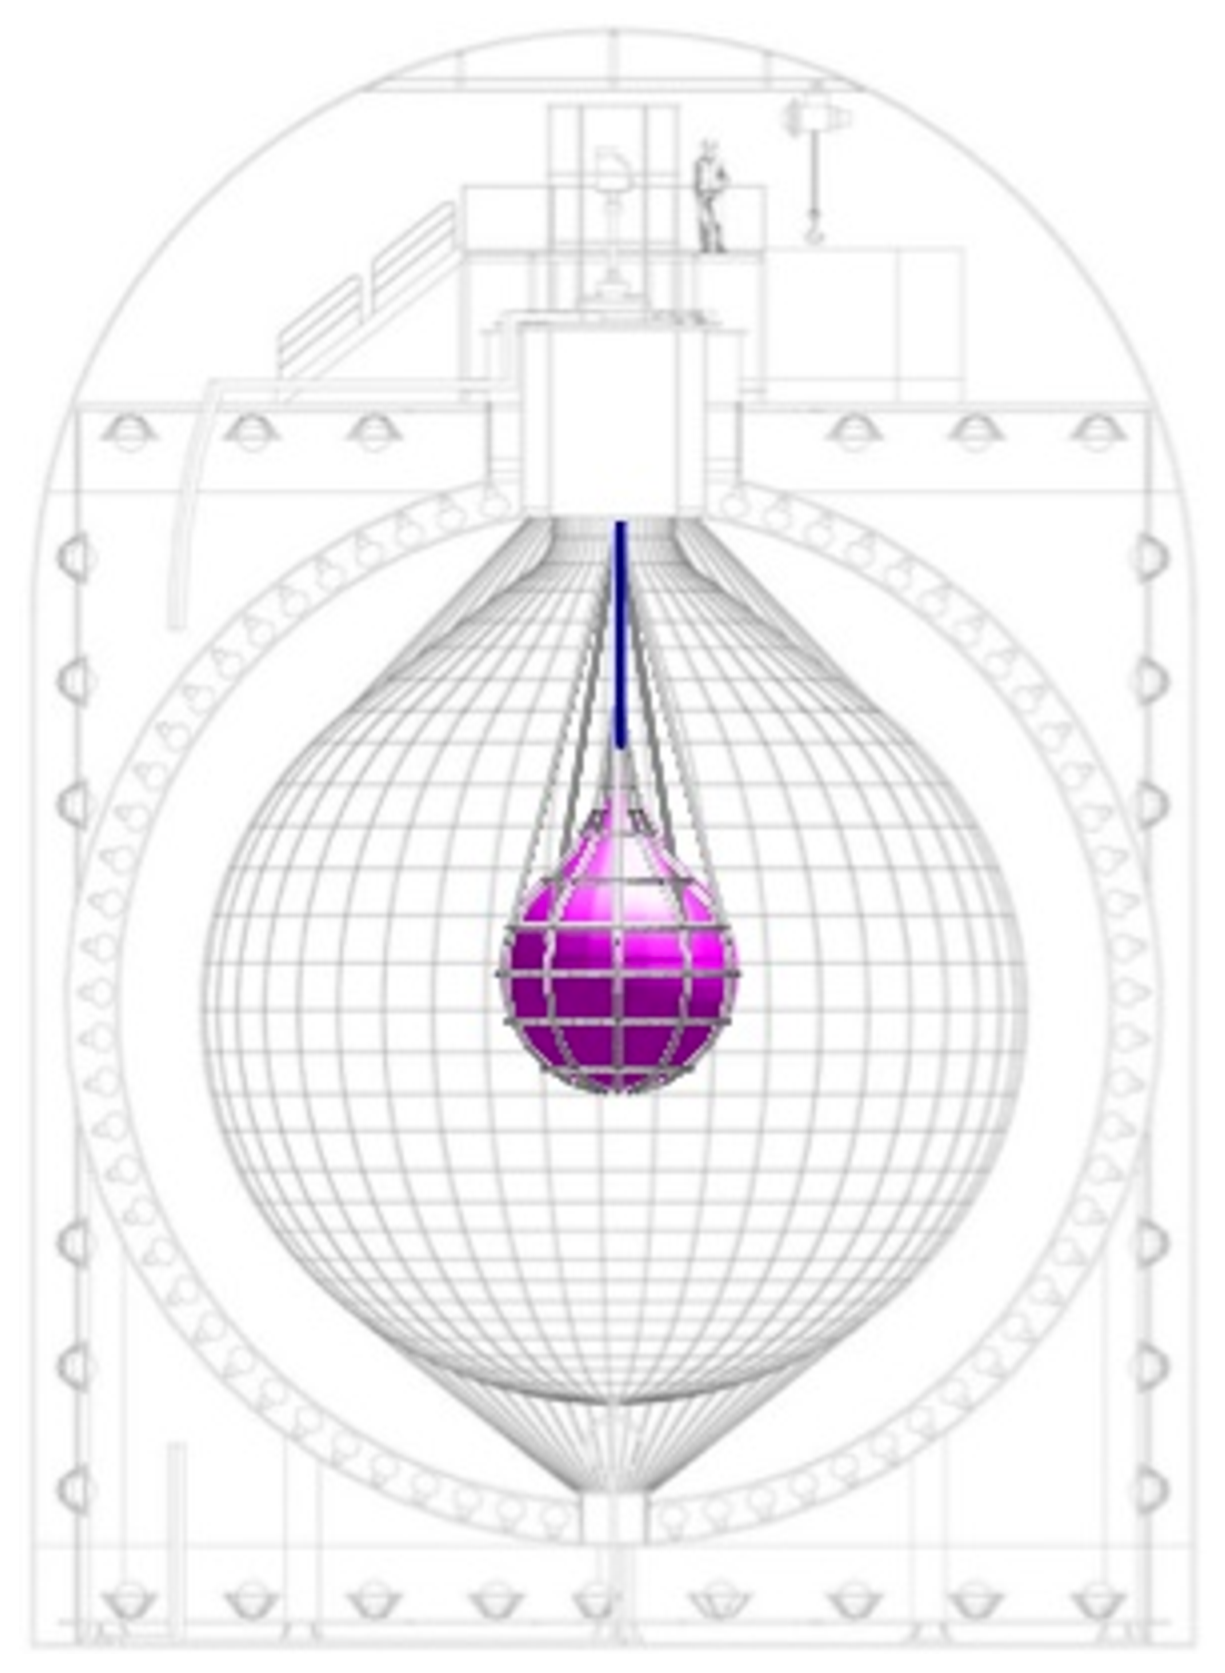
\includegraphics[scale=0.25]{img/kamlandzen.eps}
%\end{center}
%\caption{Sketch of the KamLAND-Zen detector. The ball-on containing the dissolved xenon (purple) hangs in the center of the active volume.} %\label{fig:kamlandzen}
%\end{figure}
%%%%%%

%The KamLAND-Zen experiment plans to dissolve 389 kg of \XE\ in the liquid scintillator of KamLAND in the first phase of the experiment, and up to 1 ton in a projected second phase. 

%The proven resolution (from the previous operation of the KamLAND experiment) is 16\% FWHM at 1 MeV. The main sources of expected background are the \bbtnu\ tail, \BI\ impurities in the scintillator or in the balloon, $^{10}$C generated in the scintillator by cosmic rays, and $^{8}$B solar neutrinos. The expected background rate in the region of interest is $2\times10^{-4}$ \ckky\ \cite{kozlov2011status}, corresponding to $2.2\times10^{-4}$ \ckkbby .

%At the time of writing this report, the mini-balloon installation into the KamLAND detector has been completed, and detector commissioning is ongoing. Physics data-taking with the xenon-loaded liquid scintillator is expected to start in the fall of 2011.



%--------------------------------------------


The KamLAND-Zen experiment is a neutrinoless double beta decay search conducted using the KamLAND detector, a liquid scintillator-based neutrino detector located in the Kamioka mine in Japan. The experiment utilises a large volume of liquid scintillator, doped with a high concentration of Xenon enriched in the Xe136 isotope to enhance the sensitivity to neutrinoless double beta decay.

The KamLAND-Zen detector re-uses the KamLand facility, a spherical volume filled with approximately 1000 tons of liquid scintillator. This volume, designed originally to detect MeV neutrinos, have a very low concentration of $^{238}$U and $^{232}$Th, at the level of 5.0x10$^{-18}$ and 1.3x10$^{-17}$ respectively and it is used in Kamland-Zen as active veto. At the center of this volume, a smaller balloon made out of ethylene-vinylalcohol co-polymer and nylon with a 6.5 m radius and 135 $\mu$m thickness defines a different scintillating volume with xenon dissolve in it. This design allows for accumulation of large amounts of isotope in a very clean environment, the detector configuration also allows to reconstruct the position of the events, allowing to select events far from the ballon walls.
On the other hand as the measurement is based only on the scintillation light, they lack of a good energy resolution producing relatively large background rates in their region of interest when compared with other experiments. In addition, the capabilities of KamLAND-Zen to distinguish among different type of particle interactions is very reduce, although some efforts using neural networks \cite{https://arxiv.org/abs/2203.01870} allow for slightly improved background rejection.
Another issue they face due to their large volume is the relevant contribution to the total background of spallation products that forces to add analysis cuts to select event separated enough in time from muon-induced showers.


%%%%%
\begin{figure}[t!]
\begin{center}
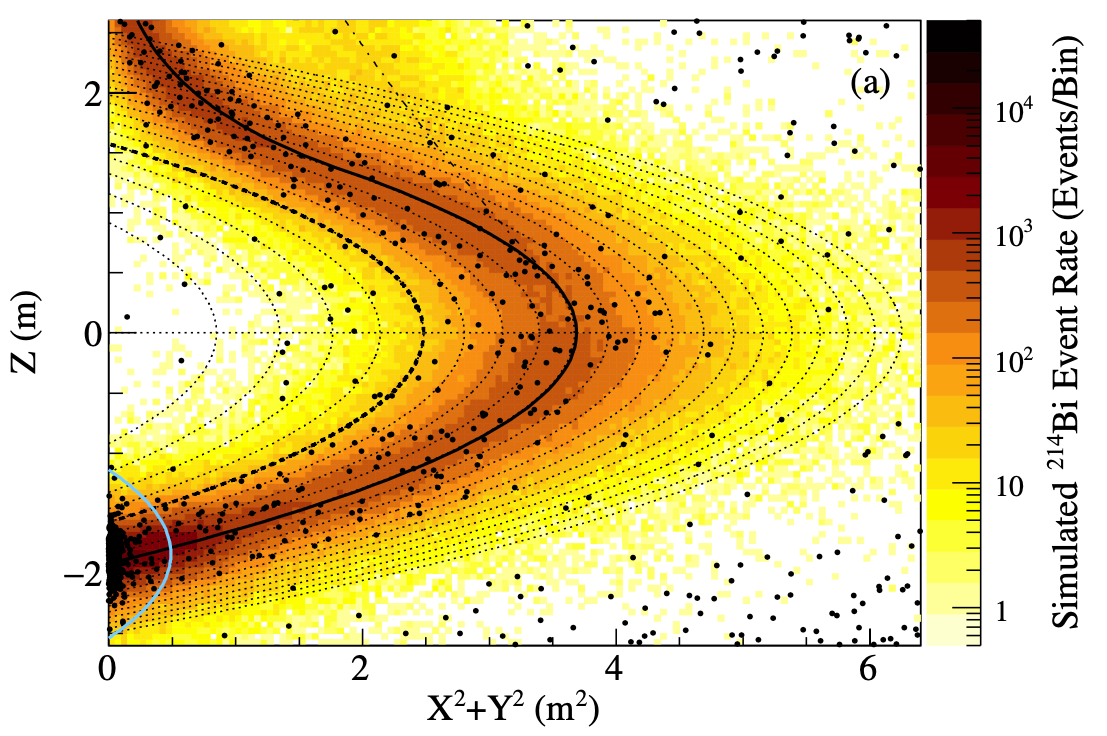
\includegraphics[scale=0.25]{img/KL_fidutial}
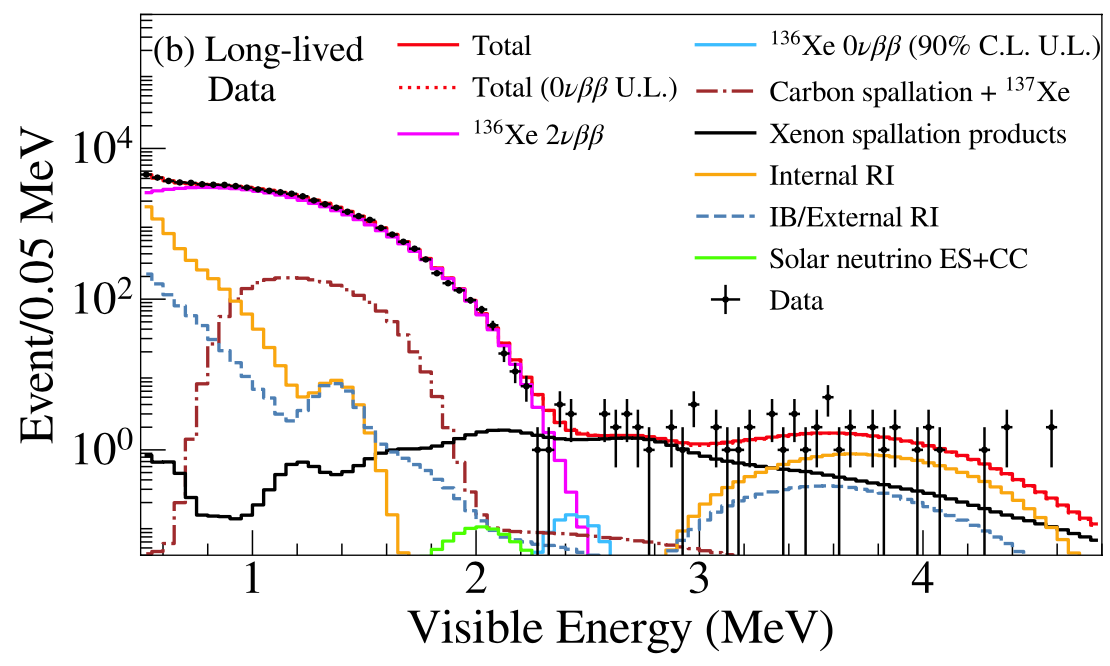
\includegraphics[scale=0.25]{img/KL_LD_events}
\end{center}
\caption{Top:Vertex distribution of candidate events (black points) overlaid on $^{214}$Bi background events from the MC simulation (color histogram) in the energy region 2.35 < E < 2.70 MeV (\bbonu\ window), with arbitrary normalization. The solid and thick dashed lines indicate the shape of the IB and the 1.57-m-radius spherical volume, respectively. The dot-dashed line indicates the nylon belt suspending the inner ballon. The thin dashed lines illustrate the shape of the equal-volume spherical half-shells, which compose the 2.5-m-radius spherical fiducial volume. The high-count region at the IB bottom indicates the hot spot and is vetoed.
Bottom:Energy spectra of selected ββ candidates within a 1.57-m-radius spherical volume drawn together with best-fit backgrounds, the 2νββ decay spectrum, and the 90\% C.L. upper limit for \bbonu\ decay of  long-lived data (LD).
} \label{fig:kamlandzen}
\end{figure}
%%%%%%


The current phase of the KamLAND-Zen experiment uses 745 kg of xenon enriched at the 91\% level in the \XE\ isotope \cite{https://arxiv.org/abs/2203.02139}. This is nearly a factor of two in active mass with respect the previous phase of the experiment. The KL collaboration has recently published the results of their last period of data taking \cite{https://arxiv.org/abs/2203.02139} that corresponds to a total exposure of 970 kg yr of \XE\ . Along this period they observe a total of 24 background events, which can be described by the background-dominated approximation. In this analysis they do not find event excess over the expected background setting a limit to the  half-limit in Xe that corresponds to $T_{1/2} > 2.0X10^{26}$ yr (90\% C.L.), even when their sensitivity was 1.3X10$^{26}$. The combined analysis of this data with the KamLAND-Zen 400 pushes further this limit to $T_{1/2} > 2.3X10^{26}$ yr (90\% C.L.), being the best world limit to this process for xenon.
These results set upper limits on the effective Majorana mass of 36-156 meV depending of the NMEs used.


% \subsection{NEXT} \label{subsec:next}
% The Neutrino Experiment with a Xenon TPC (NEXT) \cite{NEXT:2011eyk} will search for \bbonu\ in \XE\ using a 100-kg high-pressure gaseous xenon (HPXe) time projection chamber. 
Such a detector can provide both good energy resolution and event topological information for background rejection \cite{Nygren:2009zz}.

Double beta decay events leave a distinctive topological signature in HPXe: a ionization track, of about 30 cm long at 10 bar, tortuous due to multiple scattering, and with larger energy depositions at both ends (see fig.~\ref{fig:next_track}). The Gotthard experiment \cite{Luscher:1998sd}, consisting in a small xenon TPC (5.3 kg of xenon, 68\% enrichment in \XE ) operated at 5 bar, proved the effectiveness of such a signature to reject background, achieving a background rate of only $\sim0.01$ \ckky.

%%%%%
\begin{figure}[t!]
\vspace{0.75cm}
\begin{center}
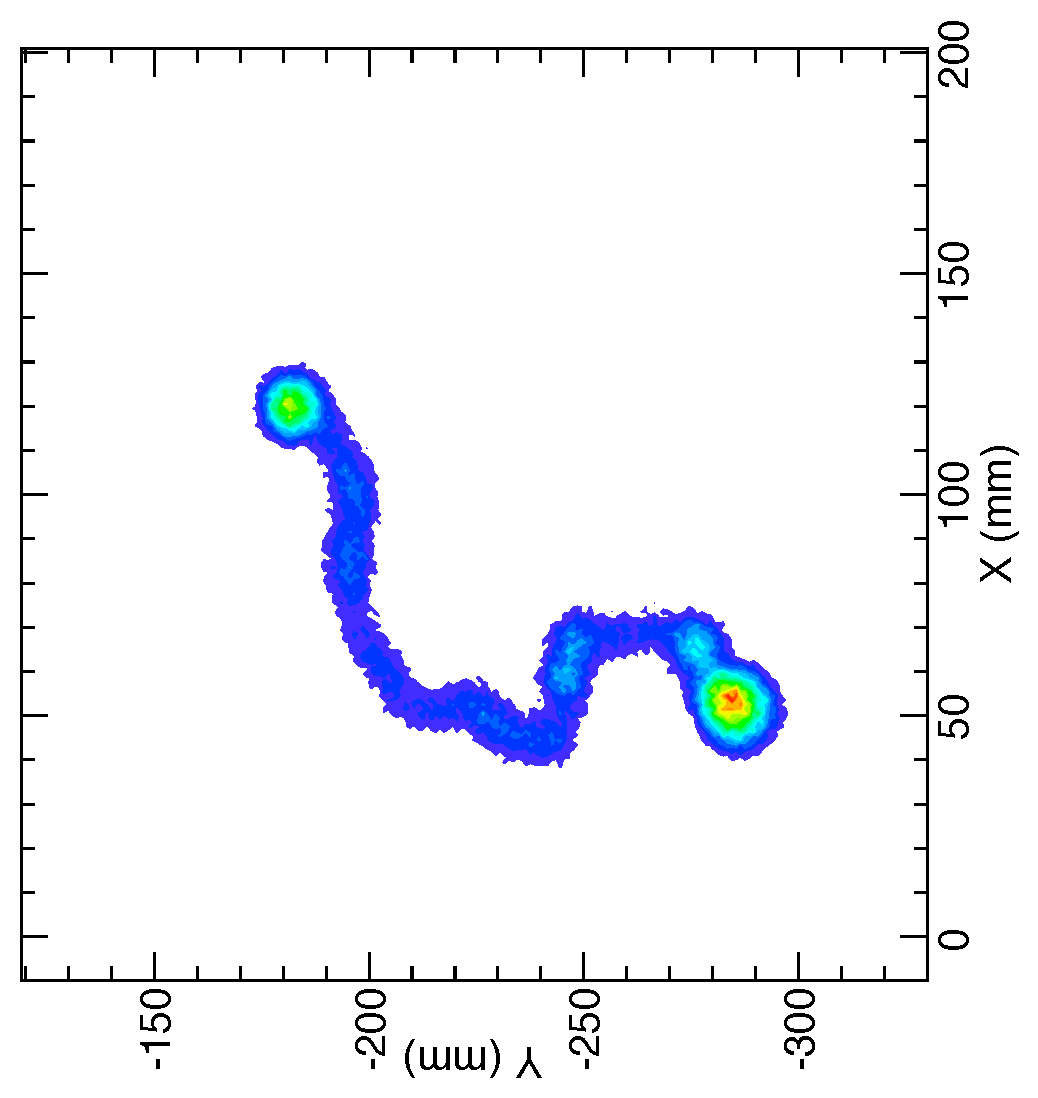
\includegraphics[angle=-90,scale=0.45]{img/bb0nu_track_10atm.eps}
\end{center}
\caption{Simulation of a \bbonu\ track in gaseous xenon at 10 bar \cite{NEXT:2011eyk}.} \label{fig:next_track}
\end{figure}
%%%%%

The design of NEXT is optimized for energy resolution (better than 1\% FWHM at $Q_{\beta \beta}$) by using proportional electroluminescent (EL) amplification of the ionization signal. The detection process is as follows. Particles interacting in the HPXe transfer their energy to the medium through ionization and excitation. The excitation energy is manifested in the prompt emission of VUV ($\sim$178 nm) scintillation light. The ionization tracks (positive ions and free electrons) left behind by the particle are prevented from recombination by a strong electric field (0.5--1.0 kV/cm). Negative charge carriers drift toward the TPC anode, entering a region, defined by two highly-transparent meshes, with an even more intense electric field (3.5 kV/cm/bar). There, further VUV photons are generated isotropically by electroluminescence. Therefore, both scintillation and ionization produce an optical signal, to be detected with a sparse plane of PMTs located behind the cathode. The detection of the primary scintillation light constitutes the start-of-event ($t_0$), whereas the detection of EL light provides an energy measurement. Electroluminescent light provides tracking as well, since it is detected also a few mm away from production at the anode plane, via a dense array (1 cm pitch) of 1-mm$^{2}$ SiPMs.

The NEXT detector will operate at 10 bar, with xenon enriched at 90\% in the \XE\ isotope. At that pressure the 100 kg mass of xenon results in a volume of $\sim$2.5 m$^3$.

The major benefits of the NEXT 100 proposal are its high background rejection factor, resulting in an expected background rate of $2\times 10^{-4}$ \ckkbby , and the fact that xenon is relatively easy (cheap) to enrich and obtain in large quantities.

The NEXT Collaboration expects to commission the detector at the end of 2013. The experiment plans to start its physics run in the second half of 2014.


% \subsection{SNO+} \label{subsec:sno+}
% SNO+ \cite{Kraus:2010zzb} is the follow-up of the successful SNO experiment \cite{SNO:1999crp}, located at SNOLAB, in Canada. It re-uses the existing equipment of the detector (acrylic vessel, photomultipliers and their support structure, electronics and the light water shield) replacing the heavy water by $\sim$780 tonnes of liquid scintillator (linear alkylbenzene, LAB).

The physics program of the SNO+ detector includes measurements of low energy solar neutrinos and \bbonu\ searches using \ND. In order to do that, the liquid scintillator will be loaded with a neodymium salt, resulting in about 50 kg of \ND. This isotope has the second highest endpoint, 3.37 MeV, and the fastest predicted neutrinoless double beta decay rate due to its large phase space factor, see fig.~\ref{fig:g0nu}. The high endpoint is above most radioactive backgrounds, such as radon, and this is a significant advantage. However, enrichment of this isotope seems difficult.

The energy resolution of the SNO+ detector is estimated to be 6.5\% FWHM at 3.4 MeV. External backgrounds can be rejected with a relatively tight fiducial volume selection, cutting however about 50\% of the signal. The most important sources of background are expected to be \TL\ impurities in the scintillator, the irreducible background from $^{8}$B solar neutrinos and \bbtnuº events from \ND . Assuming the radiopurity levels for the liquid scintillator achieved by BOREXINO ($\sim10^{-17}$ g/g of \TL) \cite{Borexino:2009awt}, simulations predict a background rate of $\sim10^{-2}$ \ckkbby\ \cite{Wright:2009csa}. 

The SNO+ experiment is expected to start commissioning in the spring of 2013 with pure liquid scintillator, to be followed by the Nd-loaded liquid scintillator phase. Given that the LAB liquid scintillator is about 15\%  less dense than the surrounding light water, one of the major technical challenges of the SNO+ upgrade is the design of a hold-down system for the acrylic vessel using a net of radiopure ropes, see fig.~\ref{fig:snoplus_anchor_possibility}.  

%%%%%
\begin{figure}[t!b!]
\begin{center}
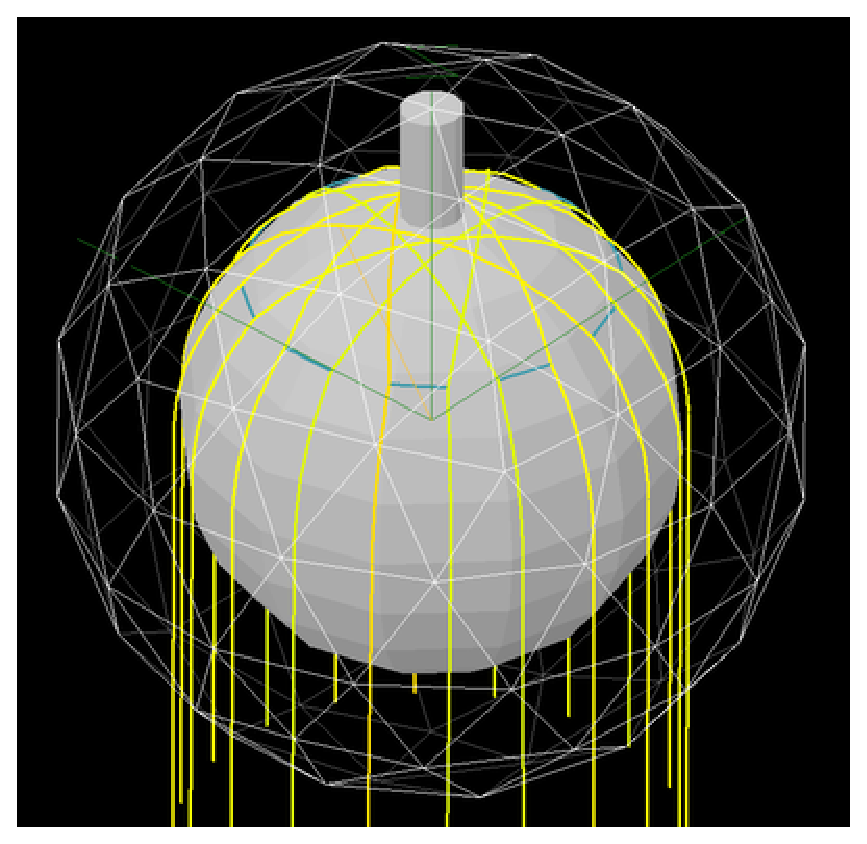
\includegraphics[width=0.55\textwidth]{img/Snoplus_anchor_possibility.eps}
\end{center}
\caption{\label{fig:snoplus_anchor_possibility}One of the candidate configurations for the SNO+ acrylic vessel anchor system. The acrylic vessel is shown in grey, and the anchor system in yellow. The outer sphere made of triangles is the PMT support structure.} 
\end{figure}
%%%%%

% \subsection{SuperNEMO} \label{subsec:snemo}
% This proposed new installment of the NEMO detectors series consists of up to 20 tracker-calo modules, each one containing a thin foil of about 5 kg of \bb-decaying material, probably \SE, although other isotopes such as \ND\ or \CA\ are also under consideration. 

A sketch of a SuperNEMO module can be seen in fig.~\ref{fig:snemo}. The source foil, 3 meters high and 4.5 meters long, with a surface density of about 40 mg/cm$^{2}$, is placed in the center of a tracking chamber with overall dimensions of 4 m height, 5 m length and 1 m width. Nine planes of drift cells operating in Geiger mode and a magnetic field of 25 Gauss allow to reconstruct the trajectory and charge of particles crossing the chamber. A calorimeter consisting of blocks of plastic scintillator coupled to low-activity PMTs surrounds the tracking chamber on four sides. Its granularity allows the energy of individual particles to be measured.

%%%%%
\begin{figure}[t!b!]
\begin{center}
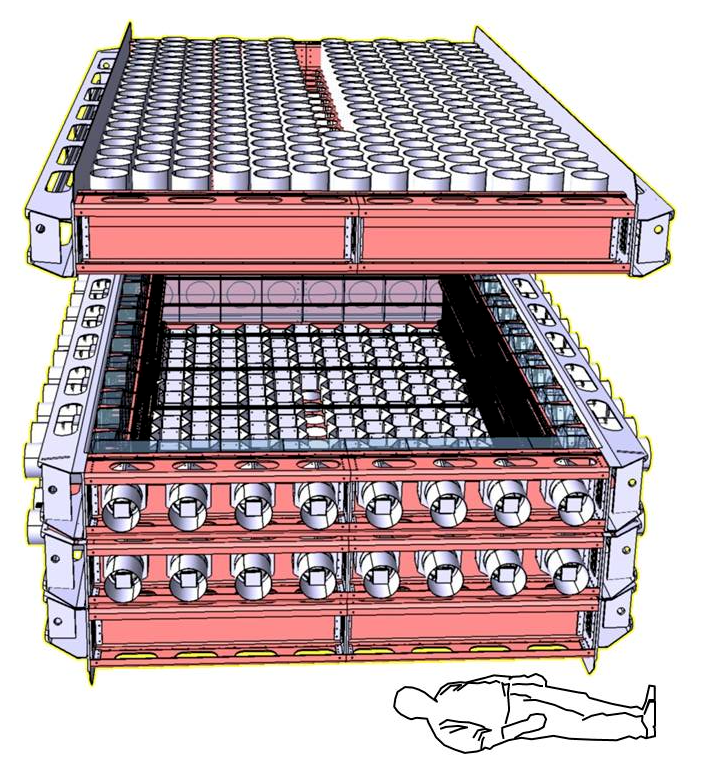
\includegraphics[angle=270,width=0.45\textwidth]{img/snemo-1.eps} \hspace{0.04\textwidth}
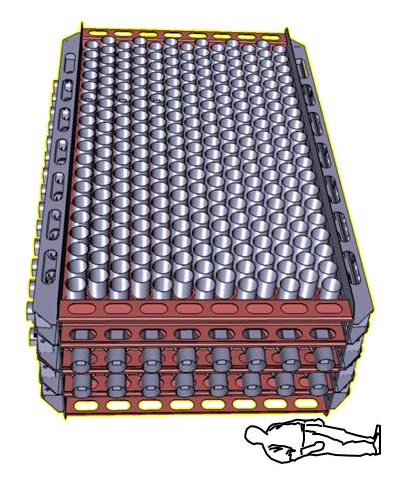
\includegraphics[angle=270,width=0.45\textwidth]{img/snemo-2.eps}
\end{center}
\caption{A SuperNEMO module. The source foil (not shown) is placed in the center of a tracking volume consisting of drift cells operating in Geiger mode. The tracking volume is surrounded by calorimetry consisting of scintillator blocks connected to PMTs (grey). The support frame is shown in red.} \label{fig:snemo}
\end{figure}
%%%%%

The physics case of SuperNEMO relies on several significant improvements over the NEMO-3 detector performance \cite{Shitov:2010nt}. The energy resolution is expected to be 7\% FWHM at 1 MeV, a factor of 2 better than in NEMO-3. Such a resolution has been attained with a 28 cm hexagonal PVT scintillator directly coupled to a 8-inch PMT \cite{Freshville:2011zz}. The detection efficiency of SuperNEMO is estimated by means of simulation to be about 30\%, almost a factor of 2 better than in NEMO-3. As far as the backgrounds are concerned, SuperNEMO goals require an impressive improvement in the purification (both chemical and via distillation methods) of the source foils. In particular, \BI\ and \TL\ contamination in \SE\ foils are to be reduced by factors of 50 and 170, respectively. A dedicated setup, the BiPo detector, installed in the Laboratorio Subterr\'aneo de Canfranc (LSC), will measure the radiopurity of the foils in order to make sure that the required levels are achieved. Finally, in order to decrease radon gas levels in the tracking chamber down to negligible levels ($<$0.15 mBq/m$^3$ ), a reduction of at least a factor of 40 with respect to NEMO-3 is needed. 

The first SuperNEMO module, called the demonstrator, will be the first step from R\&D to construction with the aims to demonstrate the feasibility of large scale mass production, to measure the backgrounds (especially from radon emanation), and to finalize the detector design. The demonstrator will be installed in the space previously occupied by the NEMO-3 detector at the Modane Underground Laboratory.

The current plans of the SuperNEMO Collaboration for the following: (a) demonstrator construction, 2010--2012; (b) demonstrator physics run start-up, 2013; and (c) full detector construction start-up, 2014. 

% \subsection{Other proposals} \label{subsec:other}
% \subsubsection*{CANDLES} This project \cite{Umehara:2010zz} proposes the use of CaF$_{2}$ scintillating crystals to search for \bbonu\ in \CA. The crystals would be immersed in liquid scintillator providing shielding and an active veto against external backgrounds. Among the \bb\ isotopes, \CA\ has the highest $Q$-value, 4.27 MeV. This places the signal well above the energy region of the natural radioactive processes. Unfortunately, the natural abundance of the isotope is only 0.187\% and enrichment seems complicated. Therefore, many tons of crystals are needed for a competitive new-generation experiment.  
%
\subsubsection*{COBRA} The COBRA experiment \cite{Zuber:2001vm, Zuber:2010zz} is exploring the potentials of Cadmium Zinc Telluride (CdZnTe) room-temperature semiconductor detectors for \bbonu\ searches. Out of the several \bb\ candidate isotopes in CdZnTe, COBRA is focusing on \TE, because of its natural abundance, and \CD, because of its high $Q$-value of 2.8 MeV. Activities are split in two main directions: (a) the identification of the main background components in a setup of 64 commercial 1-cm$^{3}$ CdZnTe diodes located at LNGS; and (b) the development of pixelized devices that would allow to reduce the background by particle identification.
%
\subsubsection*{DCBA} The Drift Chamber Beta-ray Analyzer \cite{Ishikawa:2011zza} is a magnetized tracker (drift chambers) that can reconstruct the trajectories of charged particles emitted from a \bb\ source foil. The momentum and kinetic energy are derived from the track curvature in the magnetic field. A prototype, DCBA-T2, has shown energy resolution of about 150 keV (FWHM) at 1 MeV, and the main source of background (\BI) has been identified. A new apparatus, DCBA-T3, with a more intense magnetic field is now under construction at KEK.
%
\subsubsection*{LUCIFER} The idea of LUCIFER \cite{Giuliani:2010zz, Ferroni:2011zz} is to join the bolometric technique proposed for the CUORE experiment with the bolometric light detection technique used in cryogenic dark matter experiments. Preliminary tests on several \bbonu\ detectors have clearly demonstrated the background rejection capabilities that arise from the simultaneous, independent, double readout (heat and scintillation). LUCIFER will consist of an array of ZnSe crystals operated at 20 mK. The proof of principle with about 10 kg of enriched Se is foreseen for 2014.
%
\subsubsection*{MOON} The MOON detector \cite{Ejiri:2010zz} is a stack of multi-layer modules, each one consisting of a scintillator plate for measuring energy and time, two thin detector layers for position and particle identification, and a thin \bb\ source film interleaved between them. At present, NaI(Tl) scintillators are considered as the candidates for the scintillator plates. Energy resolution around 3\% FWHM at 3 MeV has been achieved during the R\&D phase. For position-sensitive detectors, possible candidates are multi-wire proportional chambers (MWPCs) and Si-strip detectors. 
%
\subsubsection*{XMASS} XMASS \cite{Sekiya:2010bf, Takeda:2011zza} is a multi-purpose liquid xenon scintillator. Although optimized for dark matter searches, it will also investigate neutrinoless double beta decay and solar neutrinos. The detector, with about 800 kg of xenon, was installed in the Kamioka mine (Japan) in the fall of 2010. The excellent self-shielding capabilities of the liquid xenon will be used to define a virtually background-free inner volume. 
%%%

% \subsection{Sensitivity of new-generation experiments} \label{subsec:sensi}
% In this section we try to assess the physics case of the new-generation double beta experiments described above\footnote{For the sensitivity computation, we restrict ourselves to experiments that involve at least a few kg of \bb\ emitter mass, that are approved, and that have been granted a significant financial support.}. We quote the experimental sensitivities to \mbb, assuming the standard light Majorana neutrino exchange as the dominant \bbonu\ mechanism. To perform this risky exercise we make use of the physics-motivated ranges for the NME values described in sect.~\ref{subsec:nme_pmr}, and of the set of experimental parameters summarized in table~\ref{tab:parameters}. A discussion motivating our choice of parameters in table~\ref{tab:parameters} is given in sect.~\ref{subsec:sensi_assumptions}.

%%%%%
\clearpage
\begin{sidewaystable}[H]
\caption{Basic parameters for the different double beta experiments: \bb\ emitter mass \Mbb, \bbonu\ efficiency $\varepsilon$, FWHM energy resolution $\Delta E$, and background rate $c$ per unit energy, \bb\ isotope mass and time. The last column indicates the number of background events within the ROI, and is the product of the \Mbb, $\Delta E$ and $c$ columns. Comparison of different approaches is very difficult directly from the numbers in the table, but this information is fundamental to compute their sensitivity.}\label{tab:parameters}
\begin{center}
\begin{tabular}{lcccccc}
\hline
Experiment  & \Mbb    & $\varepsilon$ & $\Delta E$ & $c$                  & Bgr/ROI   \\
            & (\kgbb) &               & (keV)      &  ($10^{-3}$ \ckkbby)  & (cts/yr)   \\ \hline
EXO-200     & 141     & 0.34 	      & 100        & 0.78--5              & 11--71  \\
GERDA-1     & 15.2    & 0.95          & 4.2        & 12--70               & 0.77--4.5  \\
GERDA-2     & 30.4    & 0.84          & 2          & 1.2--7               & 0.07--0.43 \\ 
CUORE-0     & 10.9    & 0.83          & 5          & 180--390             & 9.8--21.3  \\
CUORE 	    & 206     & 0.83          & 5    	   & 36--130              & 37.1--134  \\
KamLAND-Zen & 357     & 0.61          & 250 	   & 0.22--1.8            & 19.6--161  \\
MAJORANA Demonstrator   & 17.2    & 0.85          & 2          & 1.2--12              & 0.04--0.41  \\  
SNO+        & 44      & 0.50          & 220        & 9--70                & 87--680 \\
NEXT 	    & 89.2    & 0.33 	      & 18         & 0.2--1               & 0.32--1.6 \\
SuperNEMO Demonstrator  & 7       & 0.28          & 130        & 0.6--6               & 0.55--5.5 \\
 \hline
\end{tabular}
\end{center}
\end{sidewaystable}
%%%%%

Although different experimental aspects are relevant from the point of view of the feasibility of an experiment, the sensitivity can be computed using only a few parameters ---namely, effective mass of the isotope and background rate in the energy Region Of Interest (ROI)--- that can be extracted from the fundamental numbers in the design of the experiments. 

The sensitivity is calculated based on the Feldman-Cousins method \cite{Feldman:1997qc} for constructing confidence intervals, following the prescription given in \cite{Gomez-Cadenas:2010zcc}. For each experiment, we define a ROI centered at the \bb\ decay $Q$-value and extending for one FWHM of energy resolution, and we compute the experimental sensitivity at 90\% confidence level. We take into account the effect of the FWHM selection (corresponding to 76\% efficiency assuming gaussian resolution) as a multiplicative factor to the experimental efficiency reported in table~\ref{tab:parameters}.

 Our prescription assumes a counting experiment in the ROI with a perfectly known background rate. In other words, in our sensitivity computation, we neglect systematic uncertainties\footnote{With one exception for the SNO+ and KamLAND-Zen experiments, see sect.~\ref{subsec:sensi_assumptions}, where an attempt has been made to account for systematic effects affecting energy reconstruction.} and any energy shape information that may be present in the energy distribution of events. Systematic uncertainties may possibly affect the parameters listed above, especially the knowledge of the backgrounds, and deteriorate the sensitivity. On the other hand, use of additional information beyond the overall count rate of \bbonu\ candidates within the ROI may yield some sensitivity improvement. While important, both effects would be extremely difficult to incorporate in such a sensitivity comparison, given that most new-generation experiments discussed here have not even started their commissioning phase, yet.

In fig.~\ref{fig:sens-pmr} we show the \mbb\ sensitivities at 90\% CL for the new-generation proposals discussed above, assuming a 5 years exposure for all of them. The colored rectangles reflect the uncertainty coming from the PMR nuclear matrix elements, see fig.~\ref{fig:nme}. For each experiment, two rectangles are shown, corresponding to the most optimistic and most pessimistic background rate expectations given in tab.~\ref{tab:parameters}, respectively. For most experiments, the two rectangles overlap. For each experiment, the thin solid line at the lowest \mbb\ values is meant to give an idea of what can be gained by increased exposures. The line represents the \mbb\ sensitivity for the most optimistic NME values (within the PMR range of fig.~\ref{fig:nme}) and for the most optimistic background rate expectations (within the ranges of tab.~\ref{tab:parameters}) for a 10 years exposure. For reference, we also show the mass range of the standing KK claim of evidence for \bbonu\ in \GE\ \cite{Klapdor-Kleingrothaus:2006zcr} (with a central value of 300 meV) and the mass region as predicted under the inverted hierarchy hypothesis (between 17 and 52 meV, see fig.~\ref{fig:mbetabetavsmlight}). The sensitivity of the various proposals after a 5 years exposure, both in terms of \Tonu\ and \mbb, is also shown in tab.~\ref{tab:sensitivity}, where the central value of the PMR interval for the nuclear matrix elements and the optimistic background rate expectations in tab.~\ref{tab:parameters} have been assumed.


\begin{figure}[ht]
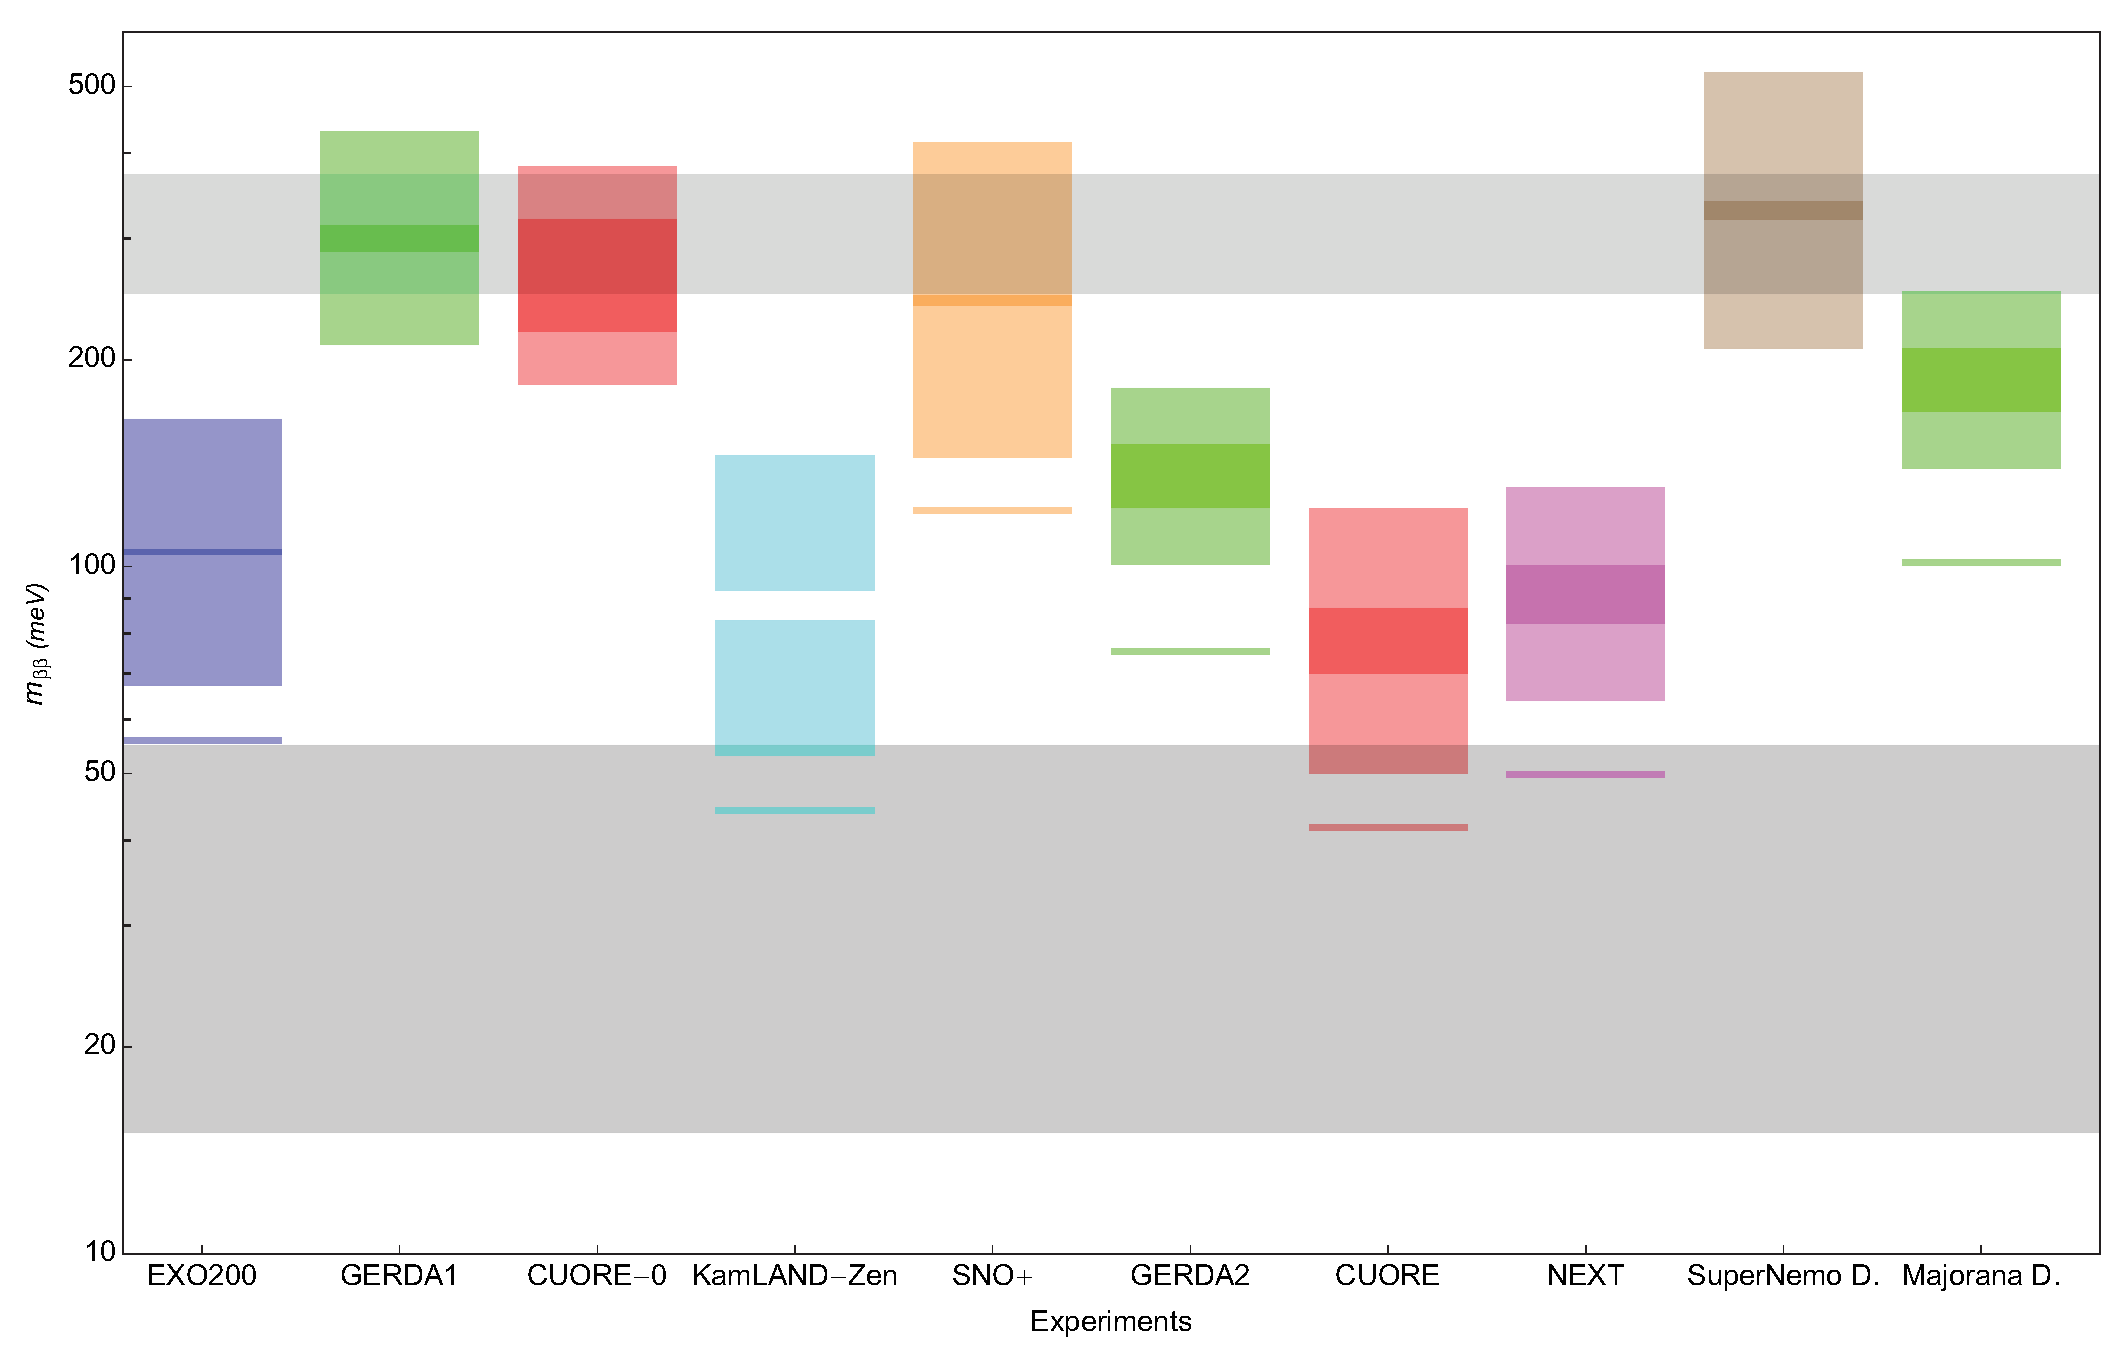
\includegraphics[width=\textwidth]{img/DB_parameters.eps}
\caption{Sensitivity of the different experiments to the neutrino effective mass \mbb\ computed assuming a 5 years exposure, the PMR intervals for the nuclear matrix elements (see sect.~\ref{subsec:nme_pmr}), and for both the optimistic and pessimistic experimental parameters of table~\ref{tab:parameters}. A statistical 90\% CL is computed according to the Feldman-Cousins method \cite{Feldman:1997qc}, assuming a signal region of one FWHM and the corresponding efficiency. For each experiment, the sensitivities for the two experimental parameter sets are drawn as overlapping rectangles. A sensitivity line corresponding to a 10 years exposure, and to the most optimistic NME and experimental parameter set, is also shown. The upper grey region represents the KK claim \cite{Klapdor-Kleingrothaus:2006zcr} while the lower grey region represents the inverted hierarchy region (see fig.~\ref{fig:mbetabetavsmlight}).}
\label{fig:sens-pmr}
\end{figure}


%%%%%
\begin{table}[t!b!]
\caption{Sensitivity of the experiments at 90\% CL after a 5 years exposure, both in terms of half-life \Tonu\ and in terms of neutrino effective mass \mbb . These values are obtained from the optimistic background rate assumptions in tab.~\ref{tab:parameters}. The conversion from \Tonu\ to \mbb\ assumes the central value of the PMR interval for the nuclear matrix elements.}\label{tab:sensitivity}
\begin{center}
%\begin{narrowtabular}{3cm}{lcr}
\begin{tabular}{lcr}
\hline
Experiment & \Tonu\ (years) & \mbb\ (meV) \\ \hline
CUORE-0 	& $8.67\times 10^{24}$ & 203 \\
CUORE 		& $8.86\times 10^{25}$ & 63\\
GERDA-1 	& $4.49\times 10^{25}$ & 252\\
GERDA-2 	& $1.37\times 10^{26}$ & 121\\
EXO200 		& $8.20\times 10^{25}$ & 82\\
NEXT 		& $9.13\times 10^{25}$ & 78\\
KamLAND-Zen 	& $1.32\times 10^{26}$ & 65\\
SNO+ 		& $5.38\times 10^{24}$ & 182\\
SuperNEMO Demonstrator 	& $9.15\times 10^{25}$ & 258\\
MAJORANA Demonstrator	& $7.19\times 10^{25}$ & 258\\
 \hline
%\end{narrowtabular}
\end{tabular}
\end{center}
\end{table}
%%%%%

The first thing to remark from fig.~\ref{fig:sens-pmr} is that the KK claim should be unambiguously solved by several new-generation proposals using different isotopes. If our assumptions are correct, this will certainly be the case for \GE\ (GERDA, MAJORANA), \TE\ (CUORE) and \XE\ (EXO-200, KamLAND-Zen, NEXT), and possibly also for \SE\ (SuperNEMO) and \ND\ (SNO+). Multi-isotope determination of \bbonu\ may therefore become a real possibility within this decade. In this respect, it is important to note that GERDA and MAJORANA are the only experiments among those in fig.~\ref{fig:sens-pmr} using the same isotope of the HM experiment\footnote{Not only: we have seen that GERDA in its first phase re-uses the same detectors as in the HM experiment.}, and should therefore be able to provide the only truly model-independent confirmations of this claim.

On the other hand, several experiments appear to have a very good chance to reach a sensitivity of 100 meV or better, in particular CUORE, KamLAND-Zen, NEXT and EXO-200. In our most optimistic scenario concerning NME values and experimental performances, this target may also be reached by GERDA during its second phase. Given our uncertainties, we cannot predict which, among these 4--5 different experimental proposals, will provide the best \mbb\ sensitivity after a 5 years exposure. To this end, a better knowledge of the actual (as opposed to expected) values for the background rates, of the systematic uncertainties affecting the measurement, and of the NME values would be necessary for all experiments.

From fig.~\ref{fig:sens-pmr}, our expectation is that it will be almost impossible for the new-generation experiments discussed here to discover \bbonu\ after 5 years of exposure if the neutrino mass spectrum is hierarchical ($m_{\rm light}\simeq 0$) rather than degenerate, since essentially no overlap exists between the experimental sensitivities and the 17--52 meV inverted hierarchy region. Not only larger exposures, but also new (better) experimental proposals, would be needed to fully probe this mass region. As mentioned above, we expect experiments using \XE\ (EXO-200, KamLAND-Zen, NEXT) to provide for the first time during this decade a comparable or better sensitivity than \GE\ (GERDA, MAJORANA) and \TE\ (CUORE) experiments, which dominated the field over the past two decades. In perspective, if the low-background expectations of new-generation \XE\ proposals will be confirmed during this decade, \XE\ would be a particularly favorable isotope to use also in the longer term. This is because scalability to isotope masses in the 1-10 ton range are in this case more realistic than with any other isotope. 

\begin{figure}[ht]
\includegraphics[width=\textwidth]{img/DB_models.eps}
\caption{Sensitivity of the different experiments to the neutrino effective mass \mbb\ computed assuming the optimistic experimental parameters of table~\ref{tab:parameters}. A statistical 90\% CL is computed according to the Feldman-Cousins method \cite{Feldman:1997qc}, assuming a signal region of one FWHM and the corresponding efficiency. Five different frameworks for NME calculations are considered, following reference \cite{Dueck:2011hu}, and are drawn as overlapping rectangles. The upper grey region represents the KK claim \cite{Klapdor-Kleingrothaus:2006zcr} while the lower grey region represents the inverted hierarchy region (see fig.~\ref{fig:mbetabetavsmlight}).}
\label{fig:sens-models}
\end{figure}

Figure~\ref{fig:sens-pmr} represents our main result for the physics case comparison of new-generation \bbonu\ experiments. In this figure, a single, physics-motivated, NME uncertainty band is used for each isotope, following our discussion in sect.~\ref{subsec:nme_pmr}. For completeness, we have also repeated the same exercise for several other NME values or ranges, one for each theoretical framework considered in \cite{Dueck:2011hu}. The result is shown in fig.~\ref{fig:sens-models}. As mentioned above, the spread of the corresponding \mbb\ predictions most likely overestimates the theoretical uncertainty in the \Tonu\ $\to$ \mbb\ sensitivity conversion. For figure clarity, only nuclear theory assumptions are varied in fig.~\ref{fig:sens-models}, while the detector performance parameters are fixed to the most optimistic values of tab.~\ref{tab:parameters}. As can be seen in fig.~\ref{fig:sens-pmr}, our assumed uncertainties in the detector performance parameters would yield \mbb\ sensitivity changes of about the same size as the nuclear theory variations shown in fig.~\ref{fig:sens-models}.


% \subsection{Validity of sensitivity assumptions} \label{subsec:sensi_assumptions}
% The reliability of the sensitivity estimates given above critically depend on how realistic our choice of detector performance indicators is. In this section, we discuss how we have chosen the parameters reported in tab.~\ref{tab:parameters}. This discussion is mostly intended for the expert reader wishing to independently assess our choices, and to use his/her own judgment to modify them accordingly. Given that the largest uncertainty affecting the ultimate \mbb\ sensitivity of a proposal is almost always related the achievable background rates, we decide to quote a background rate range. For all other indicators, a single number rather than a range is used, see tab.~\ref{tab:parameters} 

The EXO-200 TPC is filled with about 175 kg of liquid xenon enriched to 80.6\% in the isotope \XE\ \cite{EXO-200:2011xzf}, corresponding to a \bb\ mass of about 141 \kgbb. For the \bbonu\ efficiency around \Qbb, we take the efficiency assumed by the EXO Collaboration for their \bbtnu\ analysis \cite{EXO-200:2011xzf}, corresponding to $\varepsilon = 0.34$ above the 720 keV analysis threshold. The inefficiencies are dominated by the fiducial volume cut, keeping 63 out of 175 kg of liquid xenon \cite{EXO-200:2011xzf} (0.36 efficiency). A 6.3\% inefficiency introduced by vetoing $\beta$-$\alpha$ coincidences \cite{EXO-200:2011xzf} has also been considered in our efficiency assumption. In \cite{EXO-200:2011xzf}, the collaboration measured an energy resolution of $\sigma_E/E=4.5\%$ at 2615 keV for the EXO-200 detector. This value was obtained using a 376 V/cm drift field and ionization signals only. An improvement of up to a factor of 2.5 could be achieved with higher (1--4 kV/cm) drift fields and combining ionization with scintillation information, see \cite{EXO-200:2003bso}. As a result, we assume a nearly-nominal, 4.2\% FWHM energy resolution at \Qbb, corresponding to about 100 keV. For our background rate lower limit, we consider the collaboration's goal of 20 radioactive background events per year in a $\pm 2\sigma$ interval around the \Qbb\ endpoint, for a $\sigma/E=1.6\%$ energy resolution at 2.5 MeV, a detector mass of 200 kg and a 80\% enrichment in \XE\ \cite{Hall:2010zzg}. From these numbers, we obtain a background rate of $c=0.78\times 10^{-3}$ \ckkbby. This nominal background rate prediction still remains to be updated based on real EXO-200 data. As a worst-case background rate scenario, we take the rate that has already been achieved: $4\times 10^{-3}$ \ckky, see \cite{EXO-200:2011xzf}. This background level was obtained without full lead shielding, radon exclusion tent, radon trap or full 3-dim reconstruction, and might therefore be improved in the future \cite{EXO-200:2011xzf}. This number corresponds to $c=5\times 10^{-3}$ \ckkbby\ per unit \bb\ mass.

GERDA-1 will use eight refurbished \GE\ diodes from the Heidelberg-Moscow and IGEX experiments, for a total active mass of 17.66 kg and 0.86 isotopic enrichment in \GE\ \cite{Knopfle:2012zz}, corresponding to a \bb\ mass of 15.2 \kgbb. As for the \bbonu\ efficiency, the actual value will ultimately depend on analysis details that are unknown at the moment, for example whether the collaboration will rely on pulse shape discrimination already in phase I to further reduce multi-site energy deposition events. In the absence of an updated number, we assume $\varepsilon =0.95$ as originally quoted by the collaboration in \cite{Abt:2004yk}. The FWHM energy resolution for GERDA-1 diodes was measured to be between 3.6 and 6.0 keV at the 2615 keV gamma ray line from \TL\ \cite{Cattadori:2012fy}. Taking the central value of this interval (4.8 keV) and extrapolating to the \GE\ \Qbb\ value (2.039 MeV), we estimate $\Delta E= 4.2\ \text{keV}$. The optimistic background rate scenario is assumed to be the collaboration's goal of 0.01 \ckky\ \cite{Abt:2004yk}, corresponding to 0.012 \ckkbby\ per unit \bb\ mass. GERDA started commissioning in mid-2010, and data obtained since then can be used to estimate a worst-case scenario for the achievable background rates. The best background rate measured with a string of 3 natural germanium detectors, refurbished from the Genius-TF experiment, is $0.06\pm 0.02$ \ckky\ \cite{Cattadori:2012fy}. Since mid-2011, the first enriched germanium detectors have been deployed on a second string arm, using the best detector configuration found so far. Preliminary data from the enriched germanium detectors indicate a background rate that is compatible with the one found with the natural germanium diodes \cite{Cattadori:2012fy}. As a consequence, we assume 0.06 \ckky\ as upper limit for the GERDA-1 background rate, translating into $c=0.07$ \ckkbby\ per unit \bb\ mass.

For the phase II of the experiment, the GERDA Collaboration purchased 37.5 kg of germanium with an isotopic abundance in \GE\ of 0.86. The material has already been purified into 35.4 kg of 6N germanium, corresponding to a \bb\ mass of 30.4 \kgbb. In order to reduce backgrounds, both sophisticated pulse-shape discrimination (PSD) techniques and additional instrumentation for the LAr veto are likely to be used by GERDA-2. We assume an overall \bbonu\ efficiency of $\varepsilon =0.84$, given by the product of the 0.86 efficiency for a PSD cut reported in \cite{Agostini:2010rd}, times the 0.973 efficiency for a LAr veto cut reported in \cite{heisel2011large}. Compared to phase I detectors, a significantly improved FWHM energy resolution of 2 keV at \Qbb\ has been measured for the BEGe detectors to be used by GERDA-2, see \cite{Agostini:2010ke}. The lower limit on the background rate is taken to be the collaboration's goal of 0.001 \ckky\ \cite{Abt:2004yk}, corresponding to $c=0.0012$ \ckkbby. Again, we use preliminary results from the GERDA commissioning runs to estimate an upper limit on the background rate. Commissioning data indicate that $\beta$ decays of $^{42}$K, that is in turn produced positively charged by the $^{42}$Ar decay within the LAr veto, can contribute very significantly to the \Qbb\ background rate. This $^{42}$K background can be most easily quantified by measuring the 1525 keV gamma ray line. On the one hand, the collaboration estimated via simulations that a background rate at \Qbb\ of up to $1.7\times 10^{-3}$ \ckky\ can be obtained by a homogeneous distribution of $^{42}$K around the detectors, for a 43.9 $\mu\text{Bq/kg}$ contamination in $^{42}$K \cite{lehnert2011analysis}. On the other hand, a 1525 keV line about 20 times more intense than expected was observed during the first commissioning run. A significant fraction of this enhancement has been understood as due to a inhomogeneous $^{42}$K distribution caused by the field lines drifting the positively-charged $^{42}$K ions to the detector surface. To prevent the $^{42}$K ions to reach the detector surfaces, the collaboration deployed a copper shield called the \emph{``mini-shroud''}. The additional shroud reduced the counts at the 1525 keV line and at \Qbb\ by a factor of 4-5, and a preliminary measurement of the $^{42}$Ar specific activity of about 160 $\mu\text{Bq/kg}$ was obtained for almost field-free runs \cite{Knopfle:2012zz}. This measured value, combined with the simulation result of $1.7\times 10^{-3}$ \ckky\ for a 43.9 $\mu\text{Bq/kg}$ contamination in $^{42}$K, motivates our upper limit background rate assumption of about 0.006 \ckky, or $c=0.007$ \ckkbby\ per unit \bb\ mass.

CUORE-0 will make use of a single CUORE-like tower with 39 kg of natural TeO$_2$ crystals and with an isotopic abundance of 0.34167 of \TE\ \cite{CUORE:2011boi}, corresponding to a \bb\ mass of 10.9 \kgbb. The overall signal efficiency has been estimated to be about $0.83$, as obtained for the big crystals of the CUORICINO experiment \cite{Andreotti:2010vj}. The main inefficiency source is the ``physical'' inefficiency due to beta particles escaping the detector and radiative processes. The expected FWHM energy resolution of the CUORE detectors is $\Delta E\simeq 5\ \text{keV}$ at the \bbonu\ transition energy \cite{CUORE:2011boi}. As lower limit on the background rate, we assume 0.05 \ckky\ from the 2.615 keV gamma ray multi-Compton events coming from the irreducible \THORIUM\ contamination of the CUORICINO cryostat, as done in \cite{CUORE:2011boi}. This rate corresponds to $c=0.18$ \ckkbby\ per unit \bb\ mass. As upper limit on the background rate, again we follow \cite{CUORE:2011boi} and assume 0.11 \ckky, translating into $c=0.39$ \ckkbby\ per unit \bb\ mass. This latter number includes an additional background contribution from scaling the CUORICINO background in the conservative case of a factor of 2 improvement in \URANIUM\ and \THORIUM\ contamination of the copper and crystal surfaces. Such surface contamination results in degraded alphas that may mimic the \bb\ signal. This factor of 2 improvement is largely motivated by the background rates measured in the Three Towers Test (TTT), allowing to estimate the surface contamination of the copper detector holders, responsible for a large ($50\pm 20\%$ \cite{CUORE:2011boi}) fraction of the CUORICINO backgrounds \cite{Alessandria:2011vj}. For such tests, crystals were dismounted from the CUORICINO detector, and repolished on the surfaces. Three different types of copper cleaning were tested. The copper treatment procedure selected by the collaboration proved to be able to reduce the copper surface contamination by at least a factor of 2 compared to CUORICINO \cite{CUORE:2011boi,Alessandria:2011vj}.  

The CUORE total active mass will be 741 kg for the 988 envisaged cubic detectors \cite{CUORE:2011boi}. As for CUORE-0, the natural TeO$_2$ crystals will have an isotopic abundance of 0.34167 of \TE\ \cite{CUORE:2011boi}, resulting in about 206 \kgbb\ of \TE. The overall signal efficiency and the FWHM energy resolution at \Qbb\ are assumed to be equal to the CUORE-0 figures given above, $\varepsilon =0.83$ and $\Delta E\simeq 5\ \text{keV}$, respectively. The main improvements in background rate reduction compared to CUORE-0 are assumed to come from a much cleaner cryostat and from the different detector geometry. Under these assumptions, the CUORE background will be dominated by copper and crystal surface contaminations. As lower limit on the background rate, the 0.01 \ckky\ goal of the collaboration is assumed \cite{CUORE:2011boi,CUORE:2003fpg}, corresponding to $c=0.036$ \ckkbby. As upper limit, an extrapolation of the currently available measurements \cite{Alessandria:2011vj} on copper and crystal surface contaminations to the CUORE geometry results in a 0.035 \ckky\ upper limit \cite{Gorla:2012gd}, resulting into $c=0.13$ \ckkbby\ per unit \bb\ mass.  

During the phase I of the experiment, KamLAND-Zen will use 389 kg of xenon \cite{kozlov2011status}, enriched to 0.917 \cite{koga2010kamland} in the isotope \XE, for a \XE\ total mass of 357 \kgbb. Concerning \bbonu\ efficiency, the collaboration will make use of a fiducial volume cut to suppress backgrounds that are external to the mini-balloon, for example due to \URANIUM/\THORIUM\ contaminations in the outer liquid scintillator or the environmental gamma ray background. Depending on the \URANIUM/\THORIUM\ contamination levels of the mini-balloon materials themselves (Nylon film, supporting ropes and pipes), the collaboration is also considering a tighter fiducial volume cut to suppress backgrounds originating from the mini-balloon. In the following, we assume that a fiducial volume definition placed 3~$\sigma_r$ inward with respect to the mini-balloon surface will be used, where $\sigma_r$ is the radial position reconstruction accuracy. Assuming $\sigma_r=\mathrm{12.5~cm}/\sqrt{E\mathrm{(MeV)}}$ \cite{kozlov2011status}, we estimate a corresponding fiducial volume efficiency of 0.61 for the 158 cm radius mini-balloon deployed. No other sources of inefficiency are considered in our estimate. Concerning energy reconstruction, the same performance measured in the previous phase of experiment is expected for KamLAND-Zen, given that the xenon-loaded liquid scintillator within the balloon has the same optical properties (light yield, transparency) as the KamLAND scintillator outside the balloon. An energy resolution of $\sigma_E/E=6.8\%/\sqrt{\textrm{E(MeV)}}$ is assumed \cite{kozlov2011status}, scaling to 250 keV FWHM energy resolution at \Qbb. For the background rate lower limit, we take the latest collaboration's expectations, obtained via simulations. In \cite{kozlov2011status}, 19.5 background events per year are expected. The three largest background sources are expected to be \bbtnu\ events entering the ROI, \BI\ events from the mini-balloon materials, and (to a lesser extent) $^{10}\textrm{C}$ events produced through cosmic muon spallation. Compared to previous estimates \cite{koga2010kamland}, a shorter \bbtnu\ half-life as measured in \cite{EXO-200:2011xzf} is assumed ($T_{1/2}\simeq 2\times 10^{21}$ years), together with a less radiopure mini-balloon (\URANIUM/\THORIUM\ concentrations of $3\times 10^{-12}$ g/g). This estimate results in a background rate of $c=0.22\times 10^{-3}$ \ckkbby. Factors that may potentially result in a higher-than-expected background rate are a non-perfect knowledge of the reconstructed energy spectrum of \bbtnu\ events spilling over the ROI, a higher background contribution from mini-balloon materials, and a worse tagging of \BI\ and $^{10}\textrm{C}$ backgrounds (estimated tagging efficiencies of 66\% and 90\%, respectively). It is, however, rather difficult to quantitatively estimate what a ``pessimistic'' background rate might be observed, at this stage. As in the SNO+ discussion below, we assume (to a large extent in a arbitrary fashion) a 8 times higher-than-expected background rate as upper limit. We note that more information to revisit the KamLAND-Zen background model should become available soon, given that KamLAND-Zen data-taking has started.

The MAJORANA demonstrator will contain 40 kg of germanium, of which at least 20 kg and up to 30 kg will be enriched to 86\% in \GE\ \cite{Majorana:2011vap}. We follow the collaboration's baseline and assume 20 kg of enriched germanium \cite{Wilkerson:2012ga}, corresponding to 17.2 \kgbb\ of \GE. A total \bbonu\ efficiency of 71\% is estimated, accounting for detector granularity, pulse-shape analysis (PSA), single-site time correlation (SSTC) and energy cuts. A 5\% loss due to edge effects and lost bremsstrahlung is also included in this number. We divide by the quoted 84\% efficiency of the energy cut alone to estimate a 85\% efficiency in tab.~\ref{tab:parameters}. For energy reconstruction, the 2 keV FWHM resolution measured at \Qbb\ in BEGe detectors \cite{Agostini:2010ke} is assumed, as for GERDA-2. For the background rate, we assume as lower limit the number quoted by the collaboration: 0.004 counts per year and kg in a 4 keV-wide ROI \cite{Majorana:2011vap}, corresponding to $c=1.2\times 10^{-3}$ \ckkbby. Main backgrounds responsible for this rate are expected to be prompt cosmogenics, and \TL/\BI\ contaminants in the cryostat and in the copper/lead shield. A non-negligible contribution from $^{68}$Ge contaminants in the enriched germanium crystals is also expected. The material purity specifications are extremely challenging, with contaminant goals at the $<0.1 (<0.3)\ \mu\mathrm{Bq/kg}$ level in \TL\ (\BI) for the electroformed copper to be used for detector mounts, cryostat and the inner copper shield, and about one order of magnitude worse for the commercial high-purity copper and lead to be used for the outer shield. Purities within one order of magnitude of such goals have already been demonstrated. We therefore assume a factor of 10 worse background rate than nominal as upper limit: $c=12\times 10^{-3}$ \ckkbby.

The SNO+ experiment will make use of 780 tonnes of liquid scintillator \cite{OKeeffe:2011dex}, with natural neodymium loading at the 0.1\% (w/w) \cite{Wright:2009csa}. Given the 5.6\% isotopic abundance of \ND, this concentration corresponds to 44 \kgbb\ of \bb\ emitter mass. The experiment is expected to have a fiducial volume cut rejecting about 50\% of the active volume \cite{Wright:2009csa}. No other sources of inefficiency are considered in our estimate. For energy reconstruction, we assume a light output of 400 NHit/MeV \cite{Wright:2009csa}, or 1347 NHit at \Qbb, where NHit is the number of PMT hits. This number is highly sensitive to the amount of neodymium concentration, and corresponds to 0.1\% (w/w) loading. Such a light output implies a FWHM resolution of about 220 keV at \Qbb. For the background rate, of the order of 100 background events per kton of liquid scintillator and per year are expected via simulations in a 200 keV energy window around \Qbb\ \cite{Wright:2009csa}. This background level translates into a rate of $c=0.009$ \ckkbby, which we take as lower limit. The three dominant backgrounds are expected to be $^8\textrm{B}$ solar neutrinos, \TL\ decays and \bbtnu\ events. The background level due to $^8\textrm{B}$ solar neutrinos is well-known. The \TL\ background assumes a level of \THORIUM\ impurities at the level measured by the BOREXINO experiment, $8.3\times 10^{-18}$ g/g. The collaboration expects energy reconstruction systematic effects, such as non-gaussian resolution tails, on the shape of the \bbtnu\ energy spectrum near the ROI to affect the sensitivity the most, see for example the study in \cite{Wright:2009csa}. Preliminary studies conducted by the collaboration indicate that a \mbb\ sensitivity within a factor of $5/3$ worse than the purely statistical sensitivity can be preserved including this systematic effect. In the large background approximation, which is valid for the SNO+ experiment, this systematic effect would therefore be equivalent to a background rate increase of up to a factor of $(5/3)^4\simeq 8$, resulting in a background rate upper limit of $c=0.07$ \ckkbby.

The NEXT detector will contain 99.14 kg of pressurized xenon gas in the TPC fiducial volume region, enriched to 0.90 in the isotope \XE\ \cite{NEXT:2011eyk}, corresponding to 89.2 \kgbb\ in \bb\ mass. A \bbonu\ efficiency of 0.25 has been estimated via simulations in \cite{NEXT:2011eyk}, accounting for inefficiencies in reconstructing the \bb\ track, and in imposing energy and topology cuts to suppress backgrounds. Given that the inefficiency introduced by the energy within ROI requirement is separately accounted for in our analysis, we assume an efficiency of $\varepsilon =0.25/0.76=0.33$ in tab.~\ref{tab:parameters}. Preliminary energy reconstruction measurements obtained with a kg-scale prototype yield a 4.6\% FWHM resolution at the 59.4 keV full energy peak for a $^{241}$Am calibration source \cite{NEXT:2011eyk}. This energy resolution extrapolates to 0.72\% FWHM resolution at \Qbb, or about 18 keV. As lower limit on the background rate, we take the collaboration's estimate of $0.2\times 10^{-3}$ \ckkbby, dominated by the \URANIUM/\THORIUM\ contamination of the titanium pressure vessel, conservatively assumed to be at the level of $200\ \mu\text{Bq/kg}$ for each isotope, see \cite{NEXT:2011eyk}. Such radiopurity assumptions are based upon the measured upper limits for the clean titanium used in the LUX cryostat \cite{Hall:2010zz}. As upper limit for the background rate, we take an independent (and more pessimistic) measurement of titanium radiopurity, at the level of $1.2\pm 0.4$ ($0.6\pm 0.3$) mBq/kg for \URANIUM\ (\THORIUM) using the Gator low-background counting facility at LNGS \cite{Baudis:2012bc,Baudis:2011am}. Contaminants in these amounts would translate into a background rate of about $10^{-3}$ \ckkbby\ at \Qbb. Also, the collaboration has started its own radiopurity R\&D campaign at LSC, with the goal of refining these assumptions in the near future.

For SuperNEMO, we assume a 7 kg mass in the isotope \SE, to be installed in the demonstrator module \cite{Shitov:2010nt}. A \bbonu\ efficiency of 0.28 has been estimated for a SuperNEMO module in a detailed study \cite{novella2009experimental}, accounting for acceptance, reconstruction efficiency and event selection efficiency. We assume this number in our estimates, which is in fact quite similar to the collaboration's goal of $\varepsilon =0.30$ \cite{Freshville:2011zz}. Calorimeter R\&D efforts achieved a $7.7\%/\sqrt{\textrm{E(MeV)}}$ FWHM energy resolution using a PVT scintillator directly coupled to a 8 inch, high QE, Hamamatsu PMT, see \cite{Freshville:2011zz}. This energy resolution measurement extrapolates to 4.4\% (or about 130 keV) FWHM at \Qbb. For the background rate, we take $c= 6\times 10^{-3}$ \ckkbby\ as worst-case scenario. This number comes from the preliminary result on the \bbonu\ search in \SE\ with the NEMO-3 detector \cite{simard2011results}: 14 events were observed (in agreement with background expectations) in the [2.6--3.2] MeV energy ROI, after 4.5 years of data-taking and 0.93 \kgbb\ of source foil. The backgrounds are dominated by \BI/\TL\ contamination of the foils (measured to be $530\pm 180\ \mu\mathrm{Bq/kg}$ and $340\pm 50\ \mu\mathrm{Bq/kg}$ in \SE, respectively, see \cite{NEMO:2009ewu}) and radon concentration in the tracking volume ($6.46\pm 0.02\ \mathrm{mBq/m}^3$ for the phase-2 of the experiment, see \cite{NEMO:2009ewu}). As background rate lower limit, we assume a factor of 10 improvement in both \TL/\BI\ radiopurity of the foils and in radon concentration in the tracker: $c=0.6\times 10^{-3}$ \ckkbby.



\section{Conclusions}
%Double beta decay is a rare nuclear transition in which a nucleus with $Z$ protons decays into a nucleus with $Z+2$ protons and the same mass number $A$. The standard double beta decay mode, the two-neutrino mode \bbtnu, is a second-order weak transition producing two electrons and two antineutrinos, and is allowed in the Standard Model. Despite being a very slow process, it has been observed in a variety of even-even nuclei. The neutrinoless double beta decay mode \bbonu\ is instead a hypothetical process producing two electrons and no neutrinos. While several other processes have been investigated, \bbonu\ is the most promising probe we have in hand to test lepton number violation. Also, a positive result in the search for \bbonu\ would unavoidably indicate that neutrinos are Majorana particles, that is truly neutral particles.   

% No need to repeat!

The experimental exploration of \bbonu\ has a long history, see fig.~\ref{fig:bb0nusearches}. The first direct search was performed in 1948, where the half-life for \bbonu\ in $^{124}\text{Sn}$ was constrained to be longer than $3\times 10^{15}$ years \cite{Barabash:2011mf}. Half a century later, in 2001, the Heidelberg-Moscow Collaboration reported a half-life limit about ten orders of magnitude more stringent, using \Ge{76} as \bb\ emitter: $T_{1/2}^{0\nu}>1.9\times 10^{25}$ years \cite{Klapdor-Kleingrothaus:2000eir}. Along this history, frequent claimed discoveries has been made (see, for example, \cite{Tretyak:2011pg}) that have been later disproved by subsequent experiments. This observation alone reflects how difficult it is to search for \bbonu.

\begin{figure}[t!b!]
\begin{center}
\includegraphics[width=0.70\textwidth]{img/bb0nusearches.png}
\end{center}
\caption{Seventy-five years of direct \bbonu\ searches (1948-2023) in perspective. The plot shows the world's best half-life lower limit as a function of publication year. The different colors indicate the \bb emitters exploited for each limit. The dashed curve, obtained from a fit to those limits, is an attempt to forecast the sensitivity improvements of future experiments.} \label{fig:bb0nusearches}
\end{figure}

There is at present a diverse and healthy competition among a variety of experimental techniques to establish themselves as the best approach for \bbonu\ searches. The \bbonu\ field is now witnessing a \emph{golden age} in terms of experimental efforts. Why is that? Some reasons have been present all along during the era of \bbonu\ exploration:
%
\begin{itemize}
%
\item We have a fairly good idea of what to look for. While several mechanisms have been proposed to drive \bbonu, in most of them the two decay electrons are the only light particles emitted, therefore carrying most of the available energy. This can be contrasted with proton decay searches, where it is less clear which decay mode should be the focus of experimental investigation.
%
\item It is common belief that there is still ample room for improvement with respect to the most sensitive \bbonu\ searches performed to date, as can be guessed by the trend in fig.~\ref{fig:bb0nusearches}.
\end{itemize}
%
There are, however, additional reasons that are applicable to the present era: 
\begin{itemize}
\item Probably the most important reason has to do with the discovery of neutrino oscillations over the past two decades, implying that neutrinos are massive particles. If one assumes, as it is customarily done, that light Majorana neutrino exchange is the dominant contribution to \bbonu, there is a direct link between a measurable \bbonu\ rate on the one hand, and the absolute scale of neutrino masses scale and neutrino oscillations phenomenology on the other. In this context, one can also study what is the actual value of neutrino masses, and whether the neutrino mass spectrum exhibits some particular features (such as a hierarchical or a quasi-degenerate structure), via \bbonu. 
%
\item Searching for \bbonu\ is well motivated on theoretical grounds. On the one hand, there is no fundamental reason why total lepton number should be conserved. On the other hand, Majorana neutrinos provide natural explanations for both the smallness of neutrino masses and the baryon asymmetry of the Universe. As a consequence, theoretical prejudice in favor of Majorana neutrinos has gained widespread consensus. 
%
%\item As it is well known, there is a $6\ \sigma$ evidence for \bbonu\ in \Ge{76} reported by part of the Heidelberg-Moscow Collaboration, $T_{1/2}^{0\nu}=(2.23^{+0.44}_{-0.31})\times 10^{25}$ years \cite{Klapdor-Kleingrothaus:2006zcr}. It is also well known that this claim is highly controversial \cite{Aalseth:2002dt}. Consensus exists that the issue can only be definitely settled by new, and more sensitive, experiments.
\end{itemize}

The mapping of observed \bbonu\ rates into neutrino mass constraints not only requires assuming the standard \bbonu\ interpretation in terms of light Majorana neutrino exchange. It also requires precise nuclear physics knowledge, which can be factorized into the so-called nuclear matrix elements (NMEs). These NMEs cannot be measured directly, and need to be separately calculated for each \bb\ emitting isotope under consideration. Several calculations exist. State-of-the-art calculations give consistent results within the theoretical uncertainties estimated for each method, and somewhat lower NME values than in the past. 
%These values are somewhat lower than in the past because many of the recent calculations address, at least partly, the causes of the $g_A$ quenching in $\beta$ decays. Due to their ability to capture complex correlations and the successful description of $\beta$ decays, ab initio methods promise reliable \bbonu NMEs. A significant short-range contribution to \bbonu NME, which can be understood as the contribution of high-energy light neutrinos, has also been recently identified.

In this review, the different experimental aspects affecting \bbonu\ searches were extensively discussed. The requirements are often conflicting, and no new-generation experimental proposal is capable of optimizing all of them. Most likely, several experiments, using different approaches and isotopes, will set sail to explore the still huge terra incognita of the Majorana's landscape. 
%Should we concentrate on approaches offering huge event rates, such as KamLAND-Zen? Are superior energy resolution techniques, such as GERDA or CUORE, the best way to go? Should background suppression focus more on radiopurity control, as in the EXO or KamLAND-Zen cases, or on powerful signal-background discrimination techniques, as in the SuperNEMO or NEXT approaches? We made an attempt at a quantitative comparison of the physics case of selected new-generation experimental approaches, which is summarized in fig.~\ref{fig:sens-pmr}. 

%What about the longer-term future? How far can we go in \bbonu\ exploration? Nobody knows for sure. What we do know is that such future \bbonu\ searches will unavoidably need to involve experiments at the ton or multi-ton scale in \bb\ isotope mass. The diversity of experimental approaches we are currently witnessing will not be viable at that scale, and 2 or 3 approaches (most likely based on different isotopes) are going to be retained at most. However, an extrapolation of the trends from the past and the present may offer some qualitative clues. Figure~\ref{fig:bb0nusearches} seems to point to ``asymptotic'' limits of \bbonu\ half-life explorations in the $10^{28}$ years range. If the light Majorana neutrino exchange mechanism is realized in Nature, this would correspond to effective Majorana masses at the few meV scale. As can be appreciated in fig.~\ref{fig:mbetabetavsmlight}, such ultimate \bbonu\ sensitivities would give us good chances to detect \bbonu\ regardless of the value of the neutrino mass and mixing parameters. 

%An unambiguous detection, either in the current-generation efforts starting now or in the longer-term future, would open up an even more exciting era for \bbonu\ searches, with the objective to actually understand what is the physics mechanism that is responsible for this elusive process.



  



%%%%%%%%%%%%%%%%%%%%%%%%%%%%%%%%%%%%%%%%%%%%%%%%%%%%%%%%%%%

\backmatter

\bmhead{Acknowledgments}
The authors thank Stefano Gariazzo for providing the original notebook that has been adapted to generate one of the figures of this review and Lotta Jonimiemi for providing us with Fig.~\ref{fig:NME_density}.The authors acknowledge support by the Spanish Ministerio de Ciencia e Innovaci\'on (MICINN) under grants CONSOLIDER-INGENIO 2010 CSD2008-0037 (CUP) and FPA2009-13697-C04-04
J.M is supported by grant PID2020-118758GB-I00 
funded by MCIN/AEI/10.13039/5011 00011033; 
by the ``Ram\'on y Cajal" grants RYC-2017-22781 funded by MCIN/AEI /10.13039/50110 0011033 and FSE “El FSE invierte en tu futuro”;  
and by the  “Unit of Excellence Mar\'ia de Maeztu 2020-2023” award to the Institute of Cosmos Sciences, Grant CEX2019-000918-M funded by MCIN/AEI/10.13039/501100011033.
We also thank Alessandro Bettini and Martin Hirsch for useful discussions and comments on the manuscript.

%%%%%%%%%%%%%%%%%%%%%%%%%%%%%%%%%%%%%%%%%%%%%%%%%%%%%%%%%%%

\bibliography{references}

\end{document}

